\section{Implementation}
\begin{justify}
    The details of how the Student Talent Development Center (STDC) project will actually be carried out are presented in the following section. The backend of the implementation process (also known as the API) was separated from the frontend of the process (also known as the client). The development strategy that was utilized placed a primary emphasis on the creation of a smart backend as well as a dummy frontend. According to the Architecture Design, the application's data logic and business logic are stored in the backend, whereas the frontend is primarily responsible for handling the presentation layer. The frontend also have some of the logic layer. By taking this approach, the backend will be transformed into the centralized hub for all of the business logic, which will ensure security and separation from the client side. The primary responsibility of the frontend, meanwhile, is to effectively display the data that has been retrieved from the backend server.

    \vspace{0.25cm}
    \newendline The implementation phase of the STDC project was of the utmost importance because it aimed to deliver a functional Minimum Viable Product (MVP) that was capable of fulfilling the documented requirements of the project's stakeholders. These requirements were identified during the Analysis phase of the project. The preliminary version of the STDC manages to incorporate all of the essential capabilities without any problems. Due to the limited amount of time available, certain features that were not absolutely necessary but were thought to be advantageous, such as keeping a record of attendees who were removed from the attendance list in a trash can, were not implemented. As a direct result of this, the overall quality of the user experience may not be as good as it could be because some of these "nice to have" features were not satisfied. Nevertheless, the primary objective of this phase was accomplished by automating the manual workflows of the center and incorporating the essential requirements outlined during the analysis.

    \vspace{0.25cm}
    \newendline The objectives and goals that were established for this phase of implementation were successfully accomplished, which resulted in the completion of both the backend and the frontend of the project. In the following pages, a comprehensive review of the specific implementation details for each component, including the technologies used and the necessary setup to fulfill all of the requirements, will be provided.


    \vspace{0.25cm}
    \newendline It is essential to take into consideration the possibility that some portions of the application do not adhere to the coding practices that are considered to be the cleanest or the most optimal. Instead, the focus was placed on selecting the approaches that were the most appropriate and efficient in order to achieve the objectives that were desired. As a result of the limited amount of time available, the code cleanup and revision were not possible. In spite of this, it is important to point out that the application is completely operational and functional in every way.\\    
\end{justify}
\clearpage

\subsection{Backend Implementation (API)}
\begin{justify}
    The following section shows how the implementation for the Server (the backend) has been done for the Student Talent Development Center Web Application.\\

    \vspace{0.25cm}
    \newendline \textbf{\textit{Technologies Used}}\newendline
    The Student Talent Development Center (STDC) application makes use of a number of different technologies in its backend to ensure that its operations are carried out in an effective and safe manner.

    \vspace{0.25cm}
    \newendline The  API has been developed using Ruby on Rails as its foundational framework. Because of its widely used and opinionated character, it offers a robust and convention-driven environment for software development. The Database makes use of PostgreSQL, a relational database that is both reliable and plentiful in features. The database management tasks it handles are made easier by its seamless integration with Ruby on Rails.

    \vspace{0.25cm}
    \newendline Redis is a high-performance key-value store that is well-known for its speed and versatility. The application makes use of Redis in order to handle background jobs and caching. Sidekiq is a widely used framework for performing background processing, and it manages and carries out these jobs effectively. Sidekiq is also using the Redis database for its needs.

    \vspace{0.25cm}
    \newendline JSON Web Tokens (JWT), a secure standard that is widely used for web applications, are what the API makes use of for user authentication. OpenID Connect is yet another authentication standard that is widely recognized, OpenID Connet makes use of OAuth2.0 Standards. Both are used for user authentication and enrollment which is useful since the API does not store those user credentials.

    \vspace{0.25cm}
    \newendline Cancancan is a popular gem that integrates seamlessly with Ruby on Rails and provides capabilities for straightforward and granular user authorization. It makes the authorization of users much simpler. For the purpose of generating comprehensive API documentation based on integration tests, Rswag, which is built on OpenAPI and Swagger UI, is utilized.

    \vspace{0.25cm}
    \newendline The backend makes use of a wide variety of tools and libraries in order to make testing procedures easier. In the context of testing, in the STDC application, the testing framework of choice is RSPEC, which has gained popularity for both unit tests and integration tests. In addition,  Faker is responsible for the generation of fake data, while FactoryBot is the tool that is utilized to effectively create test data. Shoulda-matchers simplify the testing process by making it possible to create test cases that are concise and expressive. Database Cleaner makes certain that the database is cleaned up after each test, thereby promoting the independence and reliability of the tests.

    \vspace{0.25cm}
    \newendline The quality of the code is kept high by using a tool called Rubocop, which is a code linter. This tool ensures that coding standards are followed. In order to achieve seamless configuration management, dotenv is used to load environment variables. The API's health is monitored by Rails healthcheck, and Bootsnap speeds up the API's boot time so that it can be tested more quickly.

    \vspace{0.25cm}
    \newendline The backend makes use of Rack-cors to handle cross-origin resource sharing (CORS), which allows requests from other domains to be processed in accordance with the rules that have been configured. Rspec-sonarqube-formatter produces an exhaustive report for Sonarqube, whereas Simplecov monitors the amount of code that is tested throughout the development process.

    \vspace{0.25cm}
    \newendline Rails\_12factor is what makes it possible to deploy the API to Heroku in production environments. Additionally, the Google-cloud-storage makes it easier to store files in Google Cloud Storage. Connection\_pool is responsible for the efficient management of database connections, which is essential for achieving peak performance. Puma operates as the web server and responds to requests that are sent its way.
    
    \vspace{0.25cm}
    \newendline Other noteworthy technologies used include Enum\_attributes\_validation for validating enumerable attributes, Sidekiq-cron for scheduling background jobs, API-pagination and Kaminari for paginating API responses, and JSONAPI-serializer for serializing API responses in the JSON API format. These technologies validate enumerable attributes, schedule background jobs, and paginate API responses, respectively.

    \vspace{0.25cm}
    \newendline In addition, the user authentication and user management functions are handled by an external service known as Auth0. This service acts as a secure middleware in the connection between the API and the Microsoft Azure Active Directory Service.

    \vspace{0.25cm}
    \newendline The implementation of the STDC application's backend is made more robust, secure, and efficient thanks to the utilization of these technologies, which also support the application's core functionalities and provide a seamless experience.
    \clearpage

% ==============================================================
% ==============================================================
% ==============================================================


    \vspace{0.25cm}
    \newendline \textbf{\textit{Authentication}}\newendline
        In this section, we will discuss the security of the system, the tokens, and the OAuth 2.0. The aim of this section is to provide a clear understanding of the authentication process is handled in the system.
    
        \vspace{0.25cm}
        \newendline The Student Talent Development Center (STDC) makes use of OAuth 2.0 and OpenID Connect to handle its authentication. OAuth 2.0 is an authorization framework that enables applications to obtain limited access to user accounts on an HTTP service, such as Facebook, GitHub, and Google. It works by delegating user authentication to the service that hosts the user account, and authorizing third-party applications to access the user account. OAuth 2.0 focuses on client developer simplicity while providing specific authorization flows for web applications. This specification and its extensions are being developed within the Internet Engineering Task Force (IETF) which is a standardization organization.
    
        \vspace{0.25cm}
        \newendline The Student Talent Development Center (STDC) does not require a signing up process, since only UKH students will be using the application, it was decided that all users should be able to login using their UKH email (which is provided by Microsoft). The STDC web application has made use of OAuth 2.0 to authenticate users, and OpenID Connect to get the user information from Microsoft through Auth0 (which is a service that provides authentication and authorization as a service).
    
        \vspace{0.25cm}
        \newendline Before explaining how the authentication process is, let's first discuss how OAuth 2.0 and OpenID works briefly then we will discuss how the authentication process is handled in the STDC web application.

        \vspace{0.25cm}
        \newendline Earlier we have mentioned that OAuth is an authorization framework, which means that it is used to grant access to resources in one application to another application. For example, if you want to login to a website using your Facebook account, the website will ask you to grant it access to your Facebook account, and if you accept, the website will be able to access your Facebook account. This is how OAuth works, it allows you to grant access to your information to another application without giving it your password. OAuth 2.0 is the second version of OAuth, and it is the most widely used authorization framework.
    
        \vspace{0.25cm}
        \newendline There are many different flows in OAuth 2.0, and each flow is used for a different purpose. The flow that is used in the STDC web application is the Authorization Code Flow. This flow is used when the application needs to access resources on behalf of the user, and it requires the user to login to the application. The flow works as follows:
    
        \begin{itemize}
            \item The user clicks on the login button on the STDC web application.
            \item The STDC web application redirects the user to Auth0.
            \item Auth0 redirects the user to Microsoft login page.
            \item The user enters his/her email and password.
            \item Microsoft redirects the user to Auth0.
            \item Auth0 redirects the user to the STDC web application with an authorization code.
            \item The STDC web application sends the authorization code to Auth0.
            \item Auth0 sends a request to Microsoft to exchange the authorization code for an access token.
            \item Microsoft sends the access token to Auth0.
            \item Auth0 sends the access token to the STDC web application.
            \item The STDC web application uses the access token to get the user information from Microsoft.
            \item The STDC web application creates a session for the user.
            \item The user is logged in.
            \item The user can now access the resources that he/she is authorized to access.
        \end{itemize}

        \vspace{0.25cm}
        \newendline The below sequence diagram illustrates the above mentioned steps.


        \begin{figure}[H]
            \centerline{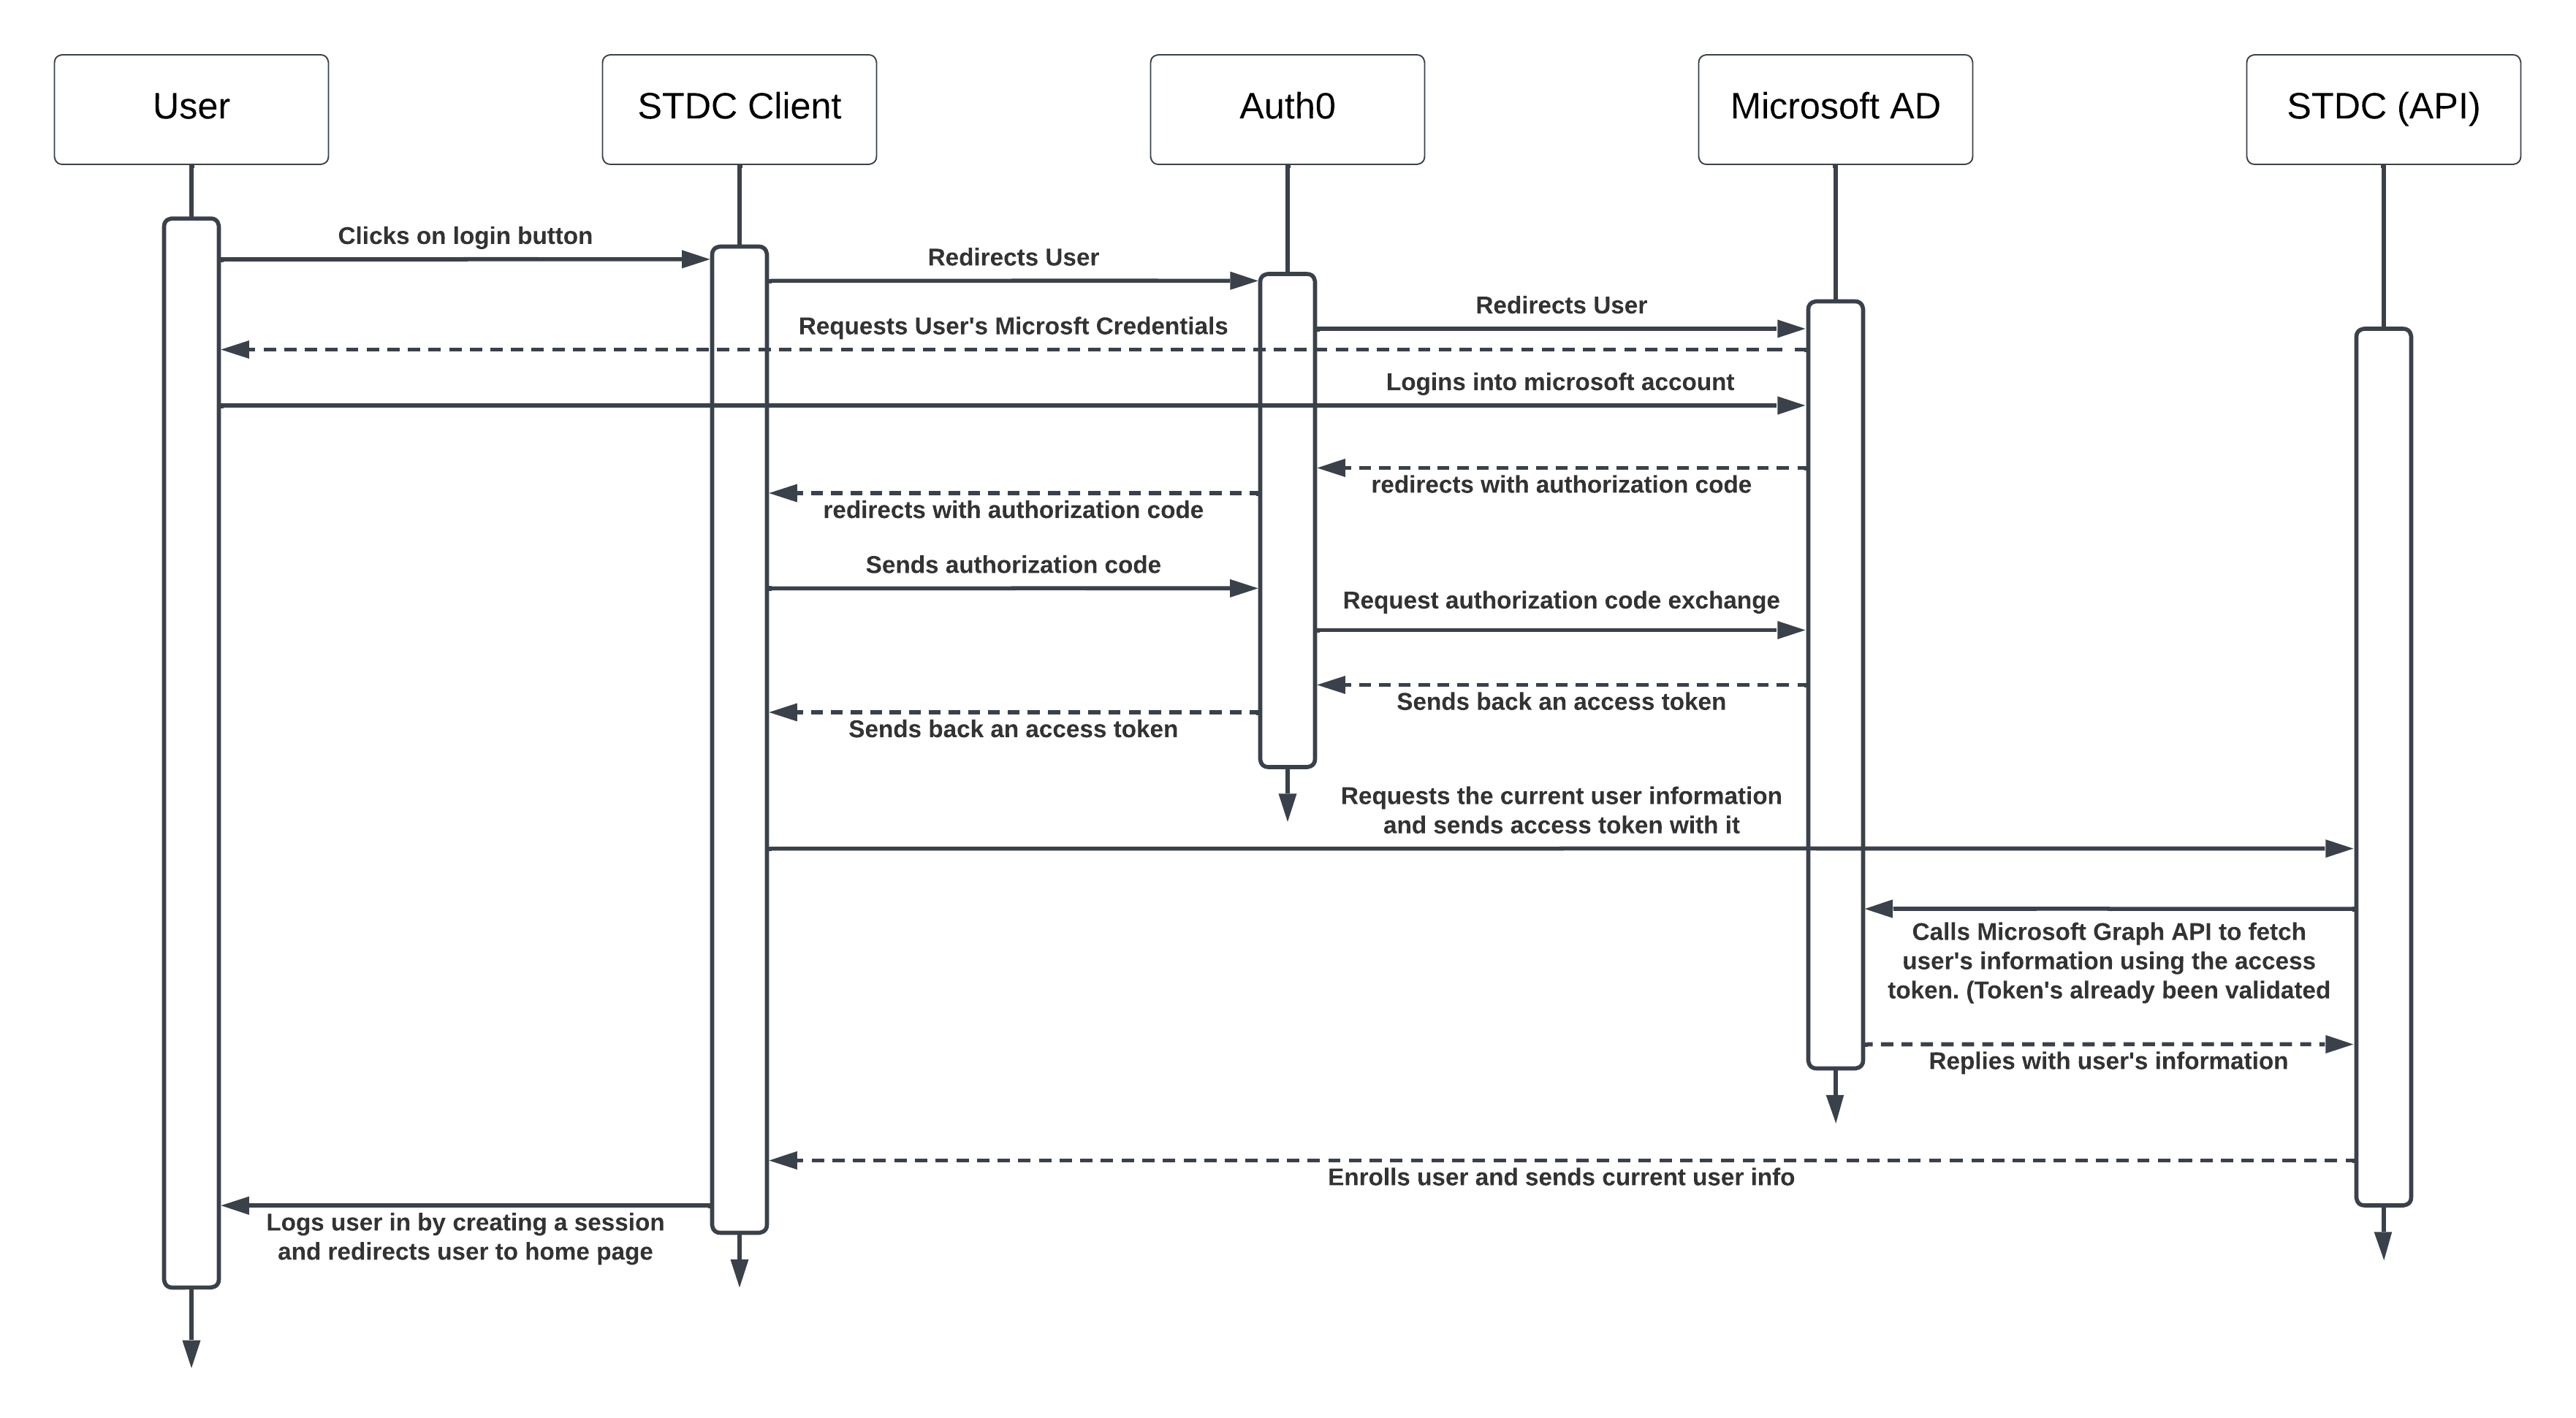
\includegraphics[width=150mm,scale=1]{figures/implementation_and_testing/implementation/backend/STDC Authentication.png}}
            \caption{OAuth2.0 Authorization Code Flow - STDC's Authentication Process}
        \end{figure}
    
    
        \vspace{-0.25cm}
        \newendline Please not that the OpenID Connect is an authentication layer on top of OAuth 2.0. It allows the user to login to the application using an identity provider (such as Microsoft, Google, Facebook, etc.). OpenID Connect is used in the STDC web application to get the user information from Microsoft.
    
        \vspace{0.25cm}
        \newendline Now that we have discussed how OAuth 2.0 and OpenID Connect works, let's discuss how the authentication process is handled in the STDC web application's backend because the above flow is an abstraction of how the general authentication happens in both client and server. The authentication process of the server side (backend) of STDC works as follows:
        
            
        \begin{itemize}
        \item The API is a Restful API, which means that it is stateless, and it does not store any information about the user. This means that the API does not know if the user is logged in or not, therefore each request is considered as a new request. This requires the client to send an access token with each request to the API.
        \item The client sends a request to the API with an access token. Now the API needs to verify the access token to make sure that it is valid and not expired. The STDC will allow the client access the resources only if the user is authenticated. Below here we will dive into some of the classes and modules responsible for the authentication process.\\
        
            \begin{itemize}
                \item AuthorizationService
                \item UsersService
                \item JsonWebToken
                \item GuardController
                \item CurrentUserConfigurable
                \item ApplicationController\\
            \end{itemize}
        \end{itemize}


        \vspace{0.25cm}
        \noindent\textbf{GuardController}
        
        \begin{figure}[H]
            \centerline{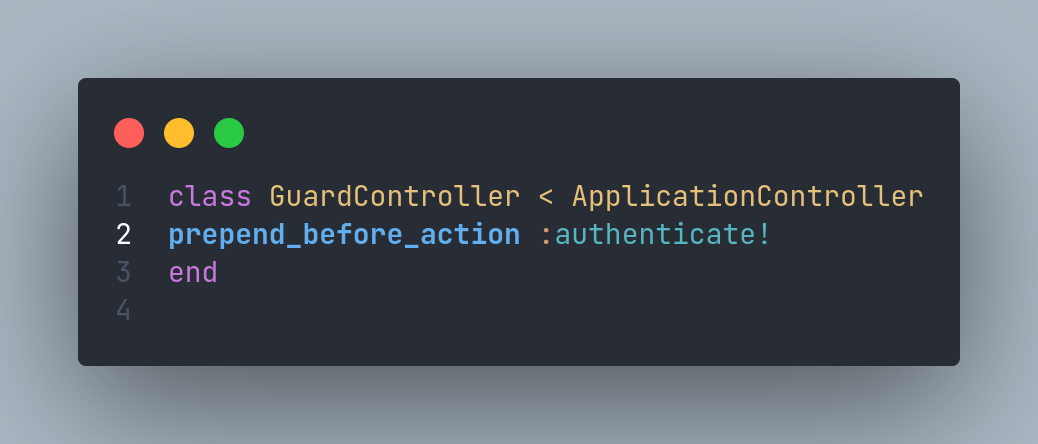
\includegraphics[width=150mm,scale=1]{figures/implementation_and_testing/implementation/backend/GuardController.png}}
            \caption{Authentication - GuardController}
        \end{figure}

        \newendline The GuardController is the base for every controller in the STDC application. The ApplicationController class which is a class defined by the Ruby on Rails framework is inherited by the GuardController. The GuardController calls a method called authenticate! before any action in any controller. The authenticate! method is defined the CurrentUserConfigurable module which is included in the ApplicationController.\\


        \clearpage
        \noindent\textbf{CurrentUserConfigurable}
        
        \begin{figure}[H]
            \centerline{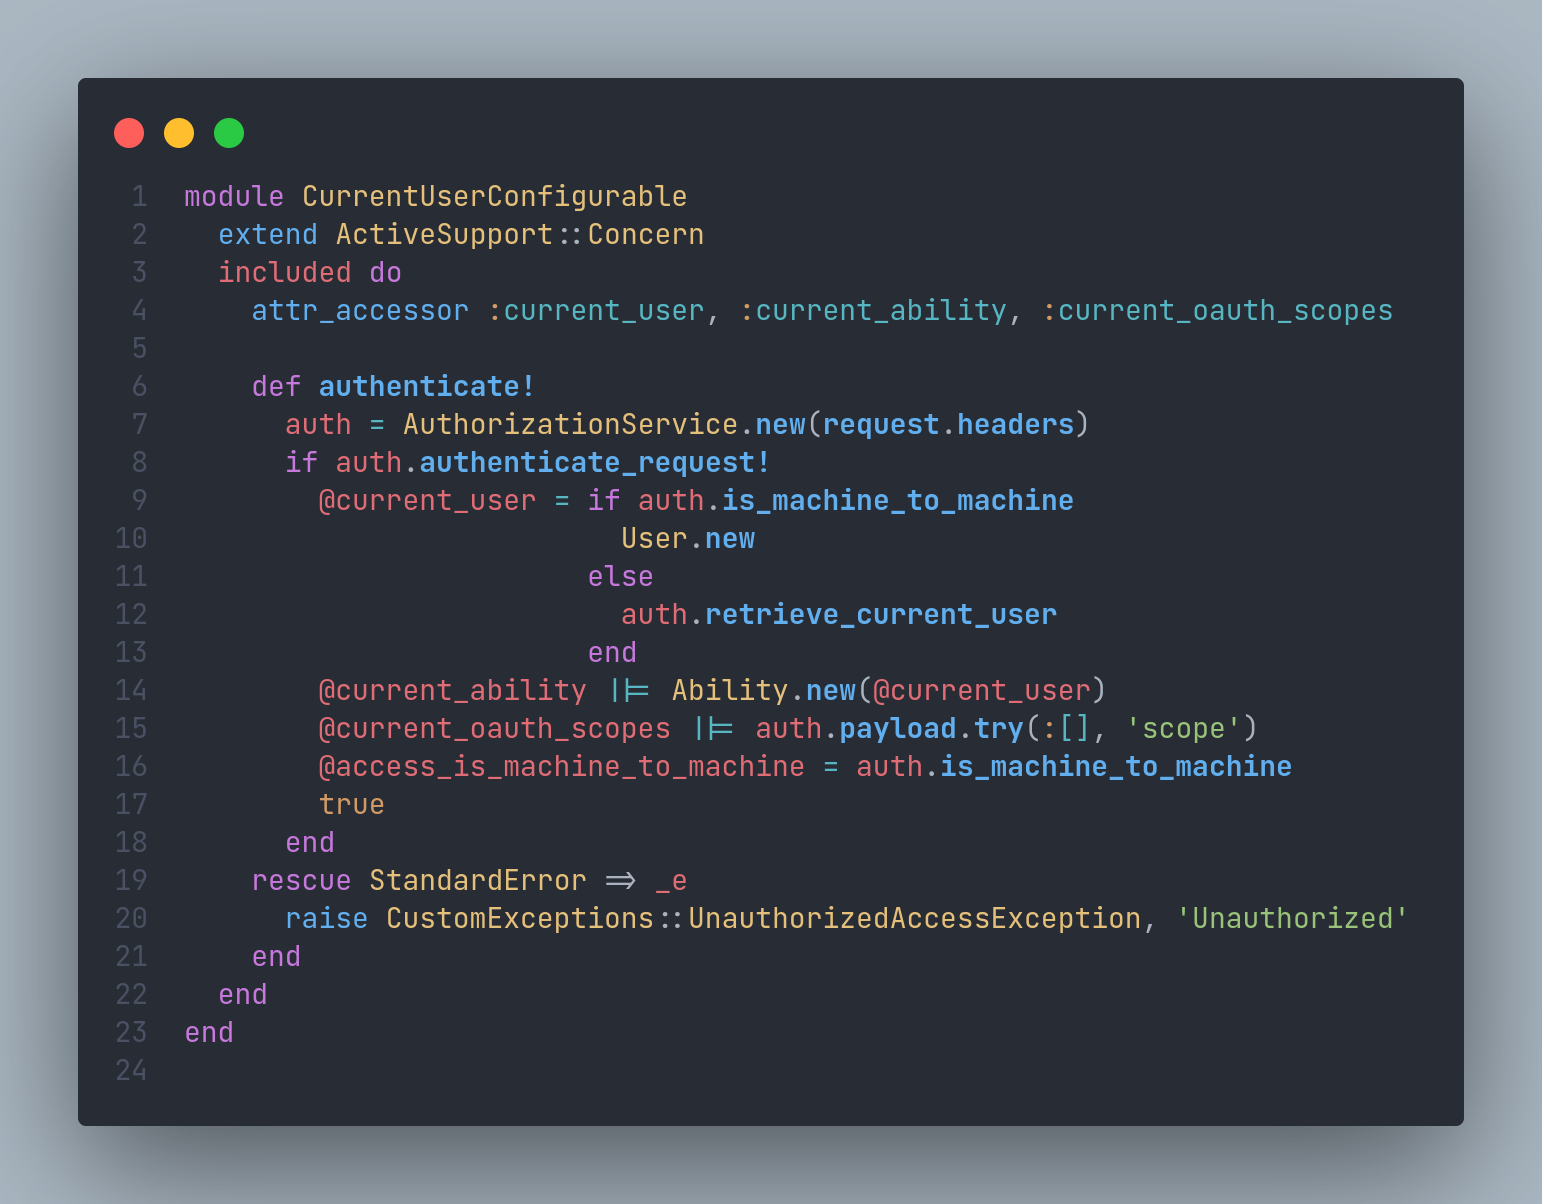
\includegraphics[width=150mm,scale=1]{figures/implementation_and_testing/implementation/backend/CurrentUserConfigurable.png}}
            \caption{Authentication - CurrentUserConfigurable}
        \end{figure}

        \newendline The CurrentUserConfigurable is a module that is included in the ApplicationController. The authenticate! method is responsible for authenticating the user. It works as follows:

            \begin{itemize}
                \item The authenticate! method calls the authenticate\_request! method in the AuthorizationService class.
                \item If the authenticate\_request! method returns true, then the authenticate! method will set the current\_user, current\_ability, and current\_oauth\_scopes instance variables.
                \item If the authenticate\_request! method returns false, then the authenticate! method will raise an exception.\\
            \end{itemize}


        \vspace{0.25cm}
        \noindent\textbf{AuthorizationService}
        
        \begin{figure}[H]
            \centerline{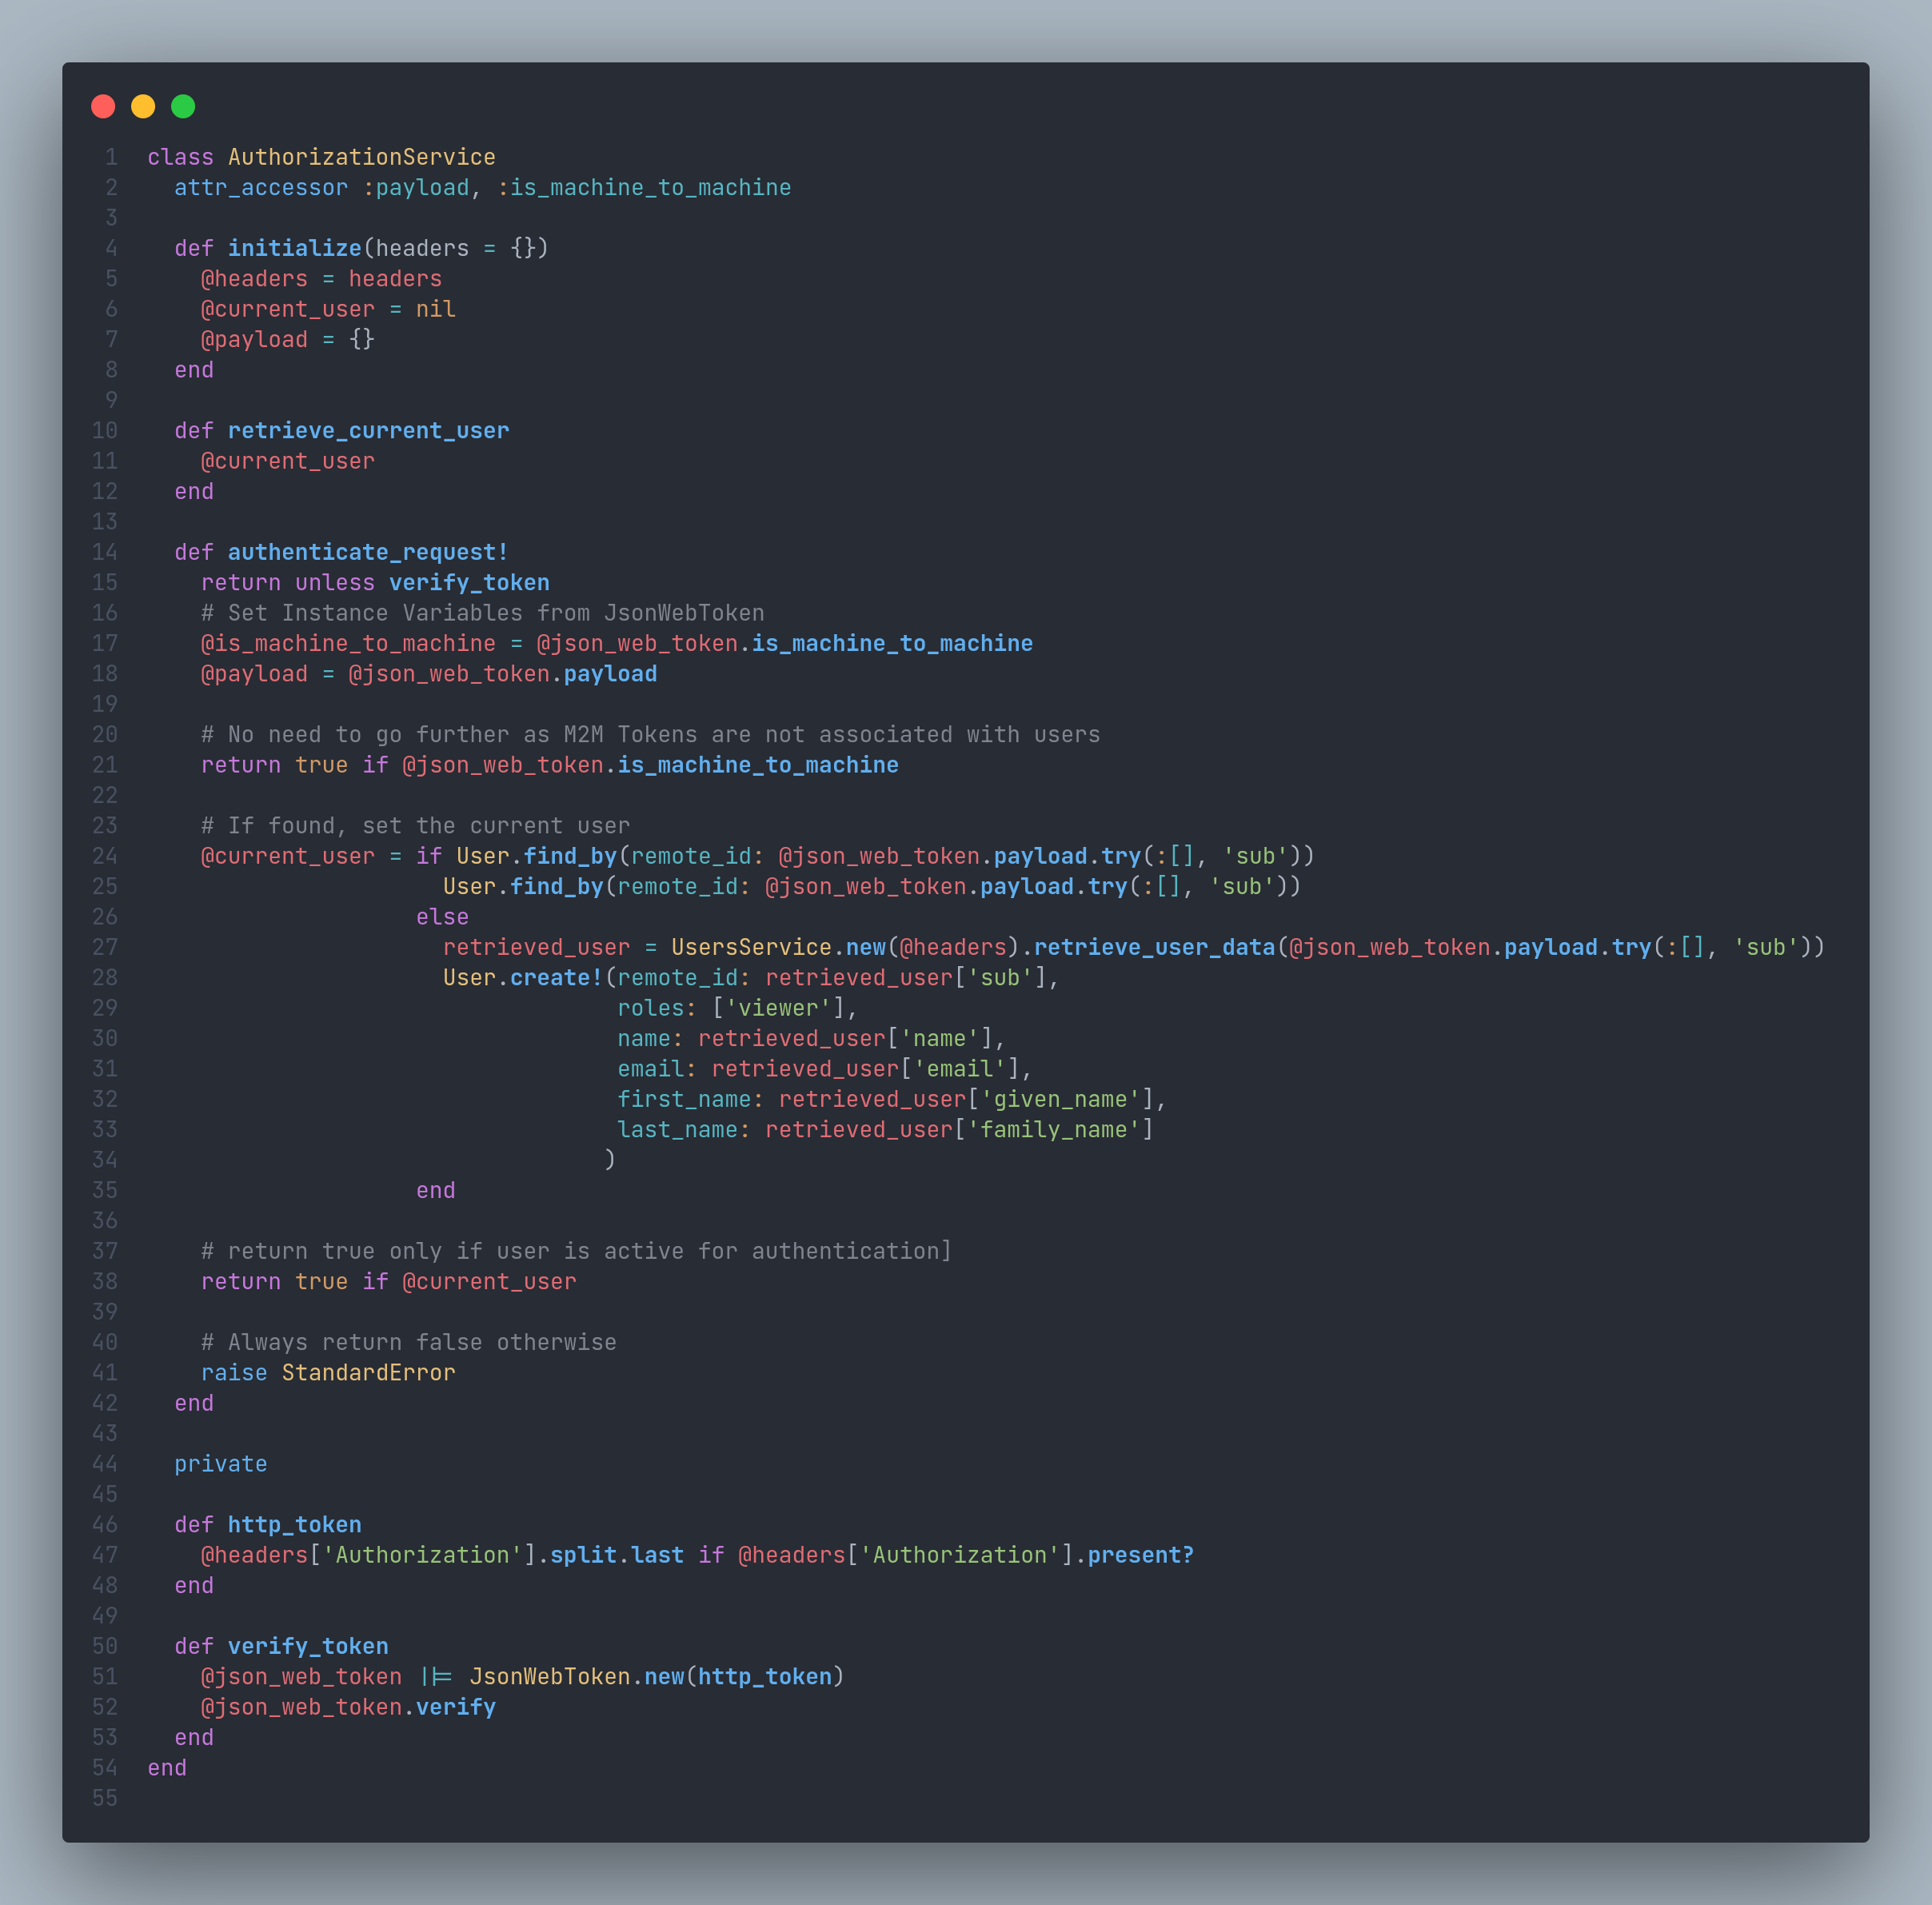
\includegraphics[width=150mm,scale=1]{figures/implementation_and_testing/implementation/backend/AuthorizationService.png}}
            \caption{Authentication - AuthorizationService}
        \end{figure}

        \newendline The AuthorizationService class is responsible for authenticating the user. It works as follows:

            \begin{itemize}
                \item The AuthorizationService class has a method called authenticate\_request! which is called by the authenticate! method in the CurrentUserConfigurable module.
                \item The authenticate\_request! first calls the verify\_token method to verify the access token.
                \item If the verify\_token method returns true, then the authenticate\_request! method will set the payload and is\_machine\_to\_machine instance variables.
                \item If the verify\_token method returns false, then the authenticate\_request! method will raise an exception.
                \item If the is\_machine\_to\_machine instance variable is true, then the authenticate\_r- equest! method will return true.
                \item If the is\_machine\_to\_machine instance variable is false, then the authenticate\_request! method will call the retrieve\_current\_user method to retrieve the current user information.
                \item Once the current user information is retrieved, the authenticate\_request! method will return true.
                \item If the retrieve\_current\_user method returns nil, then the authenticate\_request! method will raise an exception.\\
            \end{itemize}

        \clearpage
        \noindent\textbf{JsonWebToken}
        
        \begin{figure}[H]
            \centerline{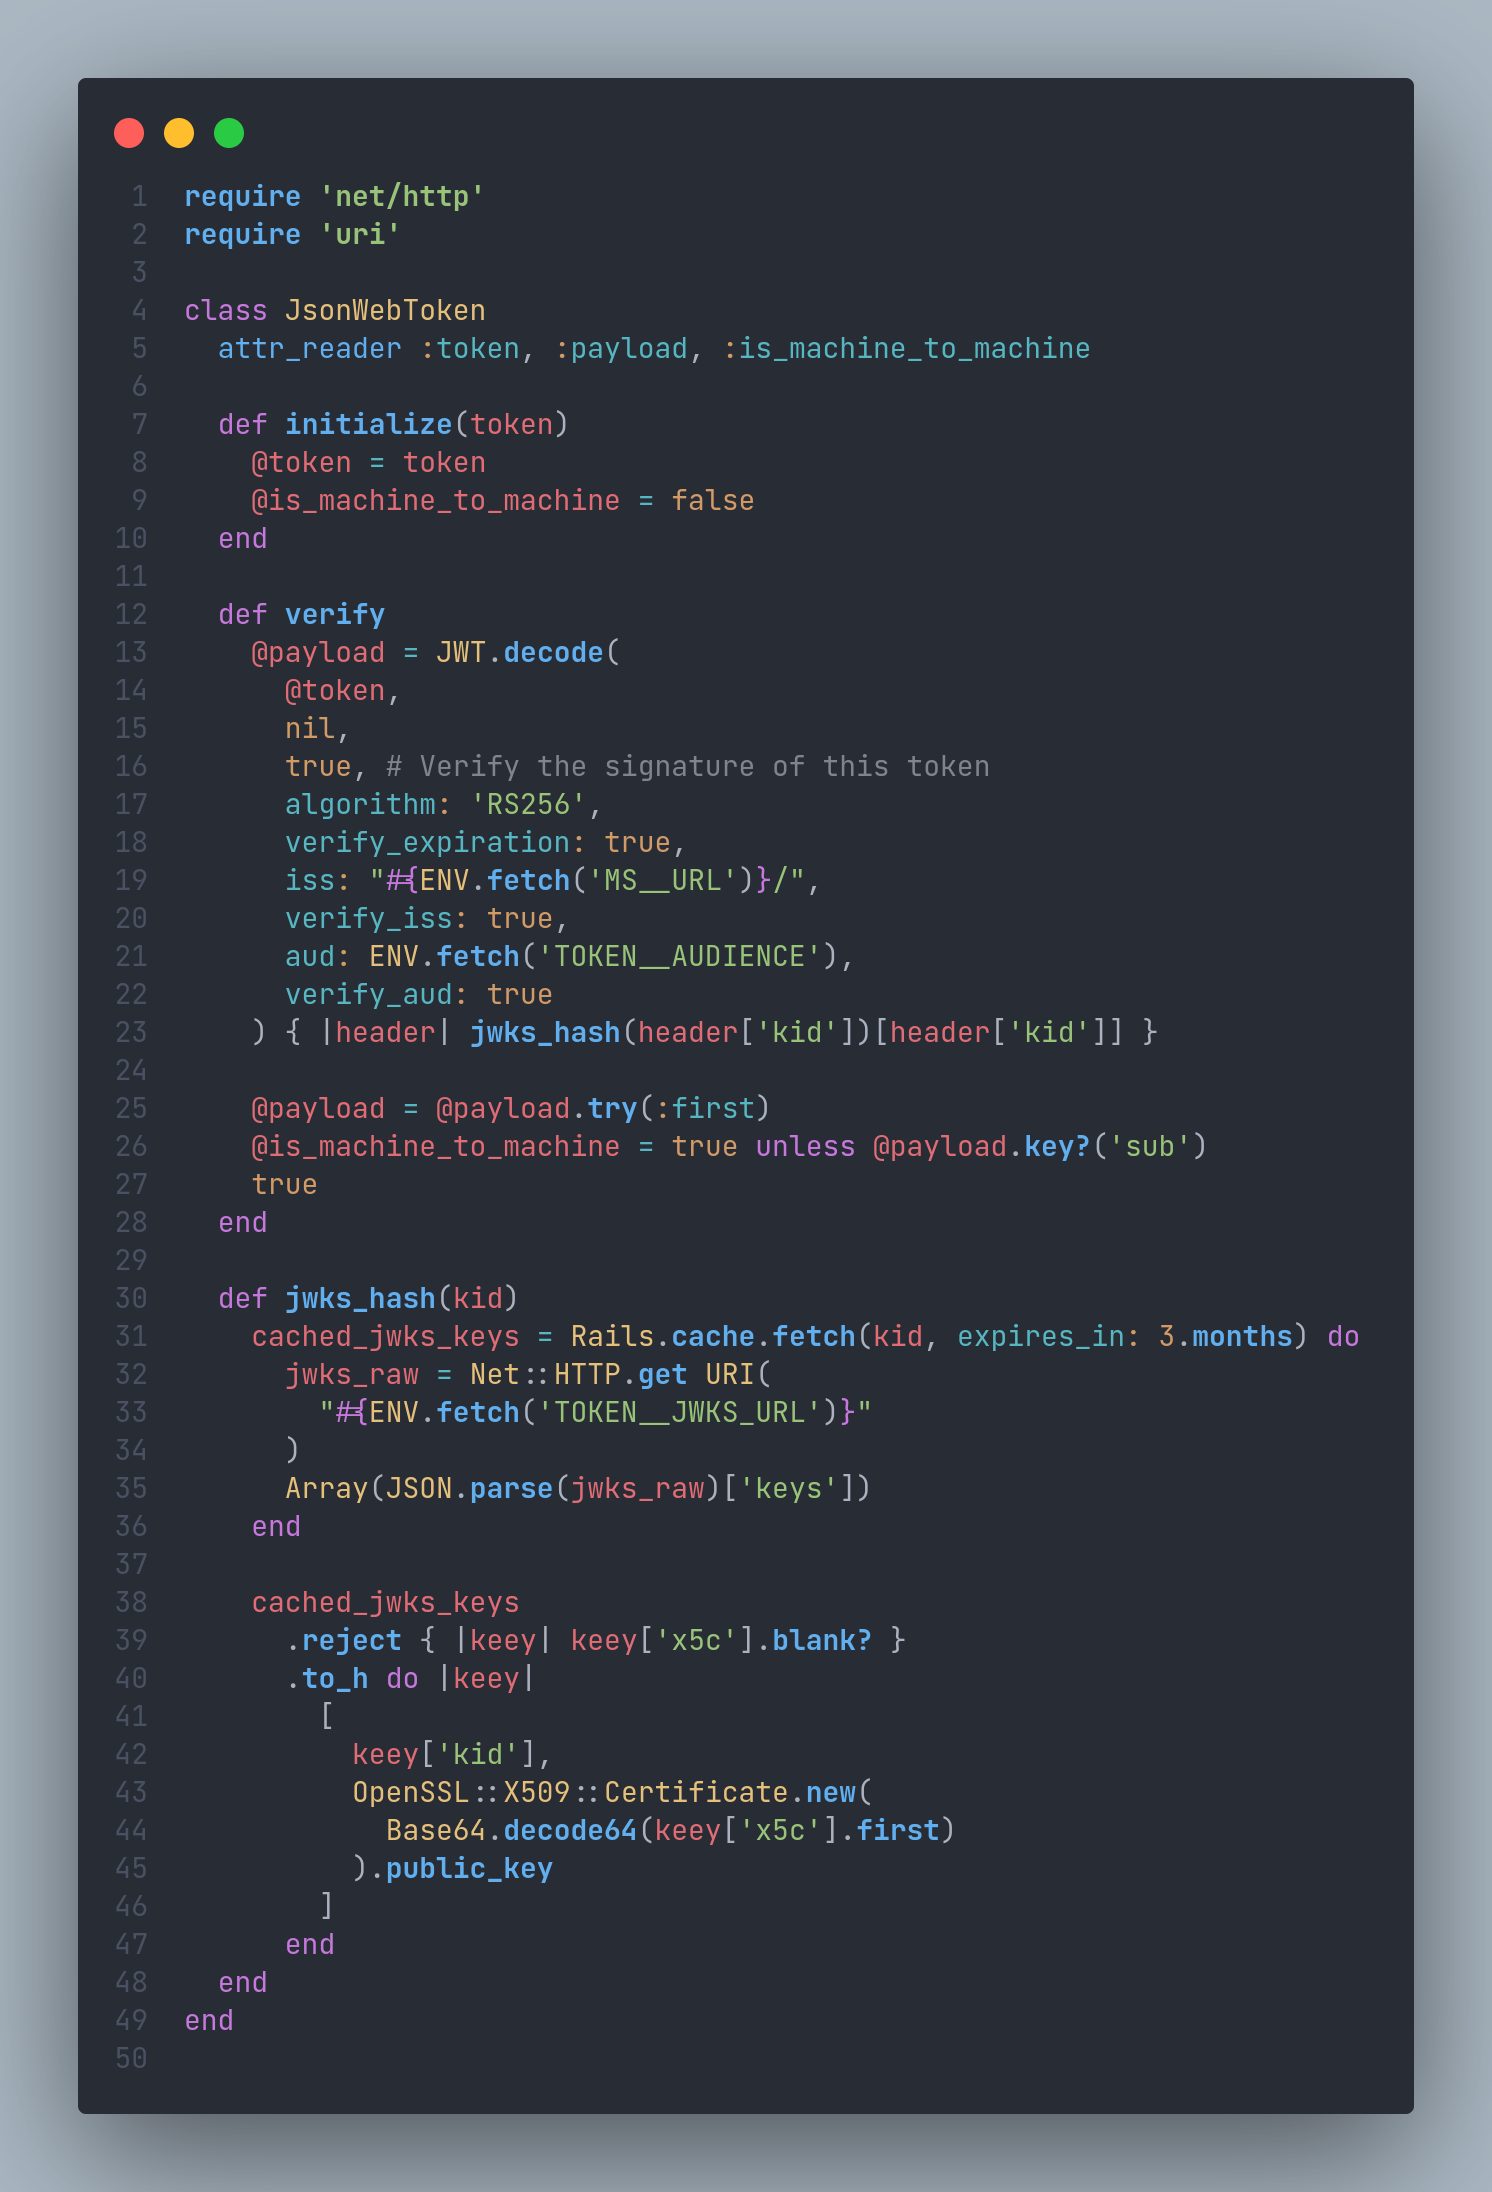
\includegraphics[width=150mm,scale=1]{figures/implementation_and_testing/implementation/backend/JsonWebToken.png}}
            \caption{Authentication - JsonWebToken}
        \end{figure}

        \newendline The JsonWebToken class is responsible for verifying the access token. It works as follows:

            \begin{itemize}
                \item The JsonWebToken class has a method called verify which is called by the verify\_token method in the AuthorizationService class.
                \item The verify method first calls the jwks\_hash method to get the public key of the Auth0 application that has been setup prior to the development of the STDC web application.
                \item The verify method then calls the JWT.decode method to decode the access token.

                \vspace{0.25cm}
                \newendline While decoding the access token, the JWT.decode method will verify the access token using the public key that has been retrieved from the jwks\_hash method. If the access token is valid, then the JWT.decode method will return true, otherwise it will return false. For validation, the JWT.decode method will check the following:
                    \begin{itemize}
                        \item The signature of the access token.
                        \item The expiration of the access token.
                        \item The issuer of the access token.
                        \item The audience of the access token.
                    \end{itemize}

                \item If the JWT.decode method returns true, then the verify method will set the payload and is\_machine\_to\_machine instance variables.
                \item If the JWT.decode method returns false, then the verify method will raise an exception.\\
            \end{itemize}

        \clearpage
        \noindent \textbf{UsersService}
        
        \begin{figure}[H]
            \centerline{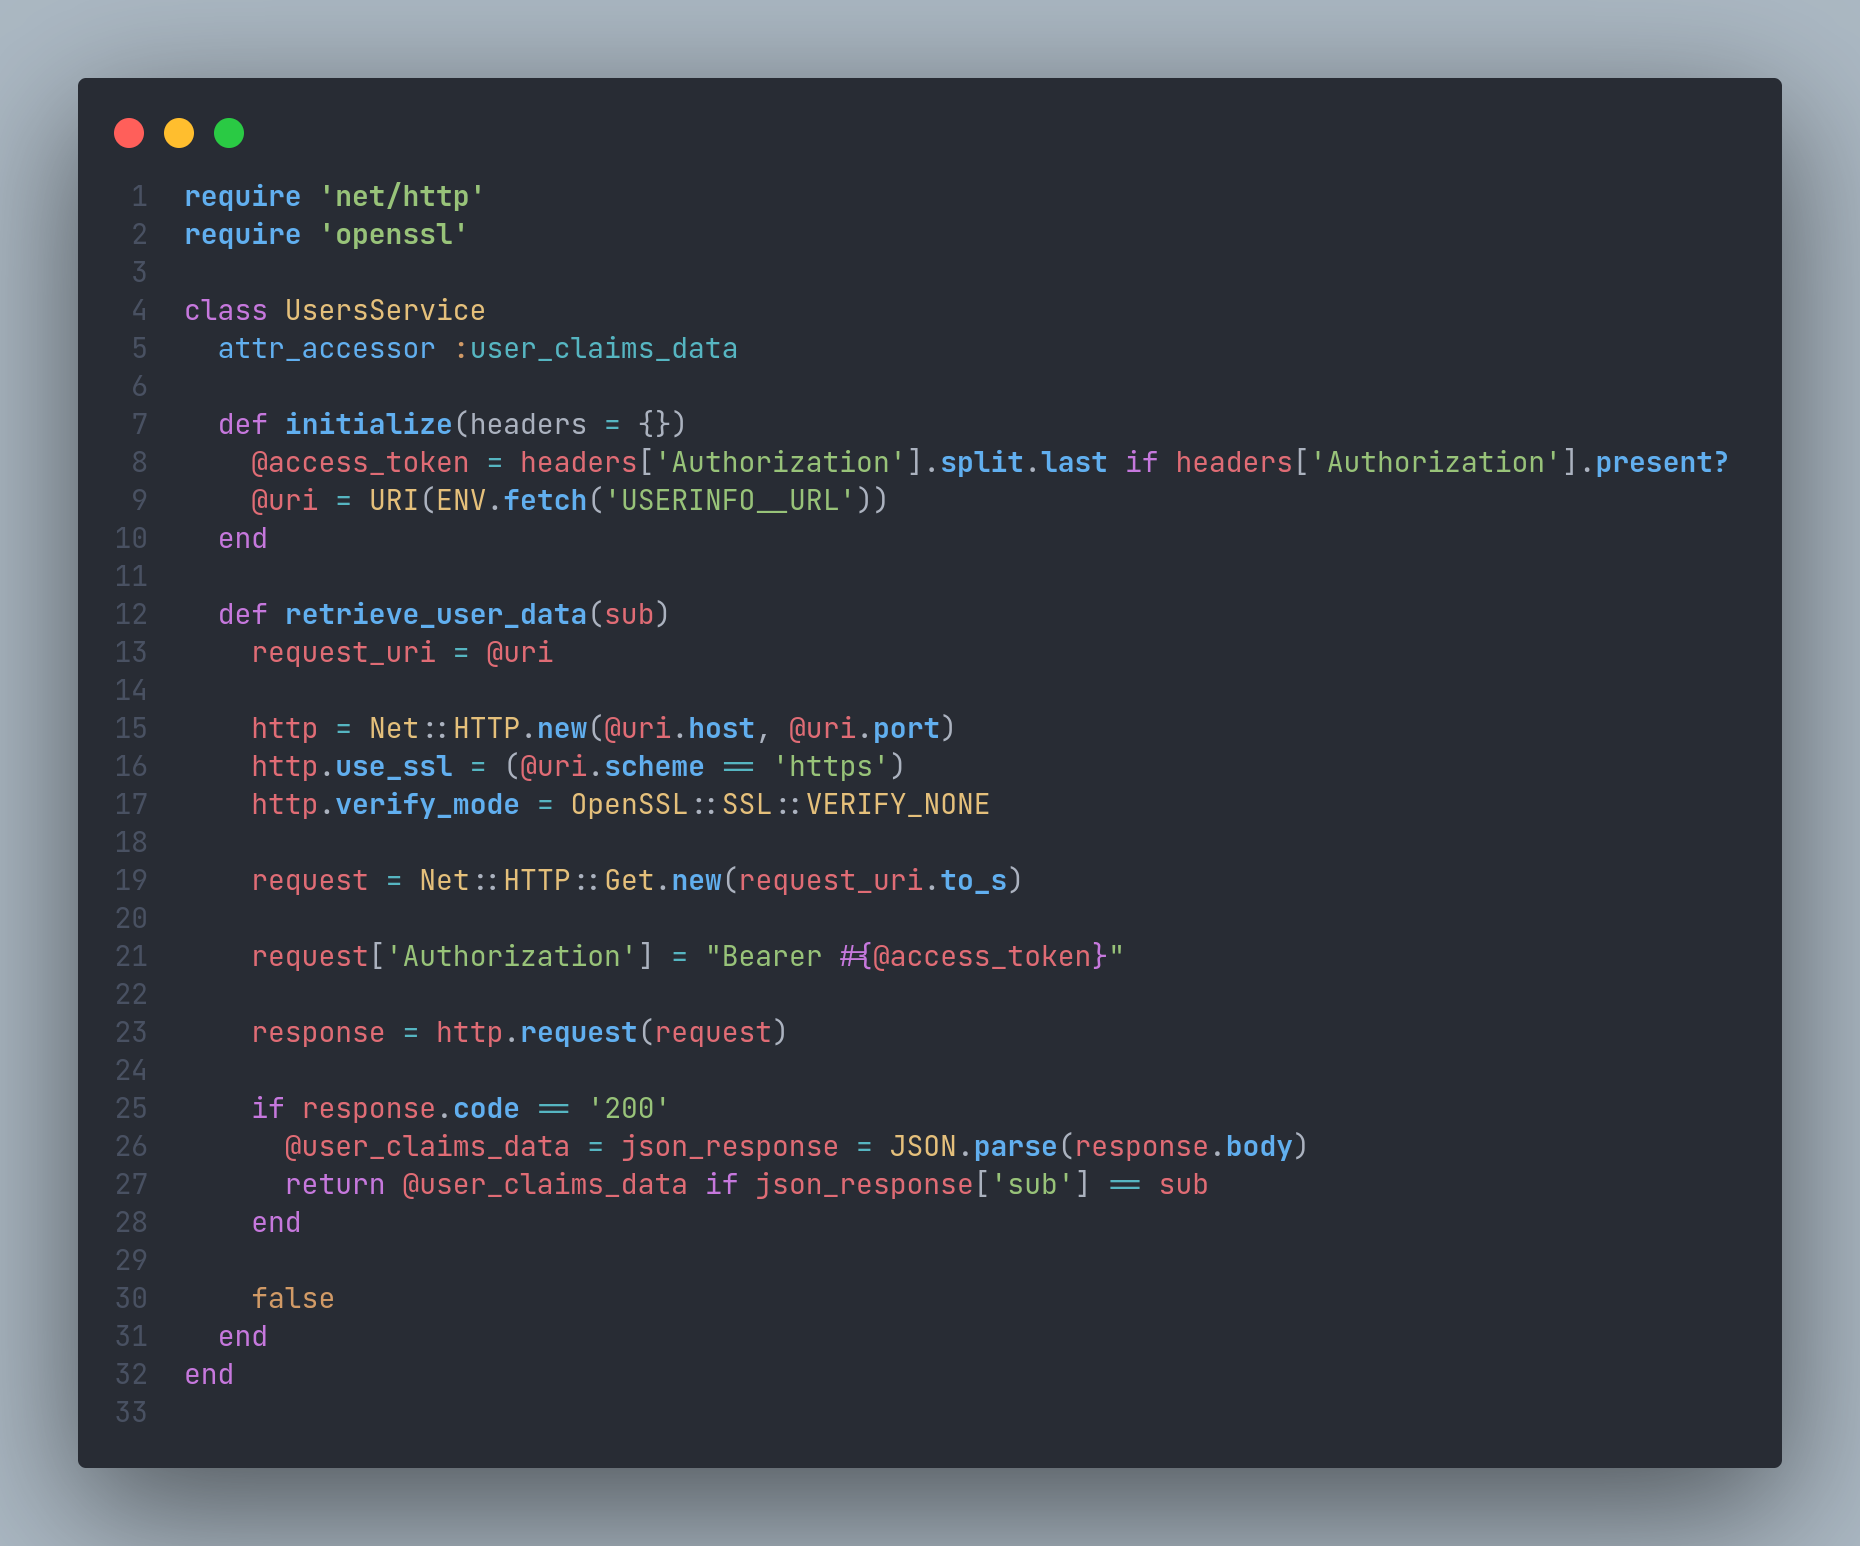
\includegraphics[width=150mm,scale=1]{figures/implementation_and_testing/implementation/backend/UsersService.png}}
            \caption{Authentication - UsersService}
        \end{figure}
        
        \newendline The UsersService class is responsible for retrieving the user information from Microsoft. It works as follows:

            \begin{itemize}
                \item The UsersService class has a method called retrieve\_user\_data which is called by the retrieve\_current\_user method in the AuthorizationService class.
                \item The retrieve\_user\_data first tries to fetch the API access token from the headers of the request.
                \item The retrieve\_user\_data then sends a request to Microsoft to get the user information to Microsoft's userinfo endpoint.
                \item If the request is successful, then the retrieve\_user\_data method will set the user information to current\_user and then return true, else it will return false.
            \end{itemize}

        \vspace{0.25cm}
        \newendline Now that all the classes and modules have been explained, we understand a few advantageous of the explained authentication process:

            \begin{itemize}
                \item The authentication process is handled in the backend, which means that the client does not have to worry about the authentication process. Even if the client is compromised, the attacker will not be able to access the API without a valid access token.
                \item The usage of the OAuth 2.0 and OpenID Connect allows the STDC web application to be more secure, since the authentication process is handled by Auth0 and Microsoft.
                \item The API does not store user's credentials, which means that if the API were to be compromised, the attacker will not be able to access the user's credentials.
                \item The authentication process allows for multiple checks to be done to make sure that the access token is valid. If the access token has been tempered with, then the authentication process will fail since the signature of the access token will not match the signature of the public key obtained from the jwks of Auth0.
                \item Using a JWT access token gives the API the ability to verify the access token without having to make a request to Auth0 or Microsoft.
            \end{itemize}
    
    \clearpage

    % ==============================================================
    % ==============================================================
    % ==============================================================



    \vspace{0.25cm}
    \newendline \textbf{\textit{Authorization}}\newendline
        The Student Talent Development Center (STDC) makes use of Cancancan to handle its authorization. Cancancan is an authorization library for Ruby on Rails which restricts what resources a given user is allowed to access. All permissions are defined in a single location (the Ability class) and not duplicated across controllers, views, and database queries. The following are the benefits of using Cancancan:

        \begin{itemize}
            \item Cancancan allows for the definition of permissions in a very simple and readable way.
            \item Cancancan allows for the definition of permissions in a very small and granular way.
            \item Cancancan allows for running queries on the database based on the permissions.
        \end{itemize}

        \vspace{0.25cm}
        \newendline In the coming pages, we will discuss how Cancancan is used in the STDC web application.

        \vspace{0.25cm}
        \newendline In the STDC web application, the permissions are defined in the Ability class. The Ability class is a class defined by Cancancan, and it is responsible for defining the permissions. The Ability class is defined as follows:


        %%%%%%%%%%%%%%%%%%%%%%%%%%%%%%%%%%%%%%%%%%%%%%%%%%%%%%%%%%%%%%%%%%
        %%%%%%%%%%%%%%%%%%%%%%%%%%%%%%%%%%%%%%%%%%%%%%%%%%%%%%%%%%%%%%%%%%
        %%%%%%%%%%%%%%%%%%%%%%%%%%%%%%%%%%%%%%%%%%%%%%%%%%%%%%%%%%%%%%%%%%
        

        \begin{figure}[H]
            \centerline{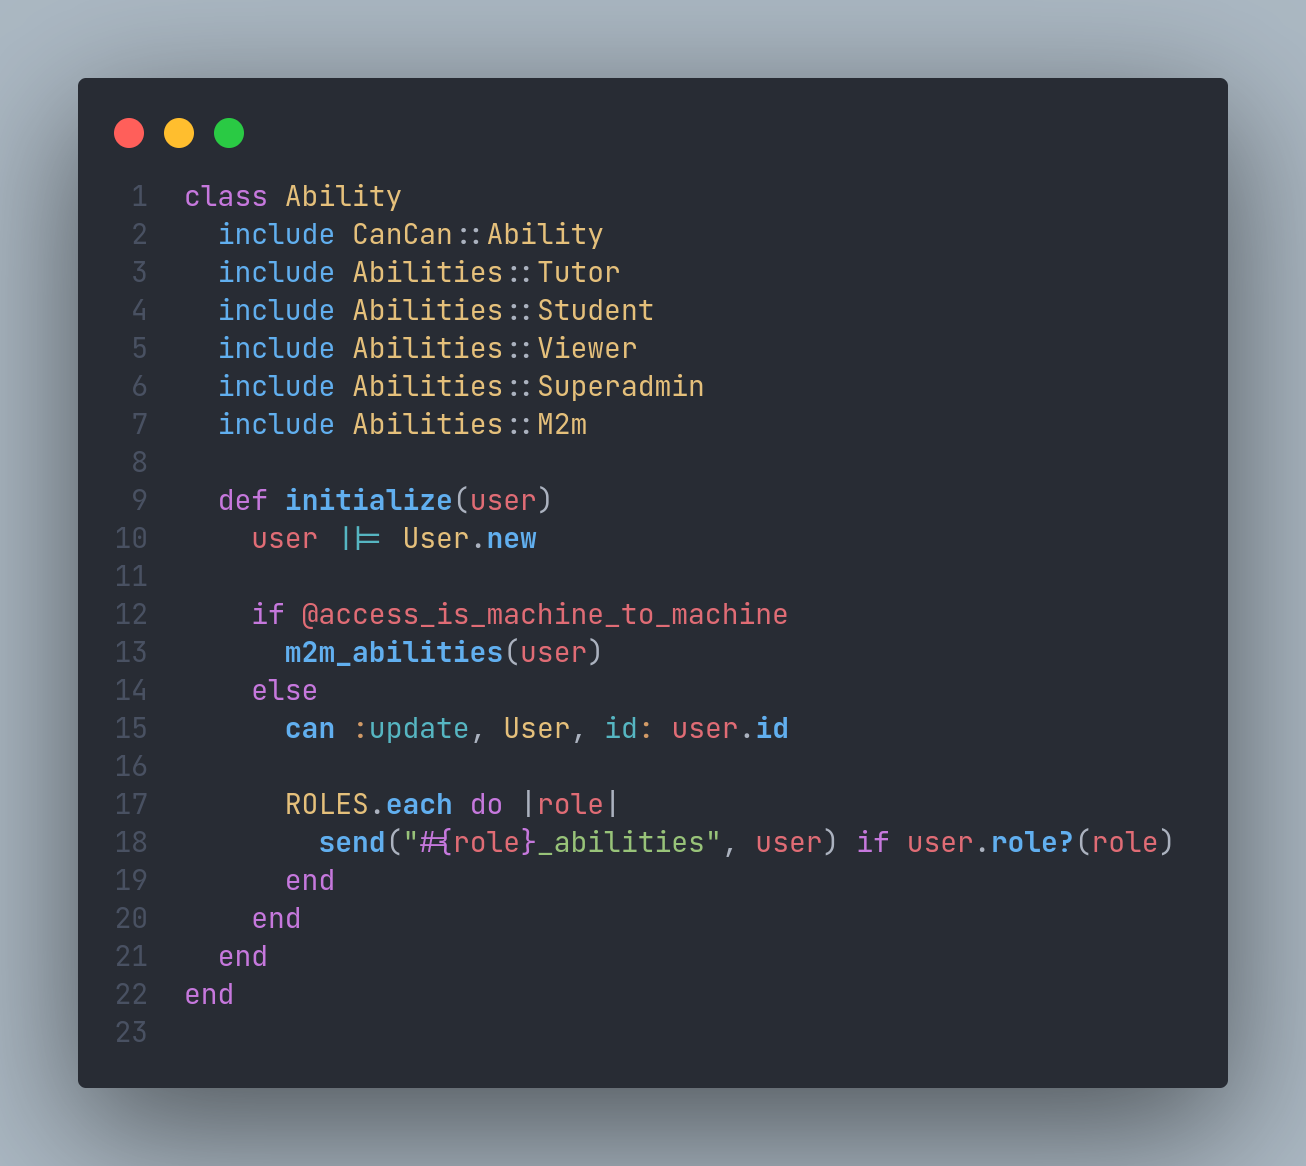
\includegraphics[width=150mm,scale=1]{figures/implementation_and_testing/implementation/backend/Ability.png}}
            \caption{Authorization - Ability}
        \end{figure}

        \newendline The Ability class works as follows:

            \begin{itemize}
                \item The Ability class has a method called initialize which is called by the Ability class itself.
                \item The initialize method first checks if the user is a machine to machine user or not.
                \item If the user is a machine to machine user, then the initialize method will call the m2m\_abilities method to define the permissions for the machine to machine user.
                \item If the user is not a machine to machine user, then the initialize method will call the role\_abilities method to define the permissions for the user based on his/her role.
                \item The initialize method will then return the permissions.
            \end{itemize}


        \vspace{0.25cm}
        \newendline The CanCanCan gem has a method called can which is defined by Cancancan. The can method is used to define the permissions for a user. The can method takes three parameters, the first parameter is the action, the second parameter is the resource, and the third parameter is the conditions. The action parameter is the action that the user is allowed to perform on the resource. The resource parameter is the resource that the user is allowed to perform the action on. The conditions parameter is the conditions that the user is allowed to perform the action on the resource.

        \vspace{0.25cm}
        \newendline The Ability class has a method called m2m\_abilities which is responsible for defining the permissions for the machine to machine user. The m2m\_abilities method is defined as follows:

        \begin{figure}[H]
            \centerline{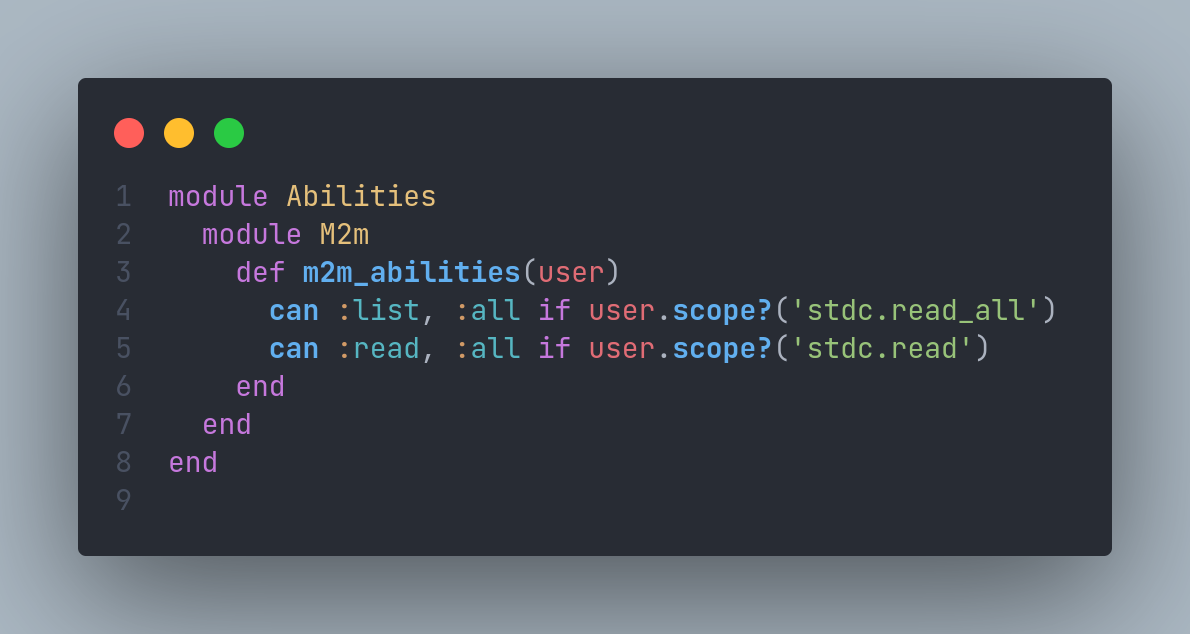
\includegraphics[width=150mm,scale=1]{figures/implementation_and_testing/implementation/backend/M2mAbilities.png}}
            \caption{Authorization - m2m\_abilities}
        \end{figure}

        \newendline The m2m\_abilities method defines the permissions for the machine to machine user as follows:
                    \begin{itemize}
                        \item The machine to machine user can read any resource.
                        \item The machine to machine user can list any resource.
                    \end{itemize}

        \vspace{0.25cm}
        \newendline The Ability class has a method called superadmin\_abilities which is responsible for defining the permissions for the superadmin user. The superadmin\_abilities method is defined as follows:

            \begin{figure}[H]
                \centerline{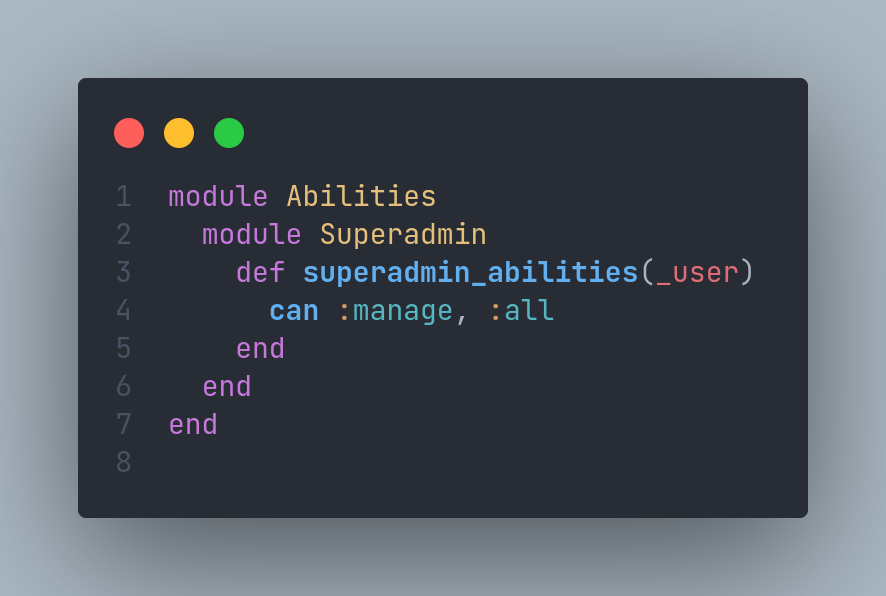
\includegraphics[width=150mm,scale=1]{figures/implementation_and_testing/implementation/backend/SuperadminAbilities.png}}
                \caption{Authorization - superadmin\_abilities}
            \end{figure}

            \vspace{0.25cm}
            \newendline The superadmin\_abilities method defines the permissions for the superadmin user as follows:
                \begin{itemize}
                    \item The superadmin can manage any resource.
                \end{itemize}


        \vspace{0.25cm}
        \newendline The Ability class has a method called tutor\_abilities which is responsible for defining the permissions for the tutor user. The tutor\_abilities method is defined as follows:
            
            \begin{figure}[H]
                \centerline{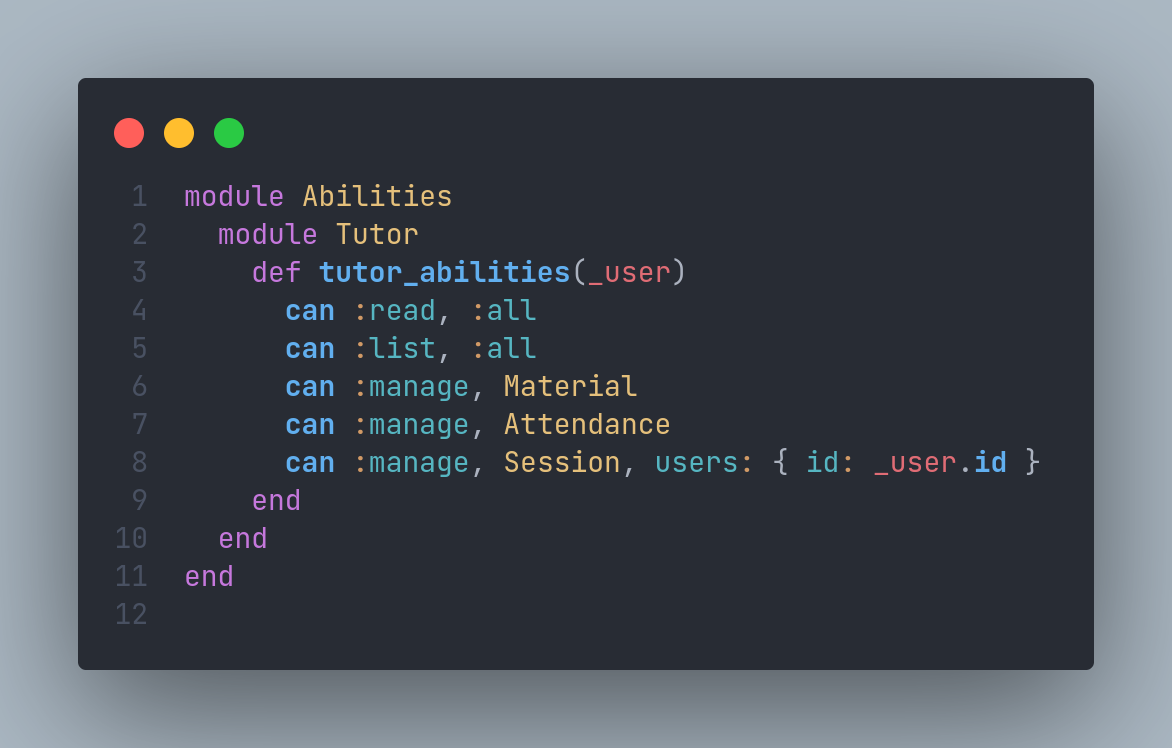
\includegraphics[width=150mm,scale=1]{figures/implementation_and_testing/implementation/backend/TutorAbilities.png}}
                \caption{Authorization - tutor\_abilities}
            \end{figure}

            \vspace{0.25cm}
            \newendline The tutor\_abilities method defines the permissions for the tutor user as follows:
            
            \begin{itemize}
                \item The tutor can read any resource.
                \item The tutor can list any resource.
                \item The tutor can manage the material resource.
                \item The tutor can manage the attendance resource.
                \item The tutor can manage the session resource if he/she is the owner of the session.
            \end{itemize}

        \vspace{0.25cm}
        \newendline The Ability class has a method called student\_abilities which is responsible for defining the permissions for the student user. The student\_abilities method is defined as follows:
            
            \begin{figure}[H]
                \centerline{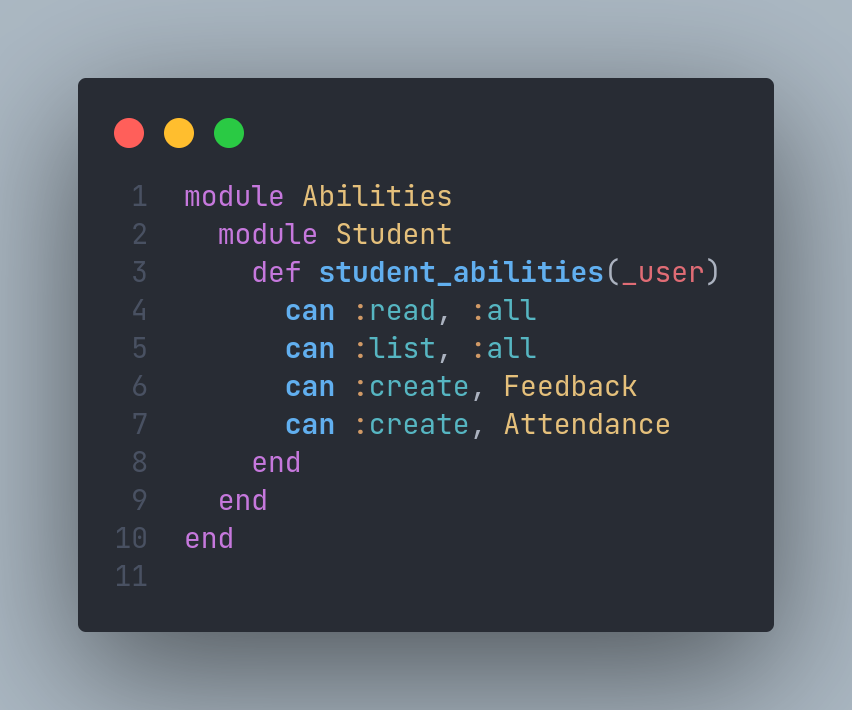
\includegraphics[width=150mm,scale=1]{figures/implementation_and_testing/implementation/backend/StudentAbilities.png}}
                \caption{Authorization - student\_abilities}
            \end{figure}

            \vspace{0.25cm}
            \newendline The student\_abilities method defines the permissions for the student user as follows:
            \begin{itemize}
                \item The student can read any resource.
                \item The student can list any resource.
                \item The student can create the feedback resource.
                \item The student can create the attendance resource.\\
            \end{itemize}

    \vspace{0.25cm}
    \newendline The STDC web application's security when it comes to authorization has a few advantages, one of which is small granular permissions. The STDC web application's permissions are defined in a very small and granular way, which means that the permissions are defined for each action on each resource. This allows for more control over the permissions, and it allows for more flexibility when it comes to defining the permissions. In case a user is compromised and his/her access token is stolen, the attacker will not be able to access the resources that the user is not authorized to access. This is because the permissions are defined in a very small and granular way, allows for minimal damage in case of a security breach.
    
    \clearpage

    %%%%%%%%%%%%%%%%%%%%%%%%%%%%%%%%%%%%%%%%%%%%%%%%%%%%%%%%%%%%%%%%%%
    %%%%%%%%%%%%%%%%%%%%%%%%%%%%%%%%%%%%%%%%%%%%%%%%%%%%%%%%%%%%%%%%%%
    %%%%%%%%%%%%%%%%%%%%%%%%%%%%%%%%%%%%%%%%%%%%%%%%%%%%%%%%%%%%%%%%%%

    \vspace{0.25cm}
    \newendline \textbf{\textit{Models}}\newendline
        A model in the context of the Student Talent Development Center (STDC)  web application typically encompasses various components that define its behavior and structure. These components include concerns, enums, validations, callbacks, associations, scopes, and methods. Each of these elements plays a crucial role in defining the characteristics and functionality of the model.
        
        \vspace{0.25cm}
        \newendline The Student Talent Development Center (STDC) application consists of multiple models, including answer, attendance, course, enrollment, feedback, material, question, session, and user. Each model shares a similar structure with the course (which will be explained in detail below) model and exhibits similar behaviors and functionalities.
        
        \vspace{0.25cm}
        \newendline Validations are used to ensure the integrity and validity of the data stored in a model. They define rules and constraints that must be met for the model to be considered valid. For example, the presence validation ensures that a specific attribute, such as the name of a course, is not empty. If the validation fails, the object will not be saved.
        
        \vspace{0.25cm}
        \newendline Enums are used to define a set of discrete values for an attribute. They allow for a more expressive and structured representation of certain attributes. In the context of the STDC application, enums are used to define values such as the status of a course (e.g., active or inactive). The actual values stored in the database are typically integers corresponding to the enum values, and Rails provides helper methods to convert between the integer and enum values.

        \begin{figure}[H]
            \centerline{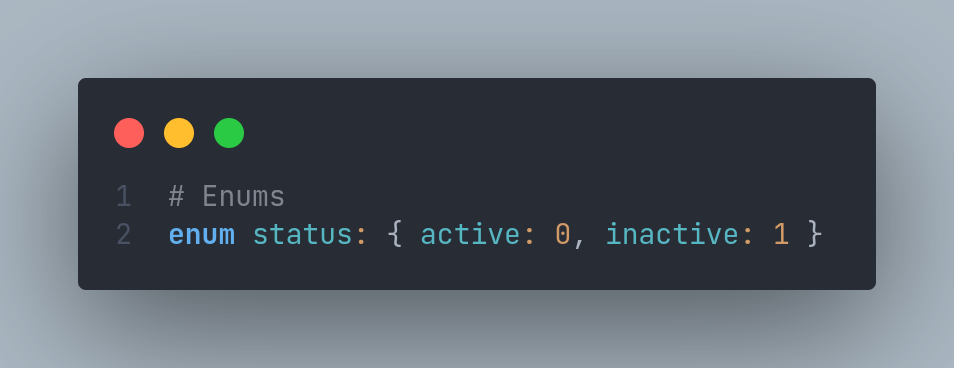
\includegraphics[width=115mm,scale=1]{figures/implementation_and_testing/implementation/backend/course_enums.png}}
            \caption{Course Model - Enums}
        \end{figure}

        
        \vspace{0.25cm}
        \newendline Methods in a model encapsulate business logic and define additional behaviors. They are used to perform calculations, retrieve related data, or implement custom functionality. For example, in the course model, there are methods like "tutor\_name" to retrieve the name of the tutor for the course, "next\_session\_date" to determine the date of the next session, and "rating" to retrieve the rating of the course.

        \begin{figure}[H]
            \centerline{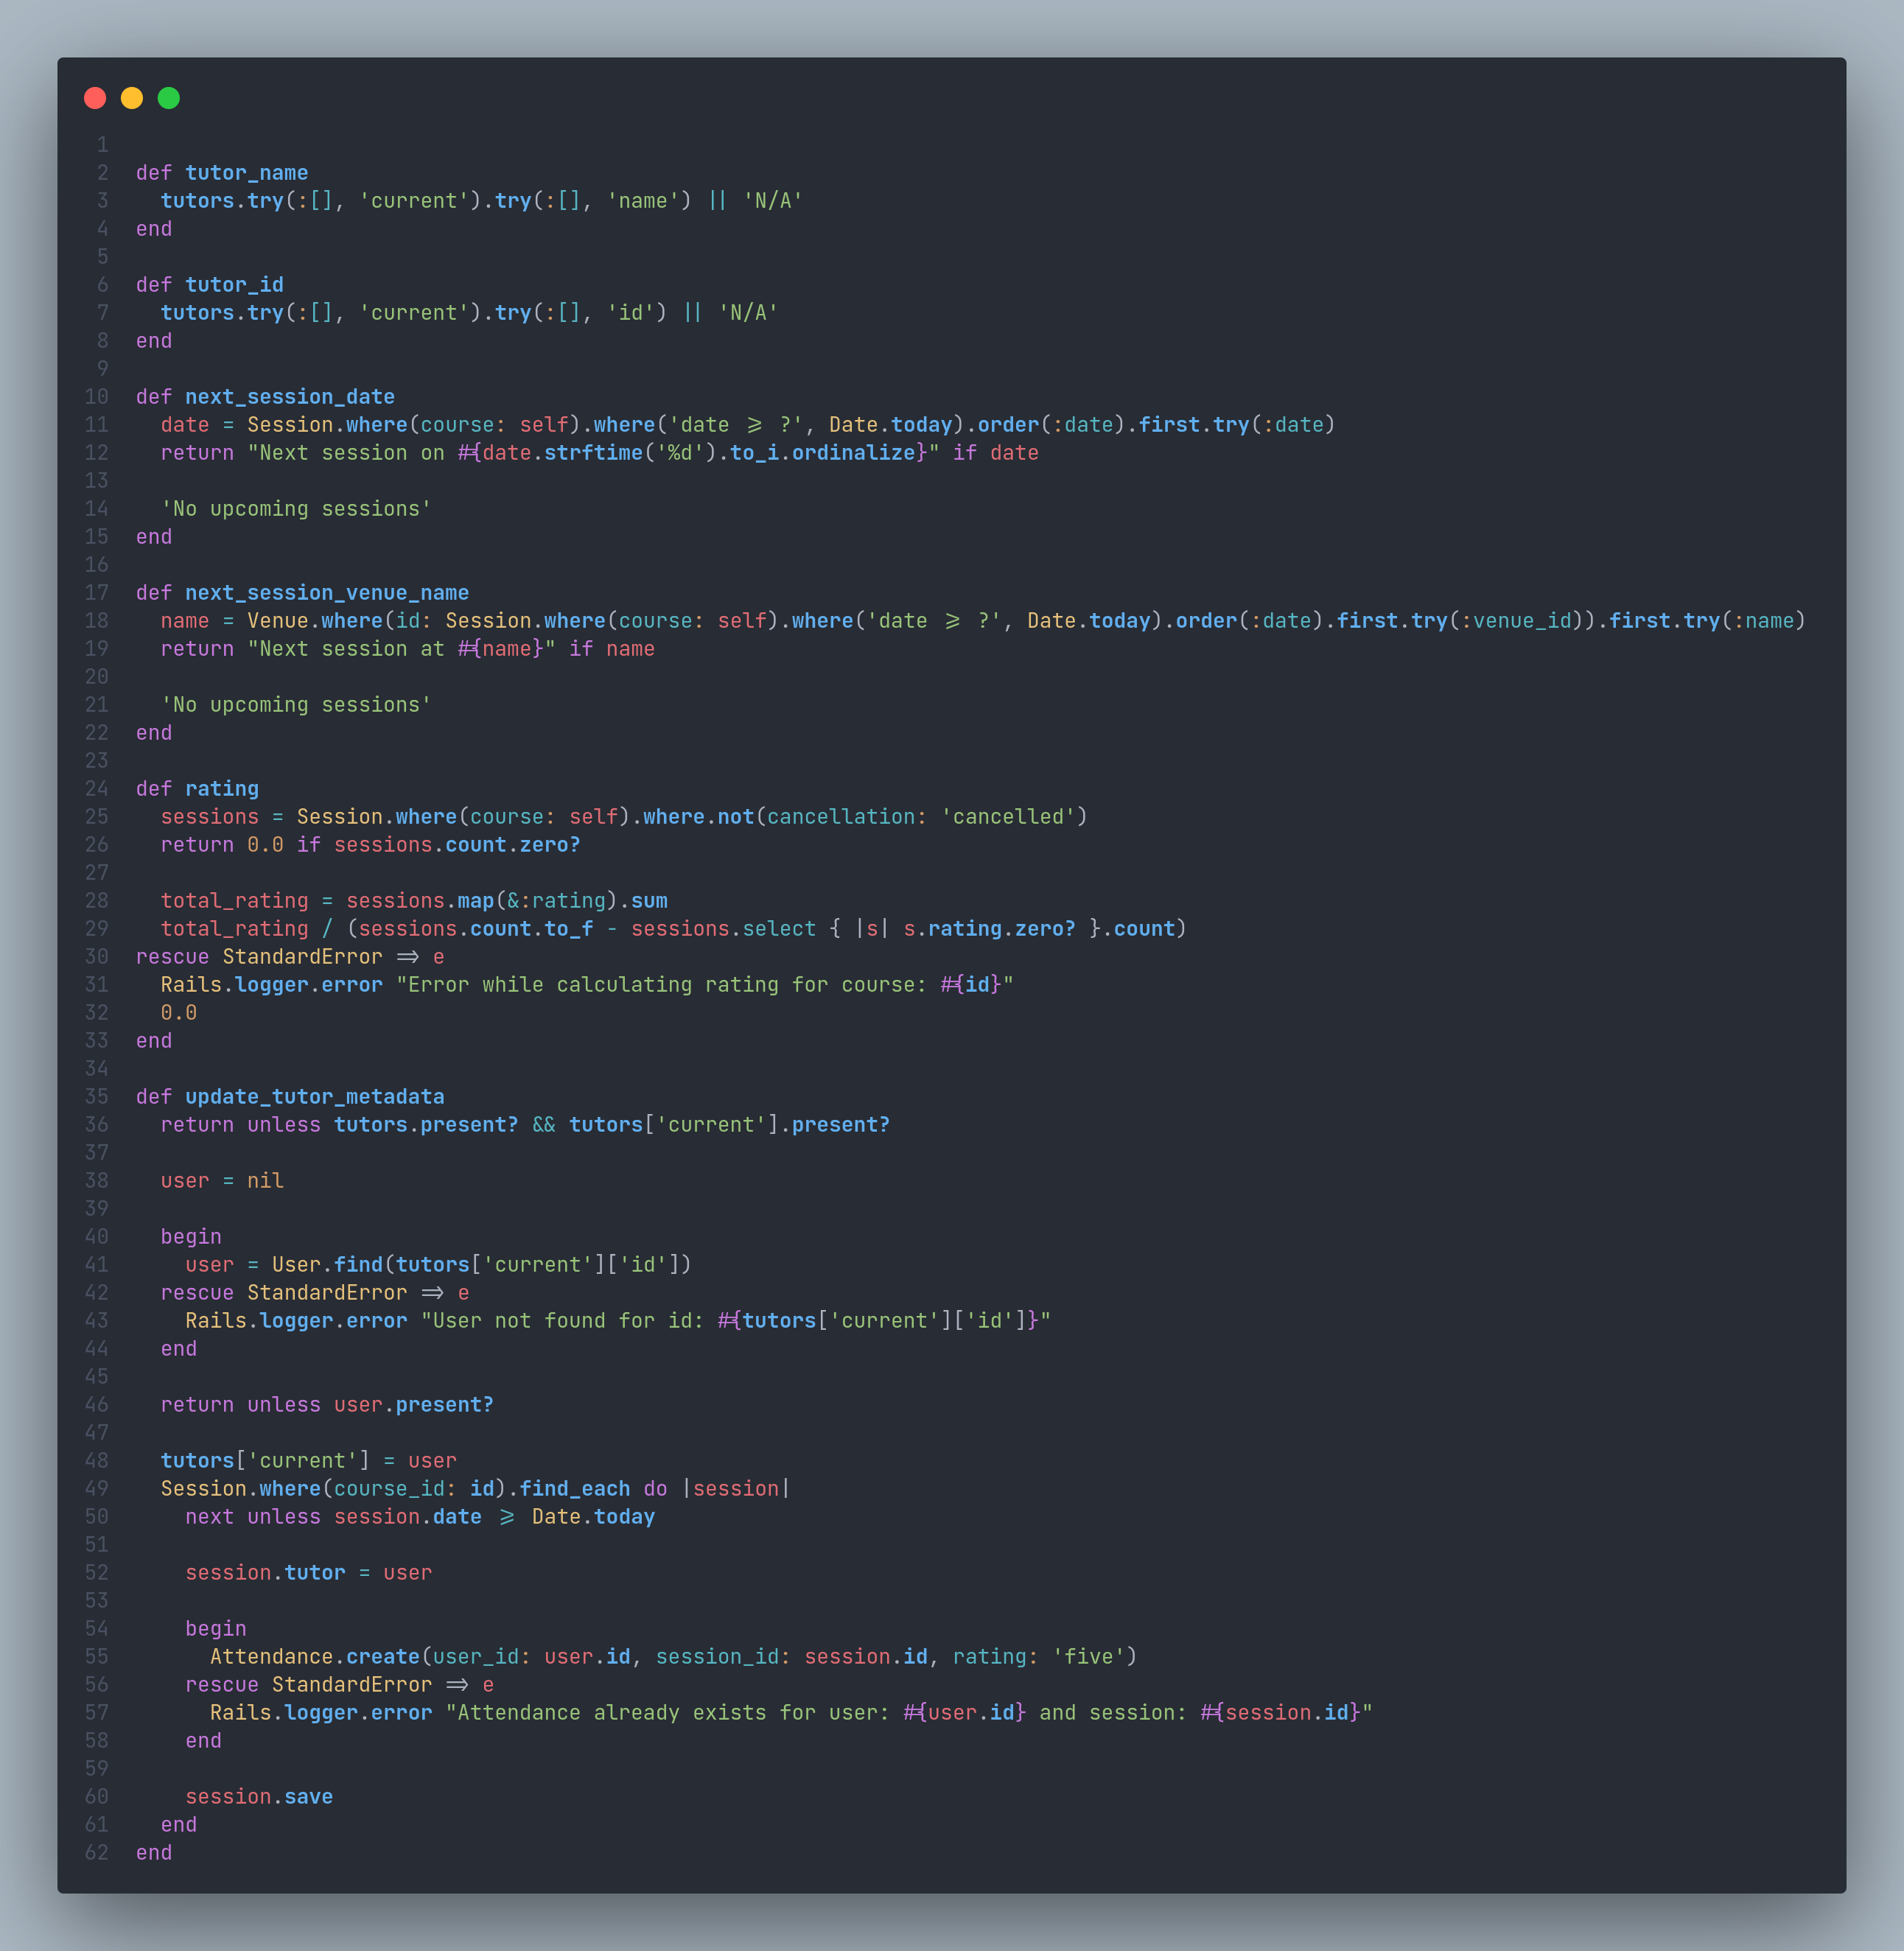
\includegraphics[width=150mm,scale=1]{figures/implementation_and_testing/implementation/backend/course_methods.png}}
            \caption{Course Model - Methods}
        \end{figure}
        
        \vspace{-0.25cm}
        \newendline Now, let's focus on the course model as an example for the rest of the section. The course model represents a specific course within the STDC application. It has attributes such as "name" (representing the name of the course), "status" (indicating the current status of the course), "tutors" (containing information about the course's tutors), and "created\_at" and "updated\_at" (representing timestamps for when the course was created and last updated).
        
        \begin{figure}[H]
            \centerline{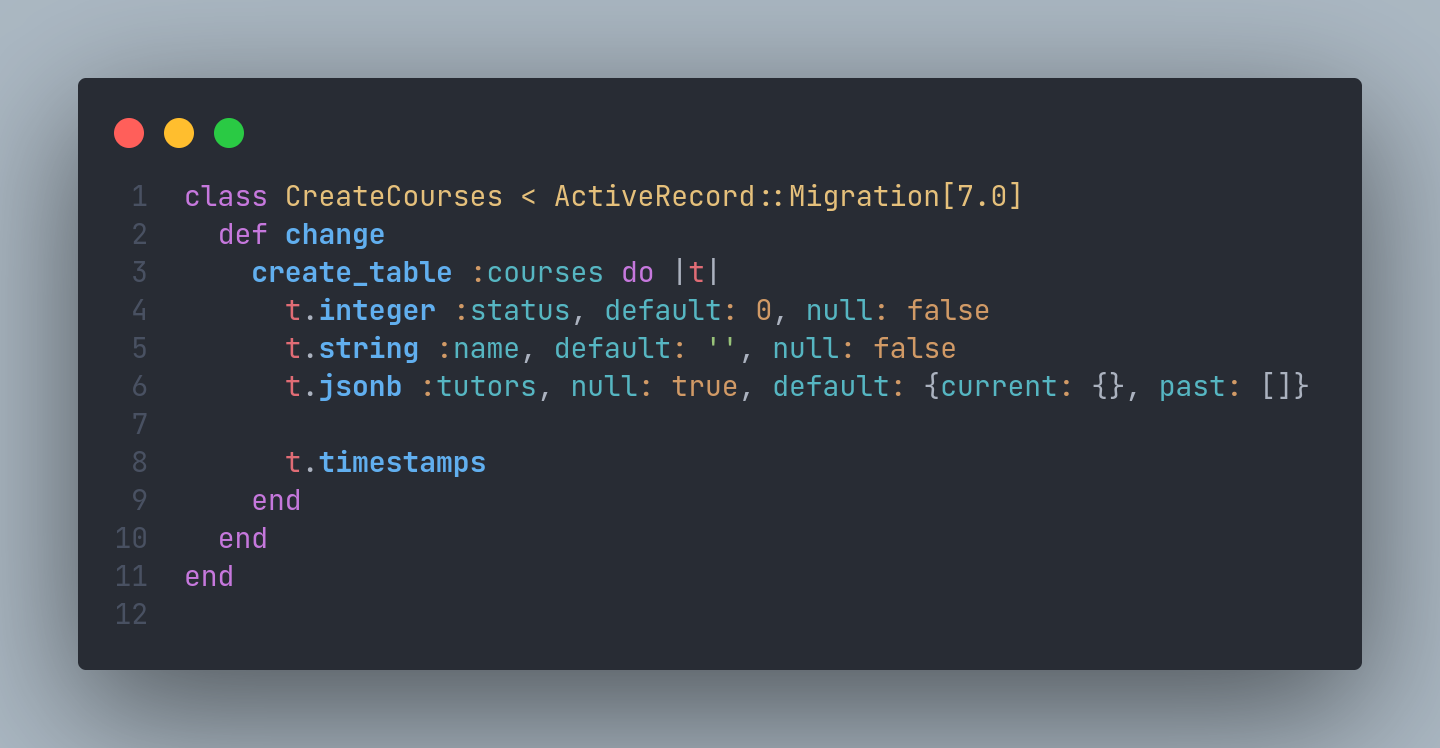
\includegraphics[width=150mm,scale=1]{figures/implementation_and_testing/implementation/backend/course_migrations.png}}
            \caption{Course Model - Migration File}
        \end{figure}

        \vspace{0.25cm}
        \newendline In terms of associations, the course model has several. It includes a "has\_many :enrollments" association, establishing a one-to-many relationship with the Enrollment model. This allows a course to have multiple enrollments, and the "dependent: :destroy" option ensures that associated enrollments are destroyed when the course is destroyed. Additionally, the course model has associations with the User and Session models through enrollments.
        
        \begin{figure}[H]
            \centerline{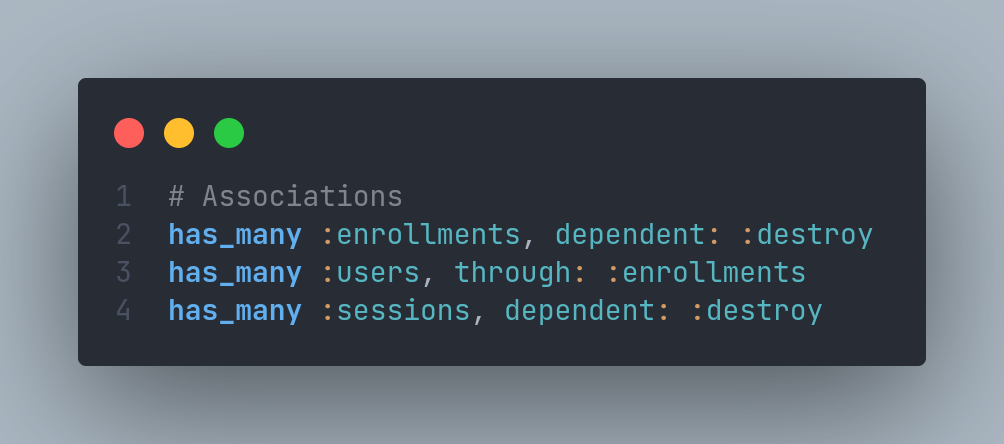
\includegraphics[width=150mm,scale=1]{figures/implementation_and_testing/implementation/backend/course_associations.png}}
            \caption{Course Model - Associations}
        \end{figure}

        \vspace{0.25cm}
        \newendline The course model also utilizes various validations to ensure data consistency. For instance, it includes a presence validation for the "name" attribute, guaranteeing that the name is not empty. Another validation, "validate\_enum\_attribute :status," ensures that the status is present in the model. These validations help maintain the integrity of the data stored in the course model.
        
        \begin{figure}[H]
            \centerline{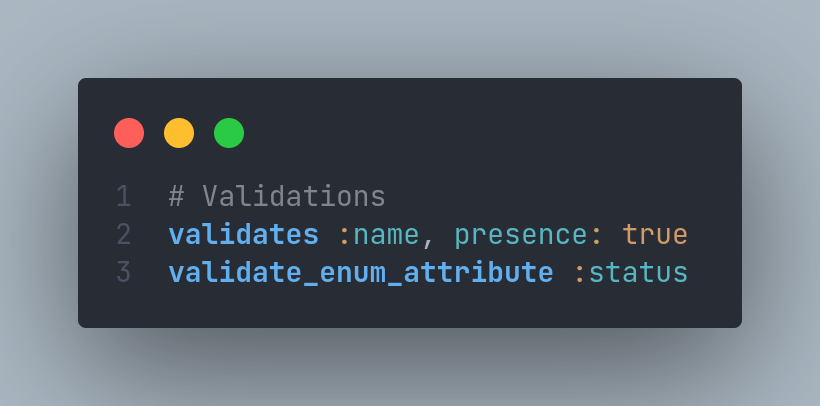
\includegraphics[width=150mm,scale=1]{figures/implementation_and_testing/implementation/backend/course_validations.png}}
            \caption{Course Model - Validations}
        \end{figure}

        \vspace{0.25cm}
        \newendline Additionally, the course model employs callbacks, which are methods called at specific points in the model's lifecycle. For example, the model have an "after\_save" callback that triggers the "update\_tutor\_metadata" method after the model is saved. Another callback, "after\_commit :update\_counter\_cache, on: \%i[create destroy]," updates the counter cache for the model, improving performance by storing the count of the model in the cache.
        
        \begin{figure}[H]
            \centerline{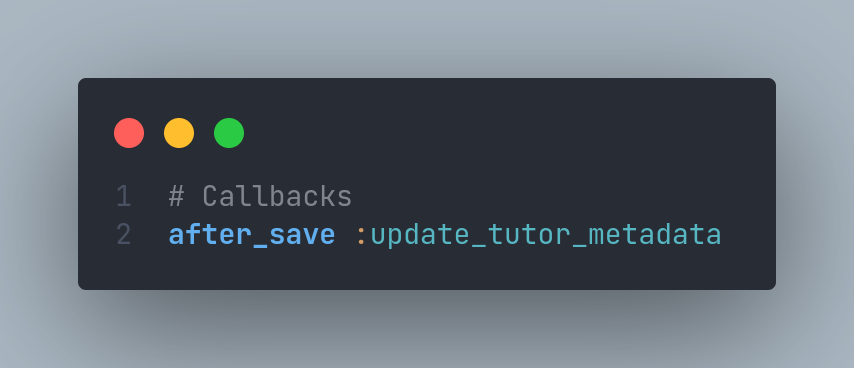
\includegraphics[width=150mm,scale=1]{figures/implementation_and_testing/implementation/backend/course_callbacks.png}}
            \caption{Course Model - Callback}
        \end{figure}

        \begin{figure}[H]
            \centerline{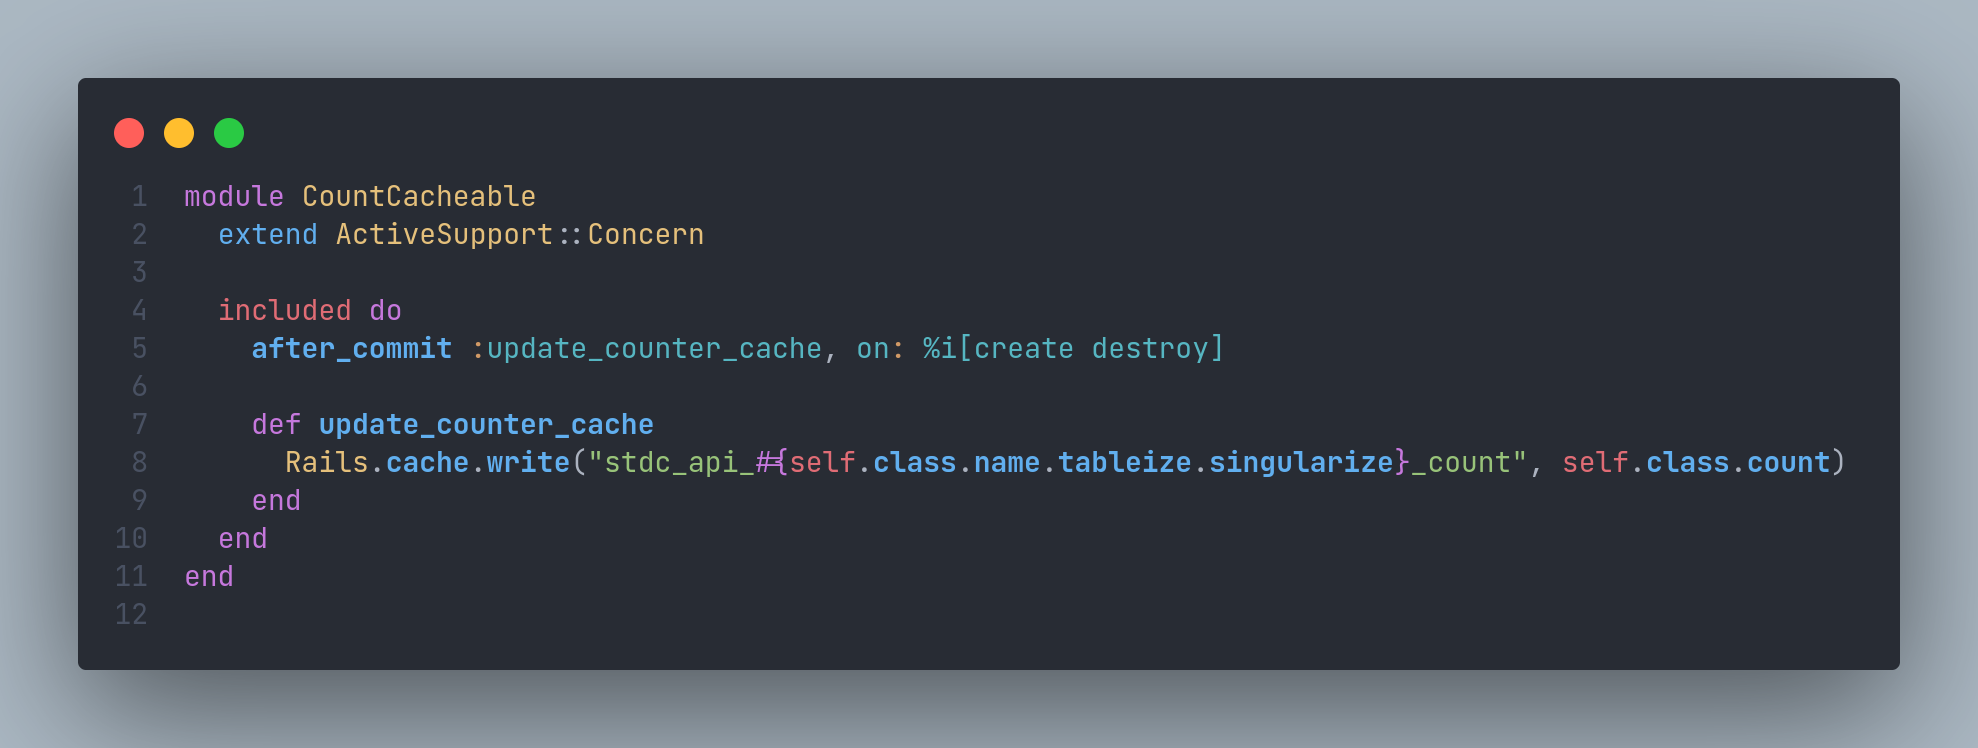
\includegraphics[width=150mm,scale=1]{figures/implementation_and_testing/implementation/backend/course_count_concern.png}}
            \caption{Course Model - Count Cachable Concern}
        \end{figure}

        \vspace{0.25cm}
        \newendline Scopes in the course model provide named queries that allow for flexible and efficient filtering of model instances. For example, a "status" scope could filter courses by their status, while a "by\_name" scope could filter courses by their name. These scopes simplify querying and provide a concise way to retrieve specific subsets of courses based on predefined criteria.
        
        \begin{figure}[H]
            \centerline{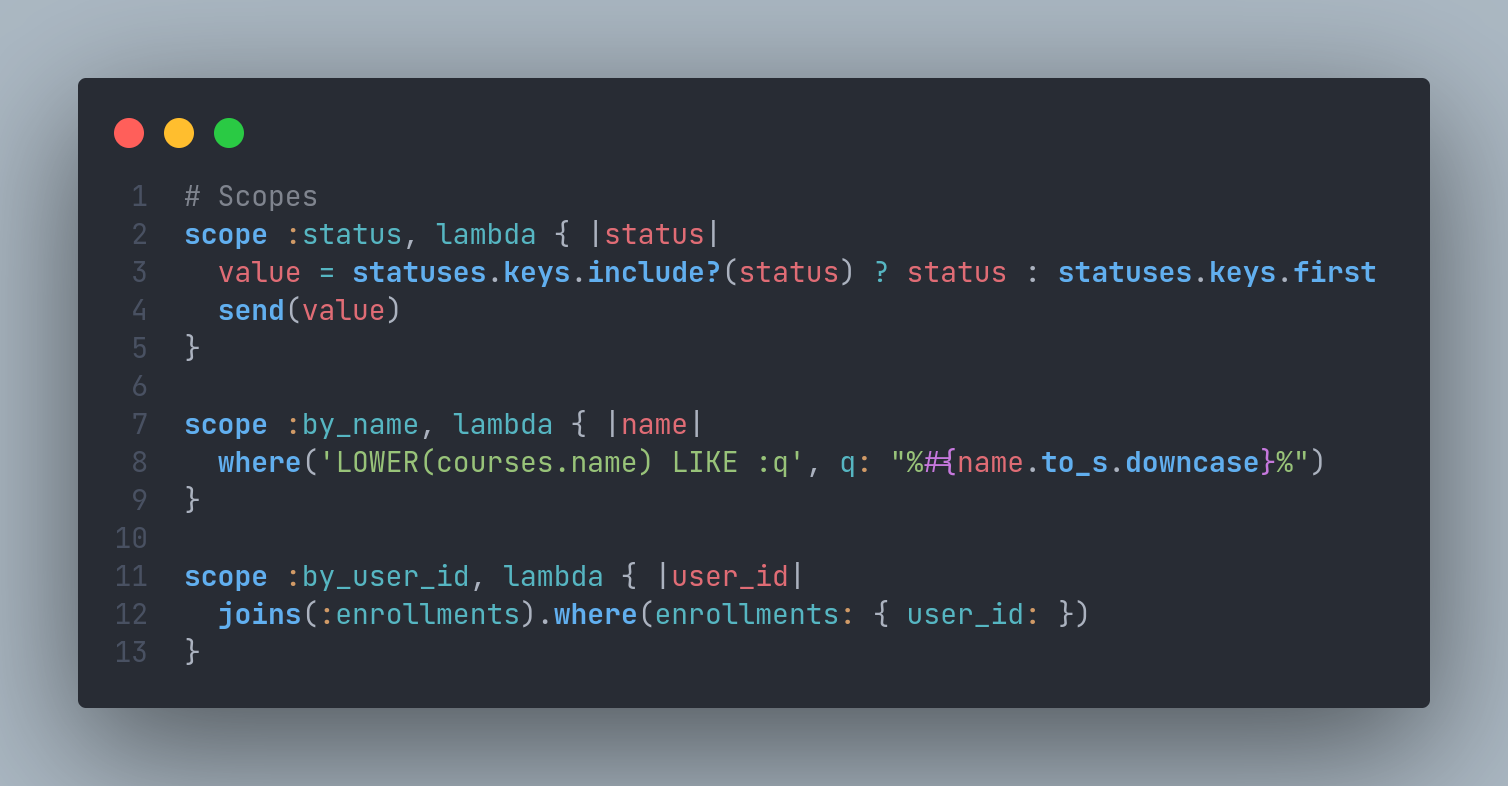
\includegraphics[width=150mm,scale=1]{figures/implementation_and_testing/implementation/backend/course_scopes.png}}
            \caption{Course Model - Scopes}
        \end{figure}

        \vspace{0.25cm}
        \newendline By utilizing these components such as validations, enums, methods, callbacks, associations, and scopes, the course model in the STDC application ensures data consistency, enables efficient querying and filtering, defines relationships with other models, and encapsulates essential behaviors and business logic.

    \clearpage

    
%%%%%%%%%%%%%%%%%%%%%%%%%%%%%%%%%%%%%%%%%%%%%%%%%%%%%%%%%%%%%%%%%%
%%%%%%%%%%%%%%%%%%%%%%%%%%%%%%%%%%%%%%%%%%%%%%%%%%%%%%%%%%%%%%%%%%
%%%%%%%%%%%%%%%%%%%%%%%%%%%%%%%%%%%%%%%%%%%%%%%%%%%%%%%%%%%%%%%%%%
%%%%%%%%%%%%%%%%%%%%%%%%%%%%%%%%%%%%%%%%%%%%%%%%%%%%%%%%%%%%%%%%%%

    \vspace{0.25cm}
    \newendline \textbf{\textit{Controller}}\newendline
    The following is a detailed explanation of the controllers used in the Student Talent Development Center (STDC) web application. Even though not all of the controllers will be mentioned, a through explanation of how one of the controllers work with their dependencies will be provided.

    \vspace{0.25cm}
    \newendline The STDC web application has a total of 10 controllers, which are as follows:
        
    \begin{itemize}
        \item ApplicationController
        \item GuardController
        \item AttendancesController
        \item CoursesController
        \item FeedbacksController
        \item MaterialsController
        \item QuestionsController
        \item SessionsController
        \item VenuesController
        \item UsersController
    \end{itemize}

    \vspace{0.25cm}
    \newendline The ApplicationController is the base controller for all the other controllers. It is inherited by the GuardController which is the parent of all the other controllers. In the ApplicationController the following modules are included:

    \begin{figure}[H]
        \centerline{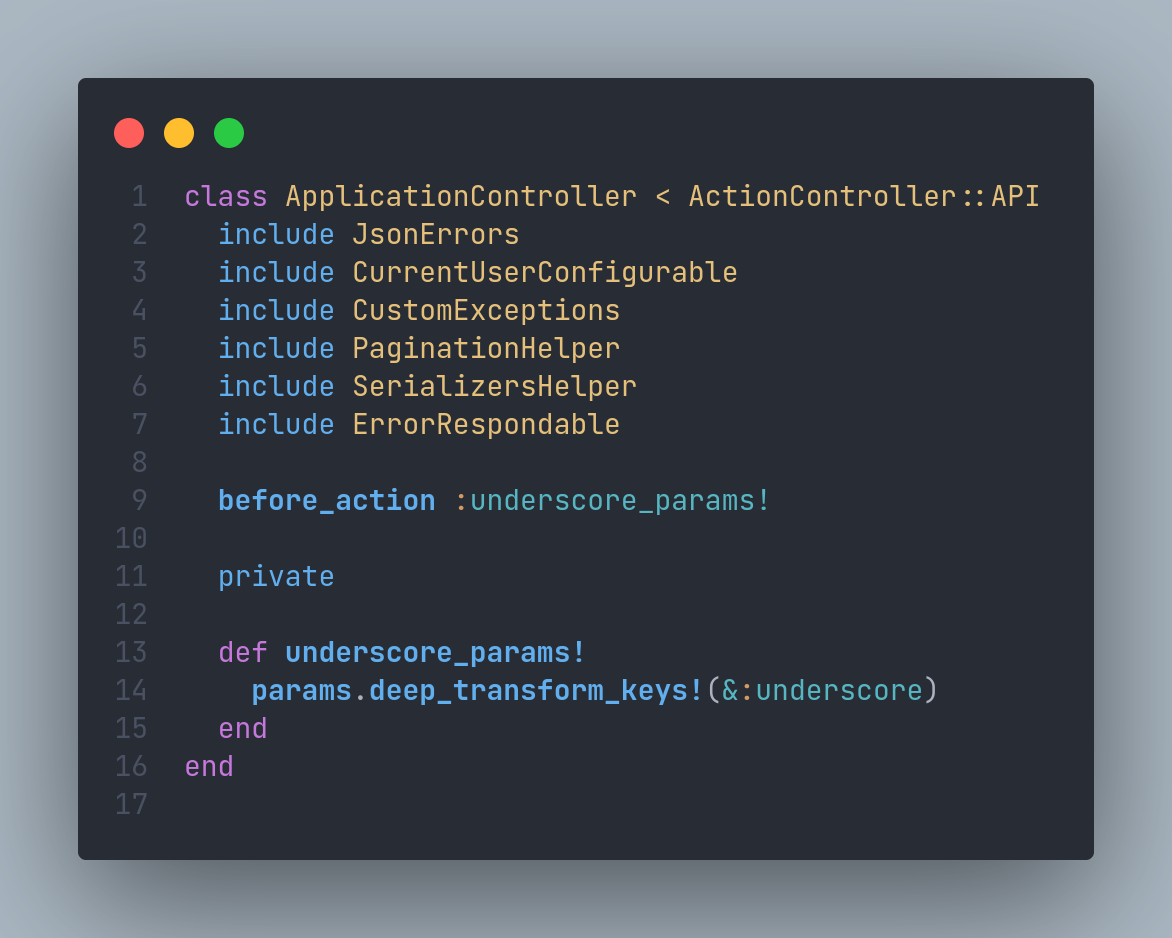
\includegraphics[width=150mm,scale=1]{figures/implementation_and_testing/implementation/backend/application_controller.png}}
        \caption{ApplicationController}
    \end{figure}

    \begin{itemize}
        \item JsonErrors: This module is responsible for handling the errors that occur in the controllers.
        \item CurrentUserConfigurable: This module is responsible for configuring the current user by setting the current user after the user has been authenticated.
        \item CustomExceptions: This module is responsible for defining the custom exceptions that are used in the controllers.
        \item PaginationHelper: This module is responsible for handling the pagination of the resources.
        \item SerializersHelper: This module is responsible for handling the serialization of the resources.
        \item ErrorRespondable: This module is responsible for formatting the errors that occur in the controllers.
    \end{itemize}

    \vspace{0.25cm}
    \newendline The ApplicationController has a method called underscore\_params! which is responsible for transforming the keys of the params hash to underscore. This is done to ensure that the keys of the params hash are in the correct format of snake case before they are used in the controllers.

    \vspace{0.25cm}
    \newendline The GuardController has been mentioned prior to this section, therefore, we will not discuss it again. Now, let's dive into the Crudable and the CoursesController as an example.

    \vspace{0.25cm}
    \newendline The Crudable module is responsible for defining the CRUD actions for the controllers. The Crudable module is developed using Template Method design pattern. The Crudable module is included in the other controllers to define the CRUD actions for the controllers.

    \begin{figure}[H]
        \centerline{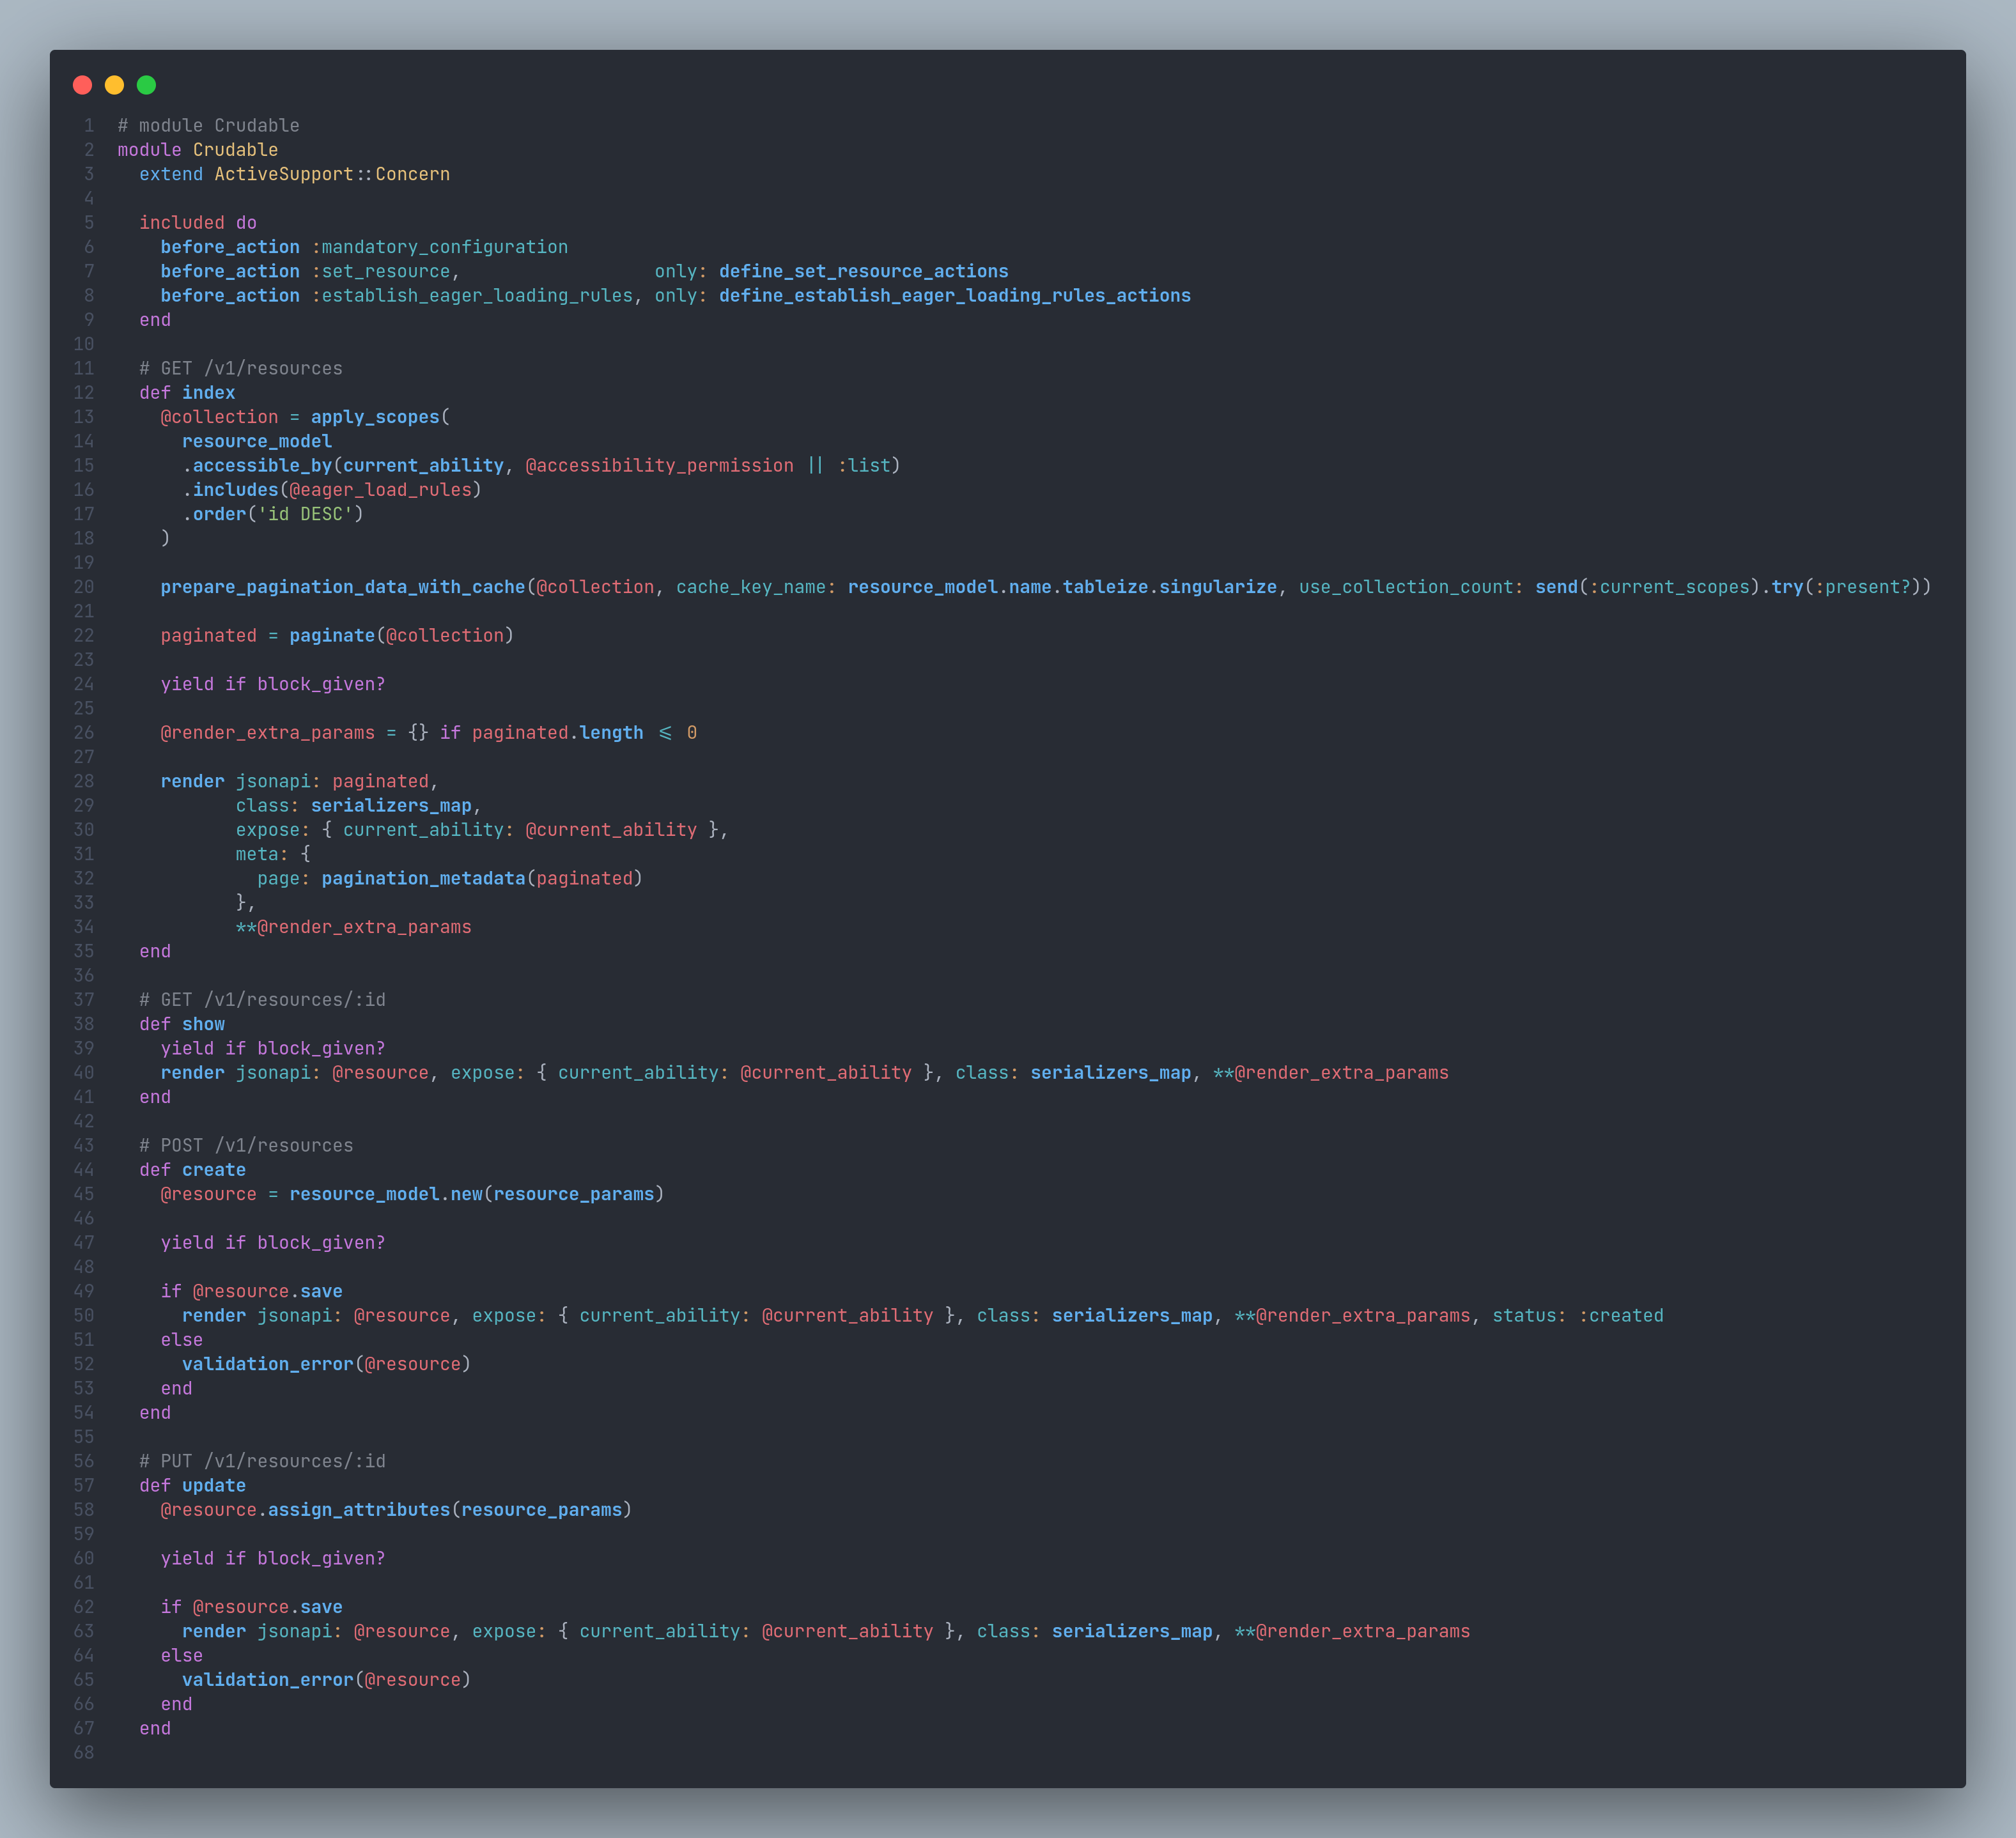
\includegraphics[width=150mm,scale=1]{figures/implementation_and_testing/implementation/backend/curdable-1.png}}
        \caption{Crudable - Part 1}
    \end{figure}


    \begin{figure}[H]
        \centerline{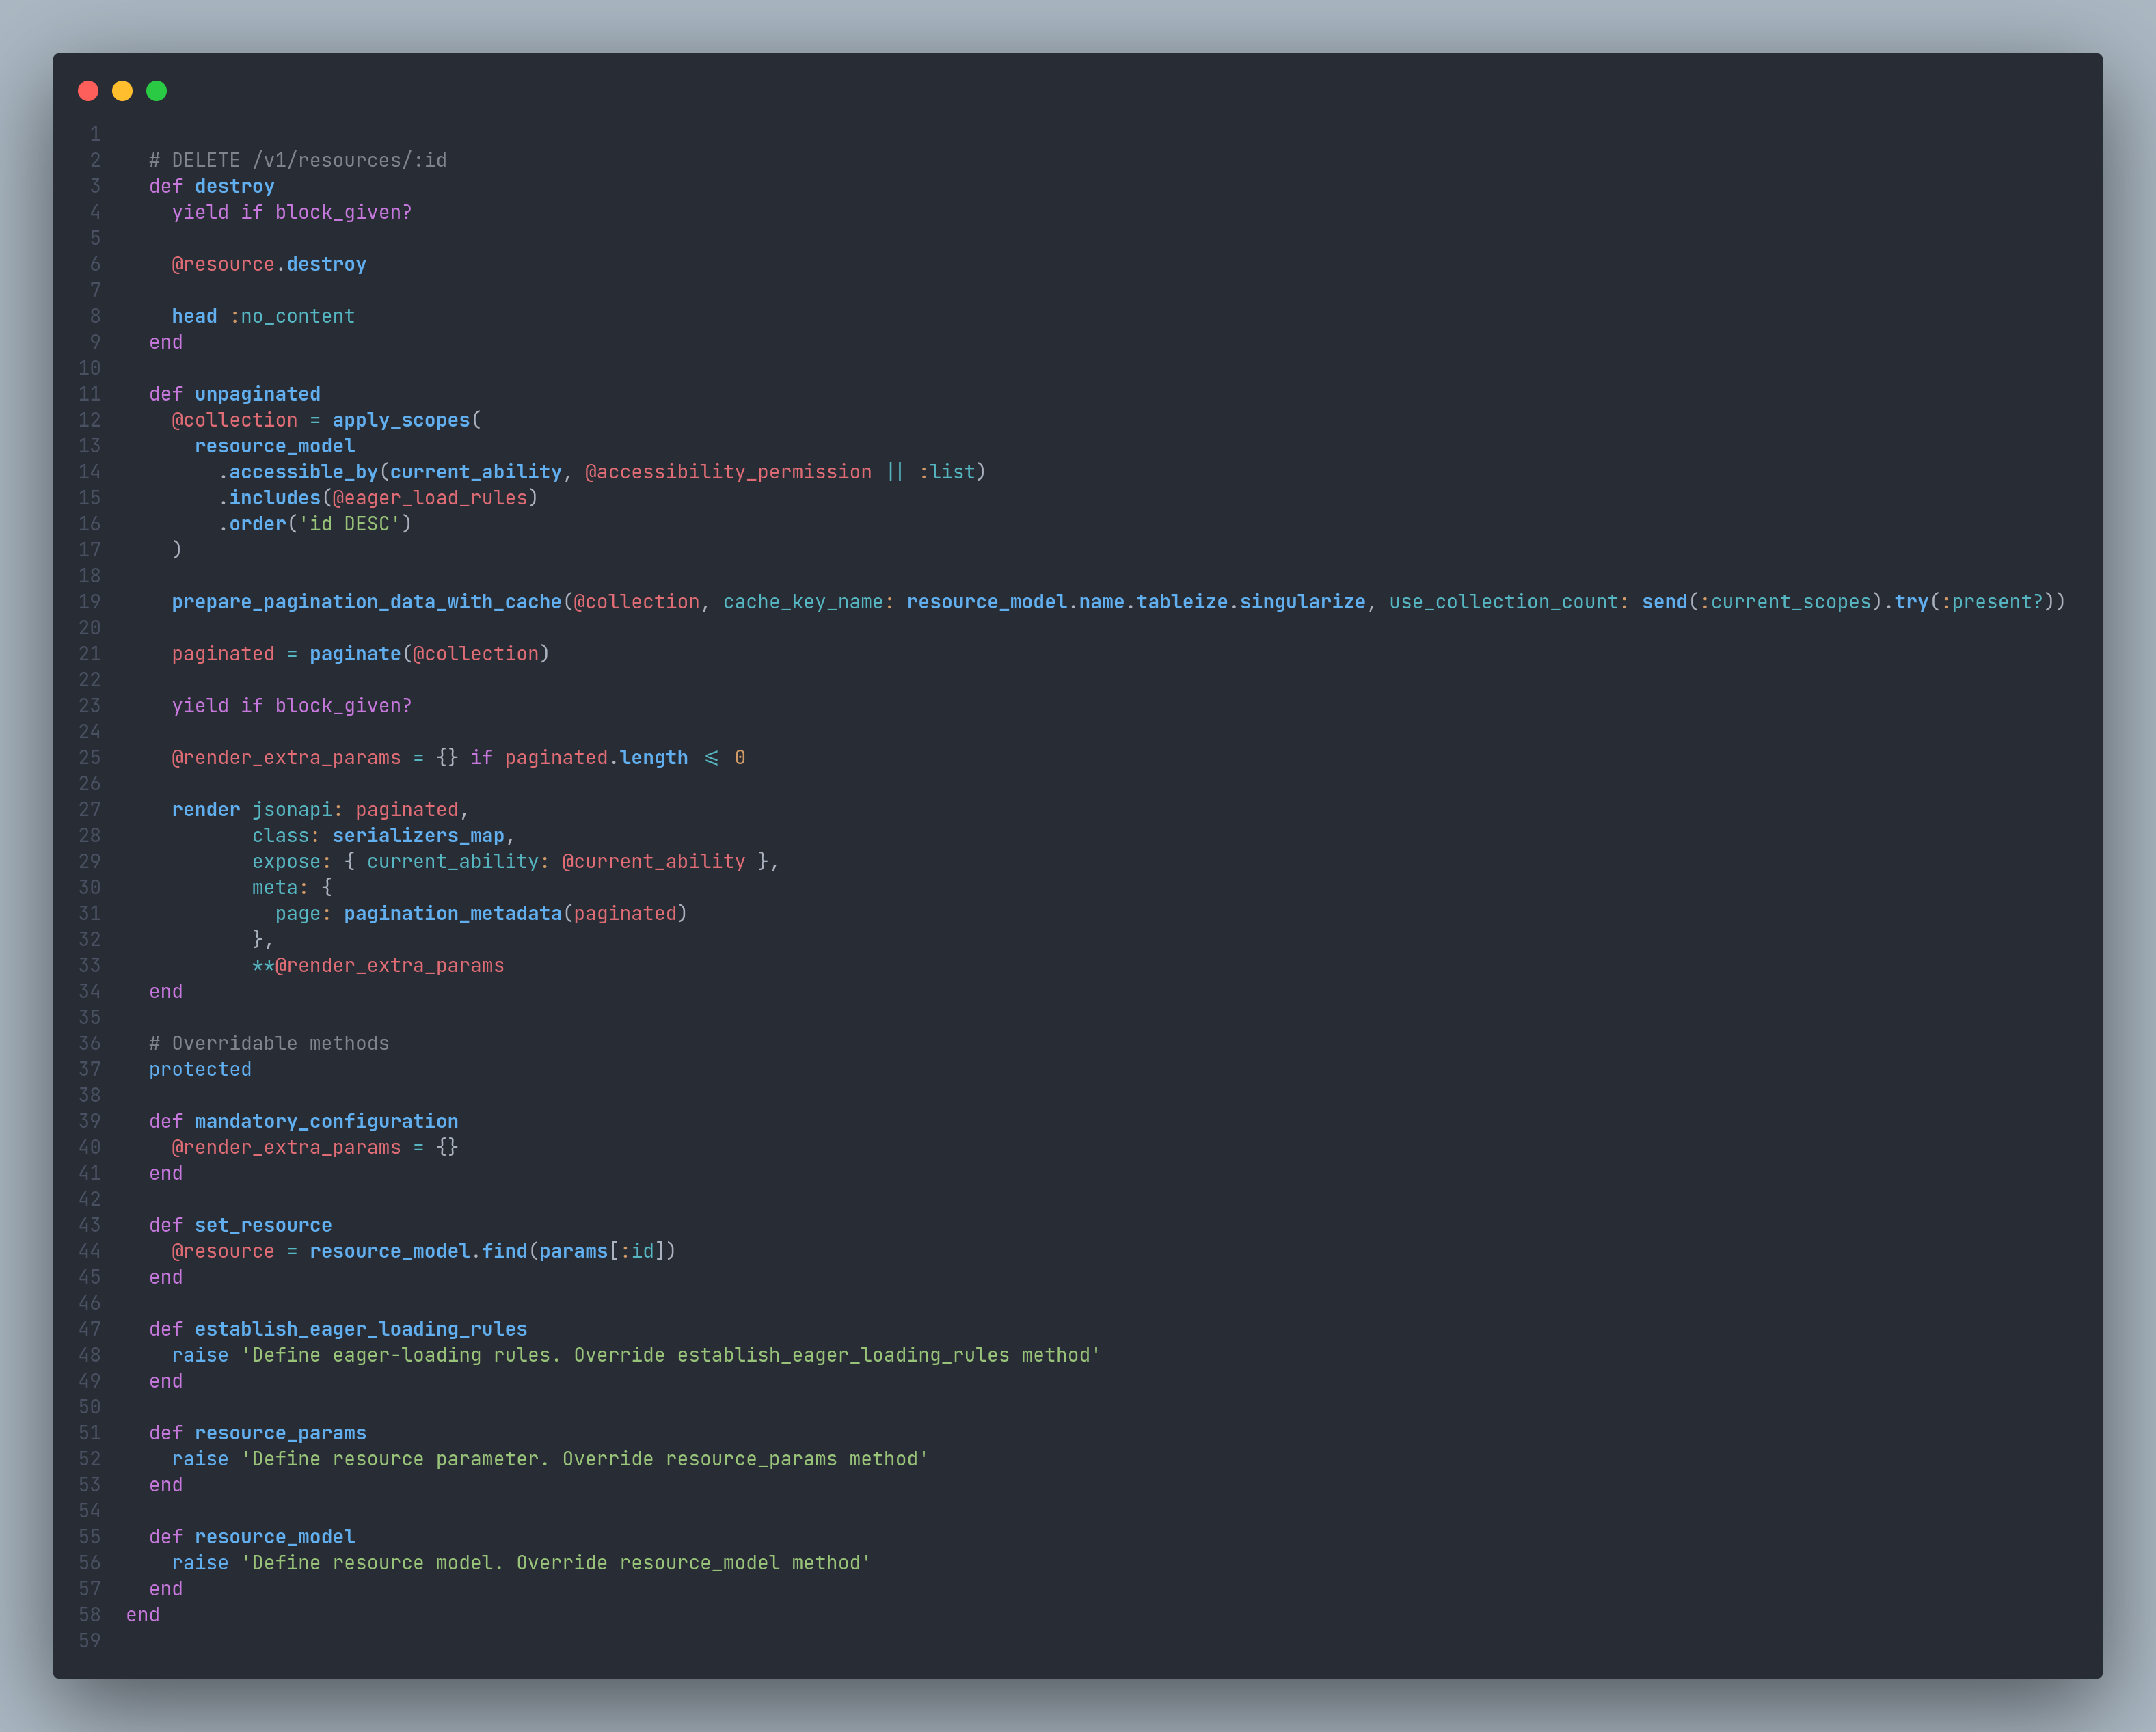
\includegraphics[width=150mm,scale=1]{figures/implementation_and_testing/implementation/backend/curdable-2.png}}
        \caption{Crudable - Part 2}
    \end{figure}

    \vspace{0.25cm}
    \newendline The Crudable requires the following methods to be defined in the controllers that include it:

    \begin{itemize}
        \item mandatory\_configuration: This method is responsible for defining the mandatory configuration for the controller.
        \item set\_resource: This method is responsible for setting the resource for the controller. Finding single resource to be used by other methods such as show and update.
        \item establish\_eager\_loading\_rules: This method is responsible for establishing the eager loading rules for the controller. Eager loading is a concept in Rails that allows you to load all the associated objects of the object you are querying in a single query. This is done to avoid the N+1 query problem.
        \item resource\_params: This method is responsible for defining the resource parameters for the controller. The resource parameters are the parameters that are allowed to be passed to the controller. It is a way to whitelist the parameters that are allowed to be passed to the controller which is a security measure.
        \item resource\_model: This method is responsible for defining the resource model for the controller. The resource model is the model that the controller is responsible for. For example, the CoursesController is responsible for the Course model.
    \end{itemize}

    \vspace{0.25cm}
    \newendline The Crudable also makes use of PaginationHelper and SerializersHelper modules. The PaginationHelper module is responsible for handling the pagination of the resources. The SerializersHelper module is responsible for handling the serialization of the resources. Both of these will map the response to the JSON API specification. More on each will be discussed later. Now, let's take a look at the CoursesController.

    \begin{figure}[H]
        \centerline{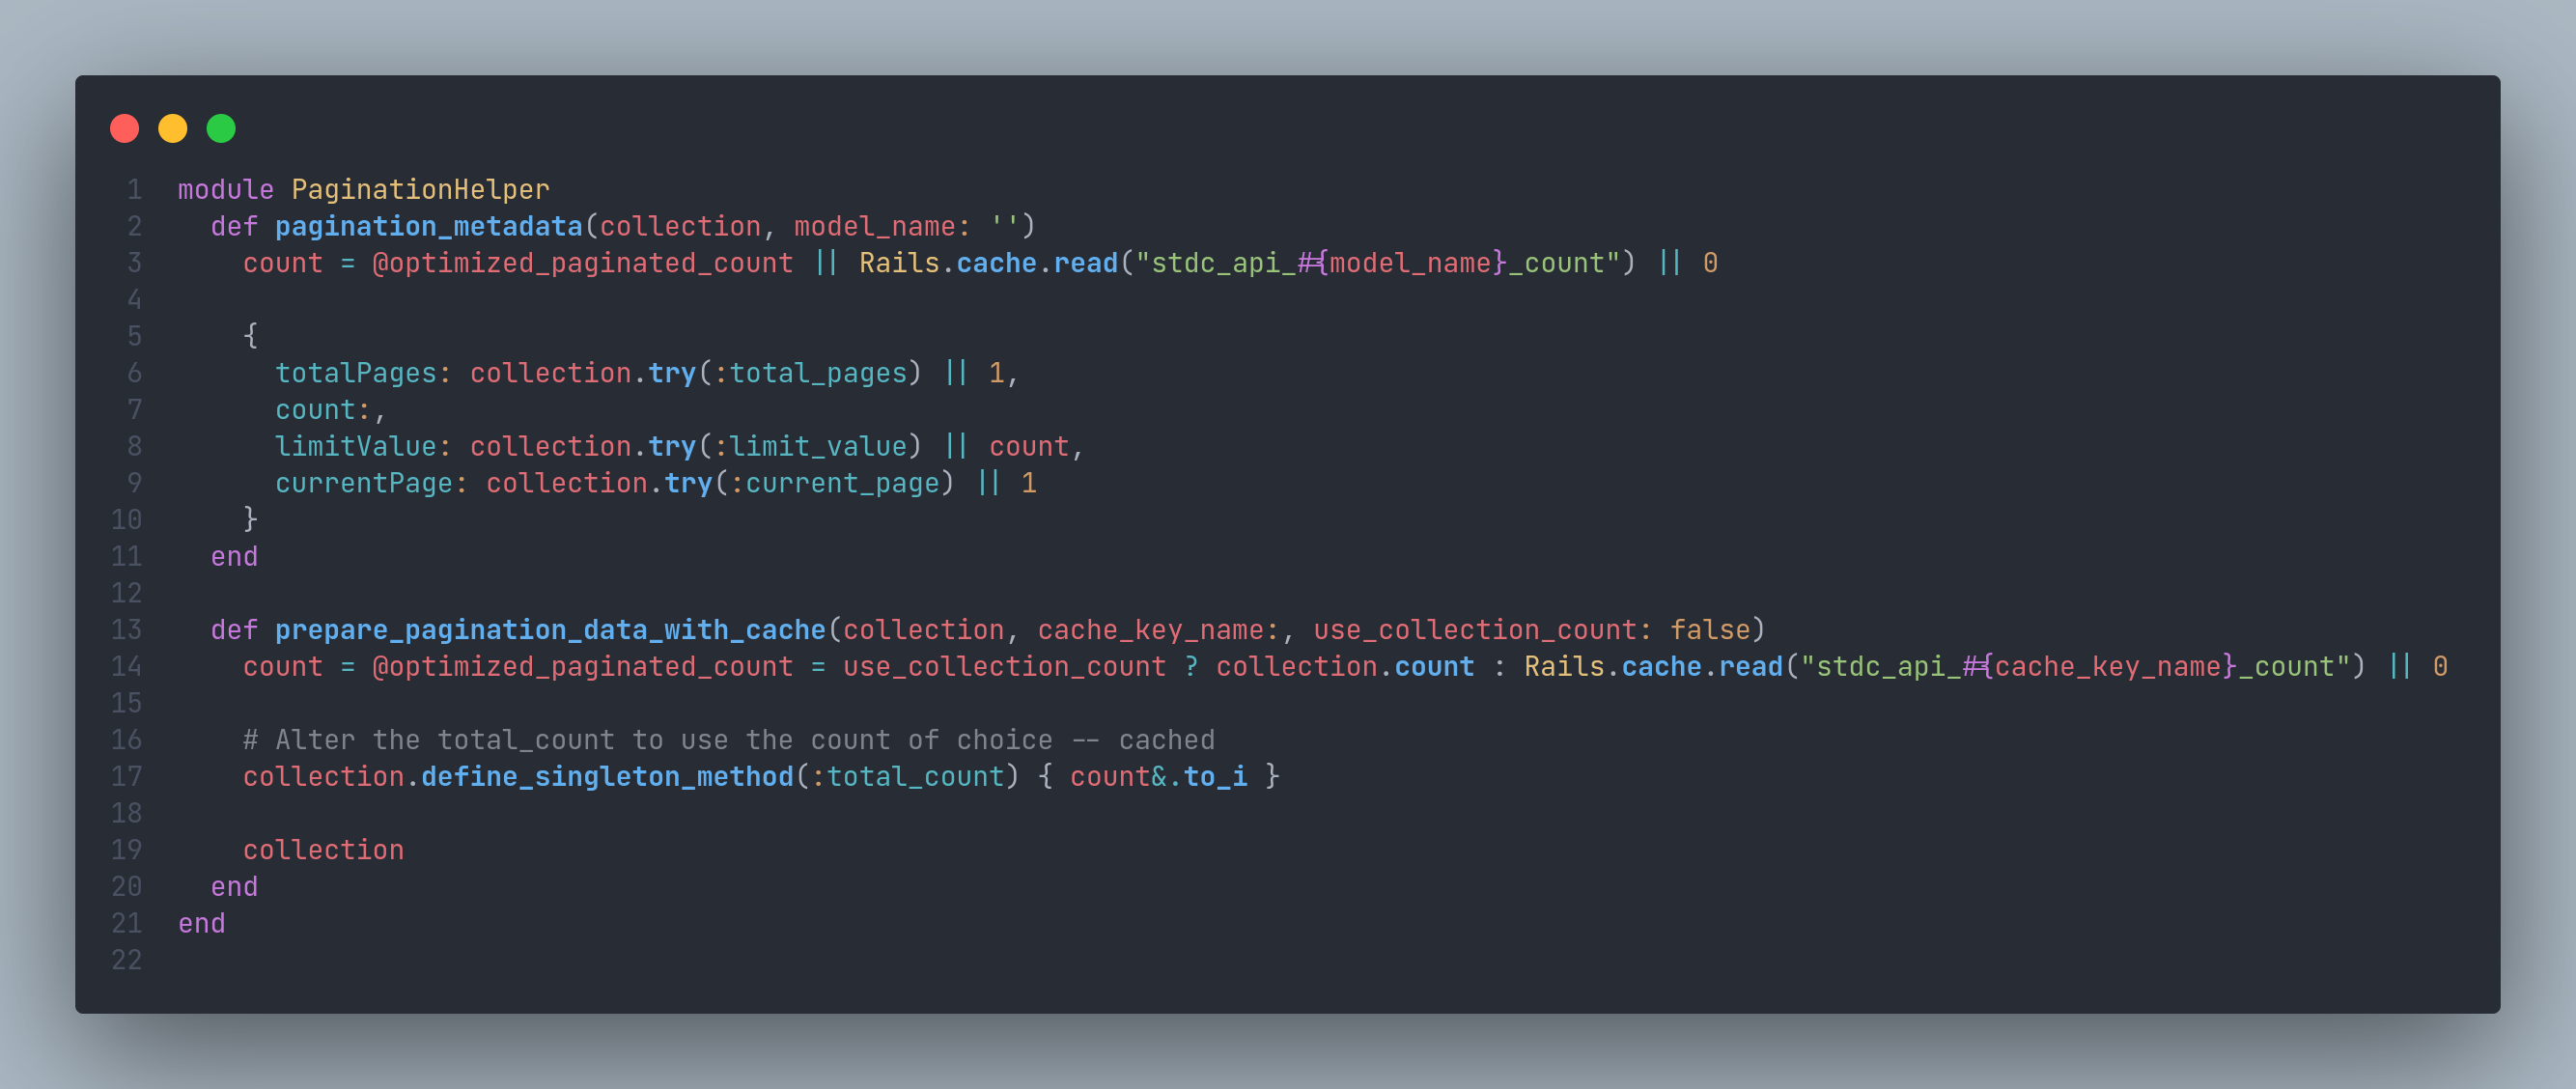
\includegraphics[width=150mm,scale=1]{figures/implementation_and_testing/implementation/backend/pagination_helper.png}}
        \caption{PaginationHelper}
    \end{figure}

    \vspace{0.25cm}
    \newendline The CoursesController is responsible for handling the requests related to the Course model. The CoursesController includes the Crudable module, and it defines the basic CRUD actions for the Course model. The CoursesController also has a few more endpoints defined in it. The CoursesController has the following endpoints defined in it:

    \begin{itemize}
        \item GET /v1/courses: This endpoint is responsible for listing the courses, it is a paginated endpoint which means that it can be filtered, sorted, and paginated.
        \item GET /v1/courses/:id: This endpoint is responsible for showing a specific course.
        \item POST /v1/courses: This endpoint is responsible for creating a new course.
        \item PUT /v1/courses/:id: This endpoint is responsible for updating a specific course.
        \item DELETE /v1/courses/:id: This endpoint is responsible for deleting a specific course.
        \item GET /v1/courses/unpaginated: This endpoint is responsible for listing the courses, it is an unpaginated endpoint which means that it cannot be filtered and sorted.
        \item GET /v1/courses/:id/students: This endpoint is responsible for listing the students of a specific course.
        \item POST /v1/courses/assign\_tutor: This endpoint is responsible for assigning a tutor to a specific course.
    \end{itemize}

    
    \vspace{0.25cm}
    \newendline The CoursesController overrides the create and update methods defined in the Crudable module. The create and update methods are overridden to assign a tutor to the course if the user\_id parameter is passed to the controller.\\

    \begin{figure}[H]
        \centerline{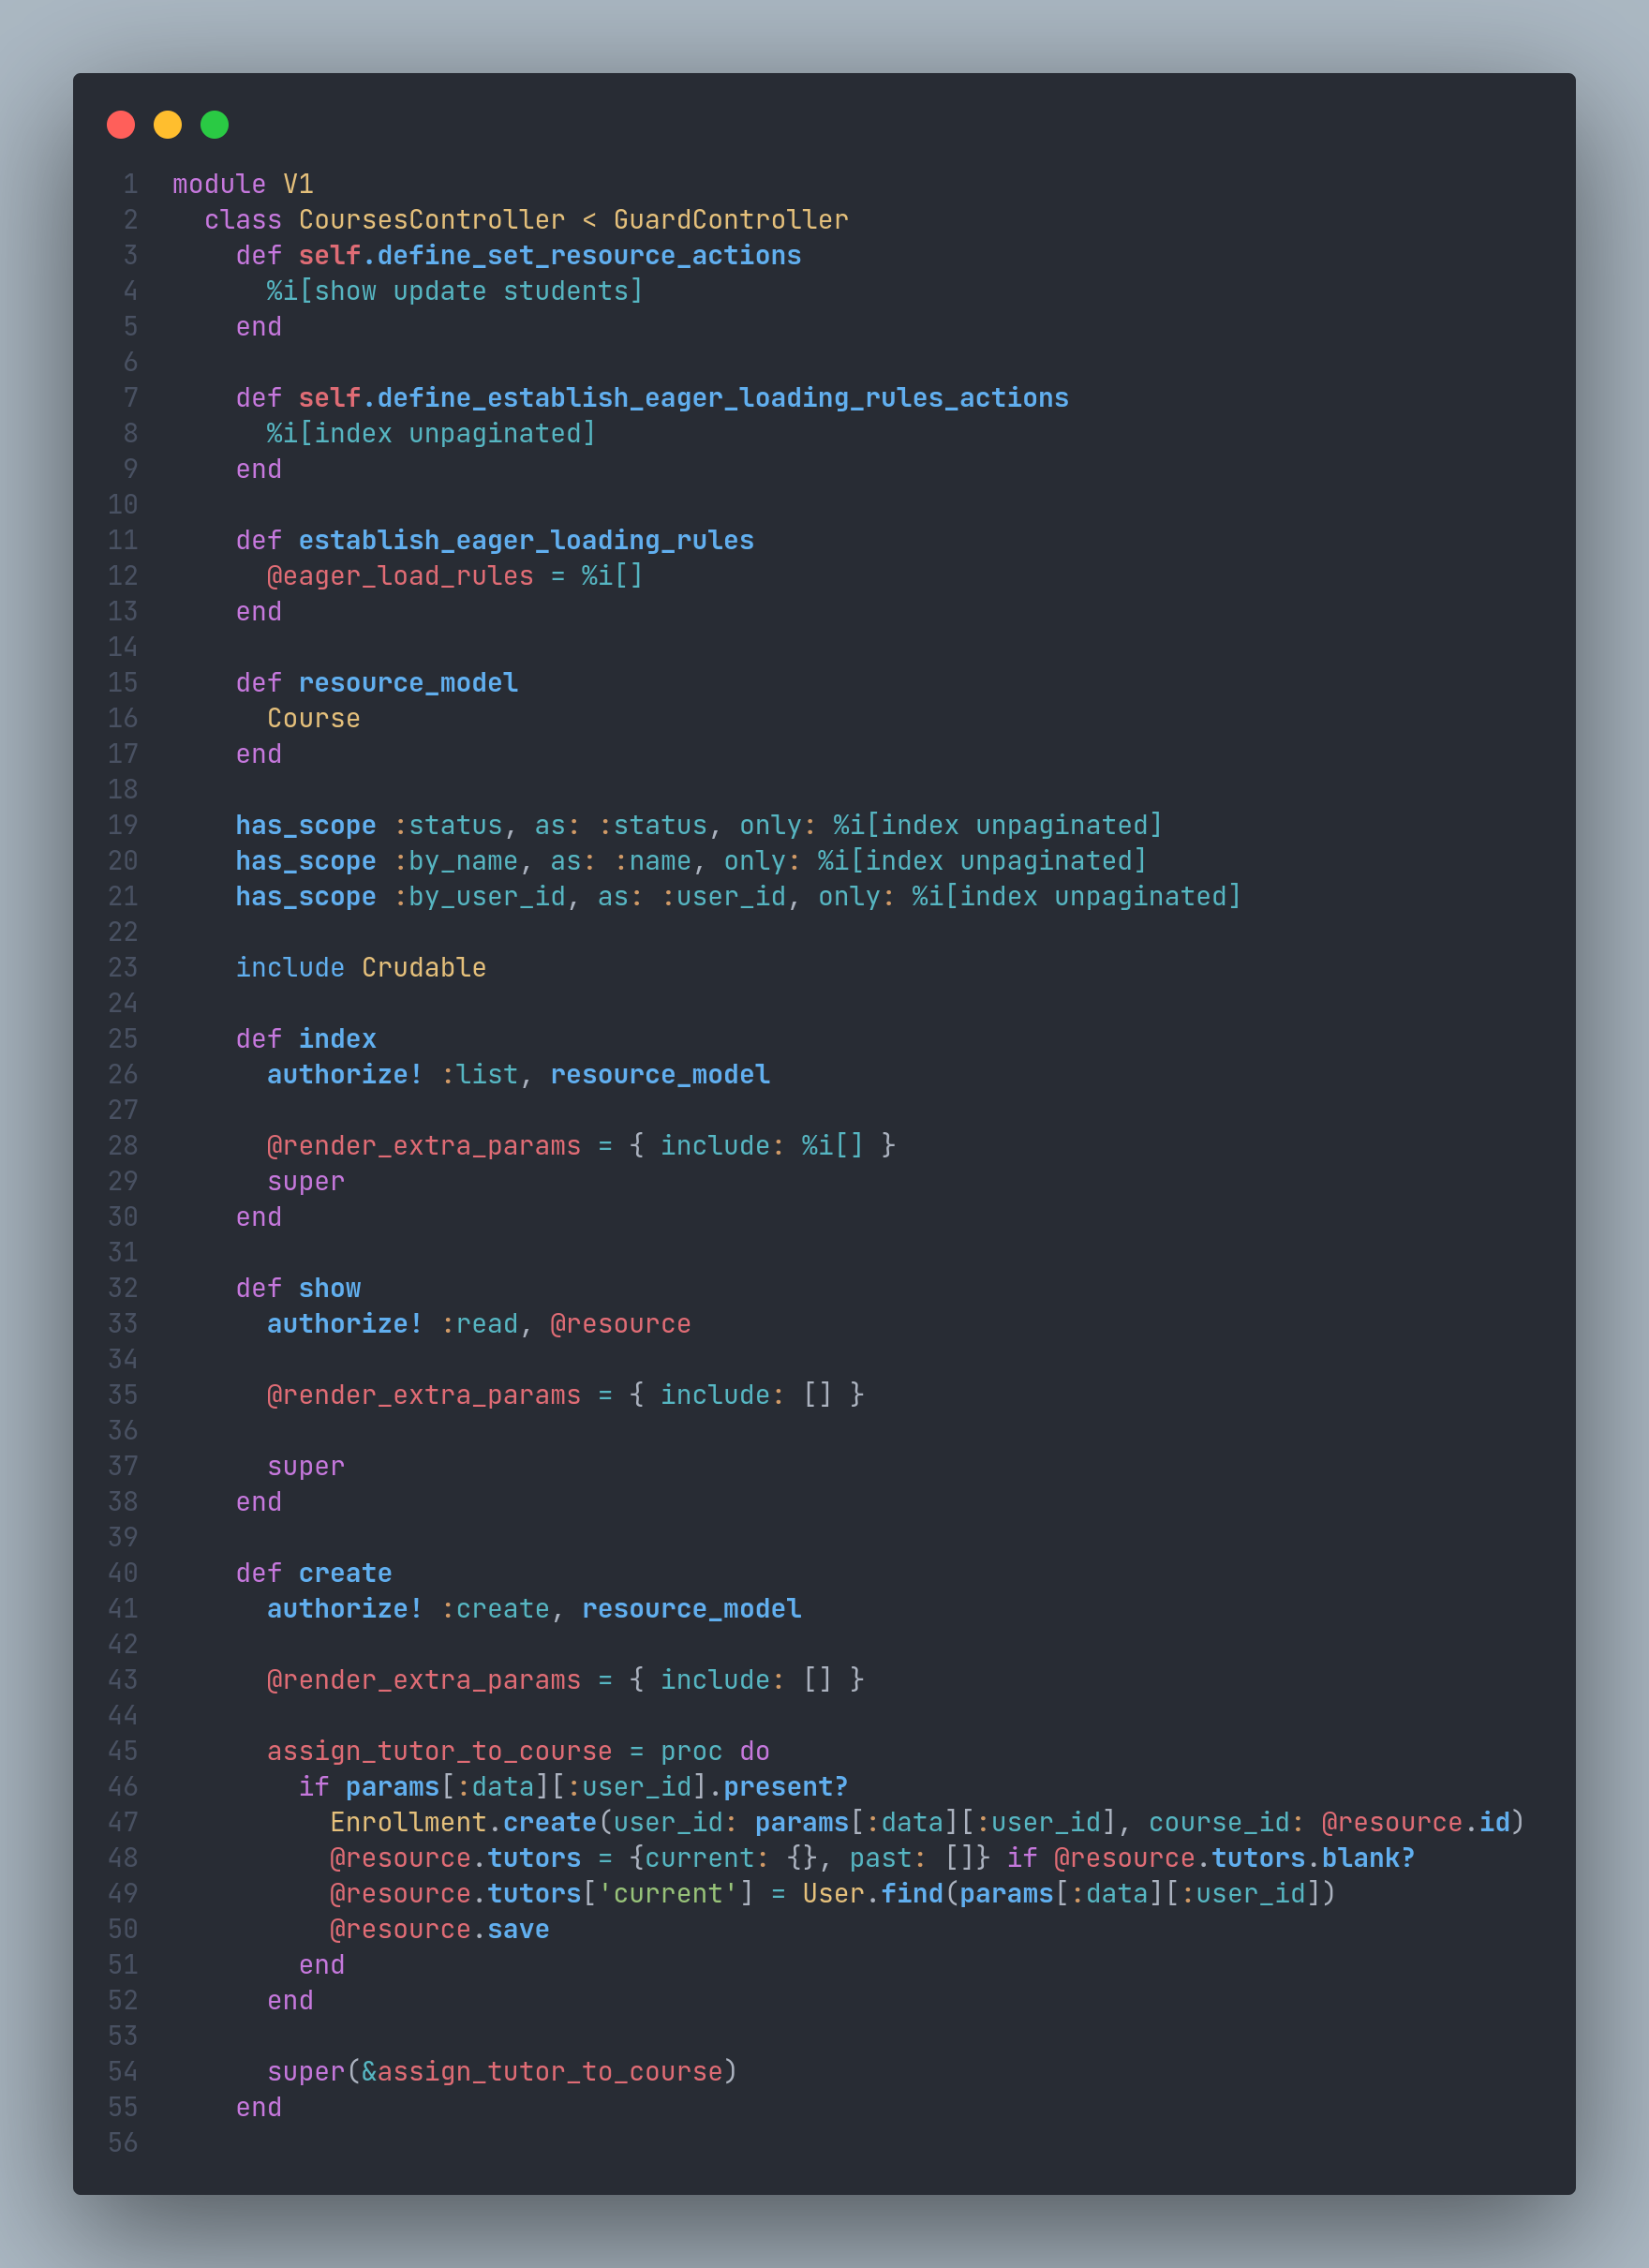
\includegraphics[width=150mm,scale=1]{figures/implementation_and_testing/implementation/backend/courses_controller-1.png}}
        \caption{CoursesController - Part 1}
    \end{figure}

    \begin{figure}[H]
        \centerline{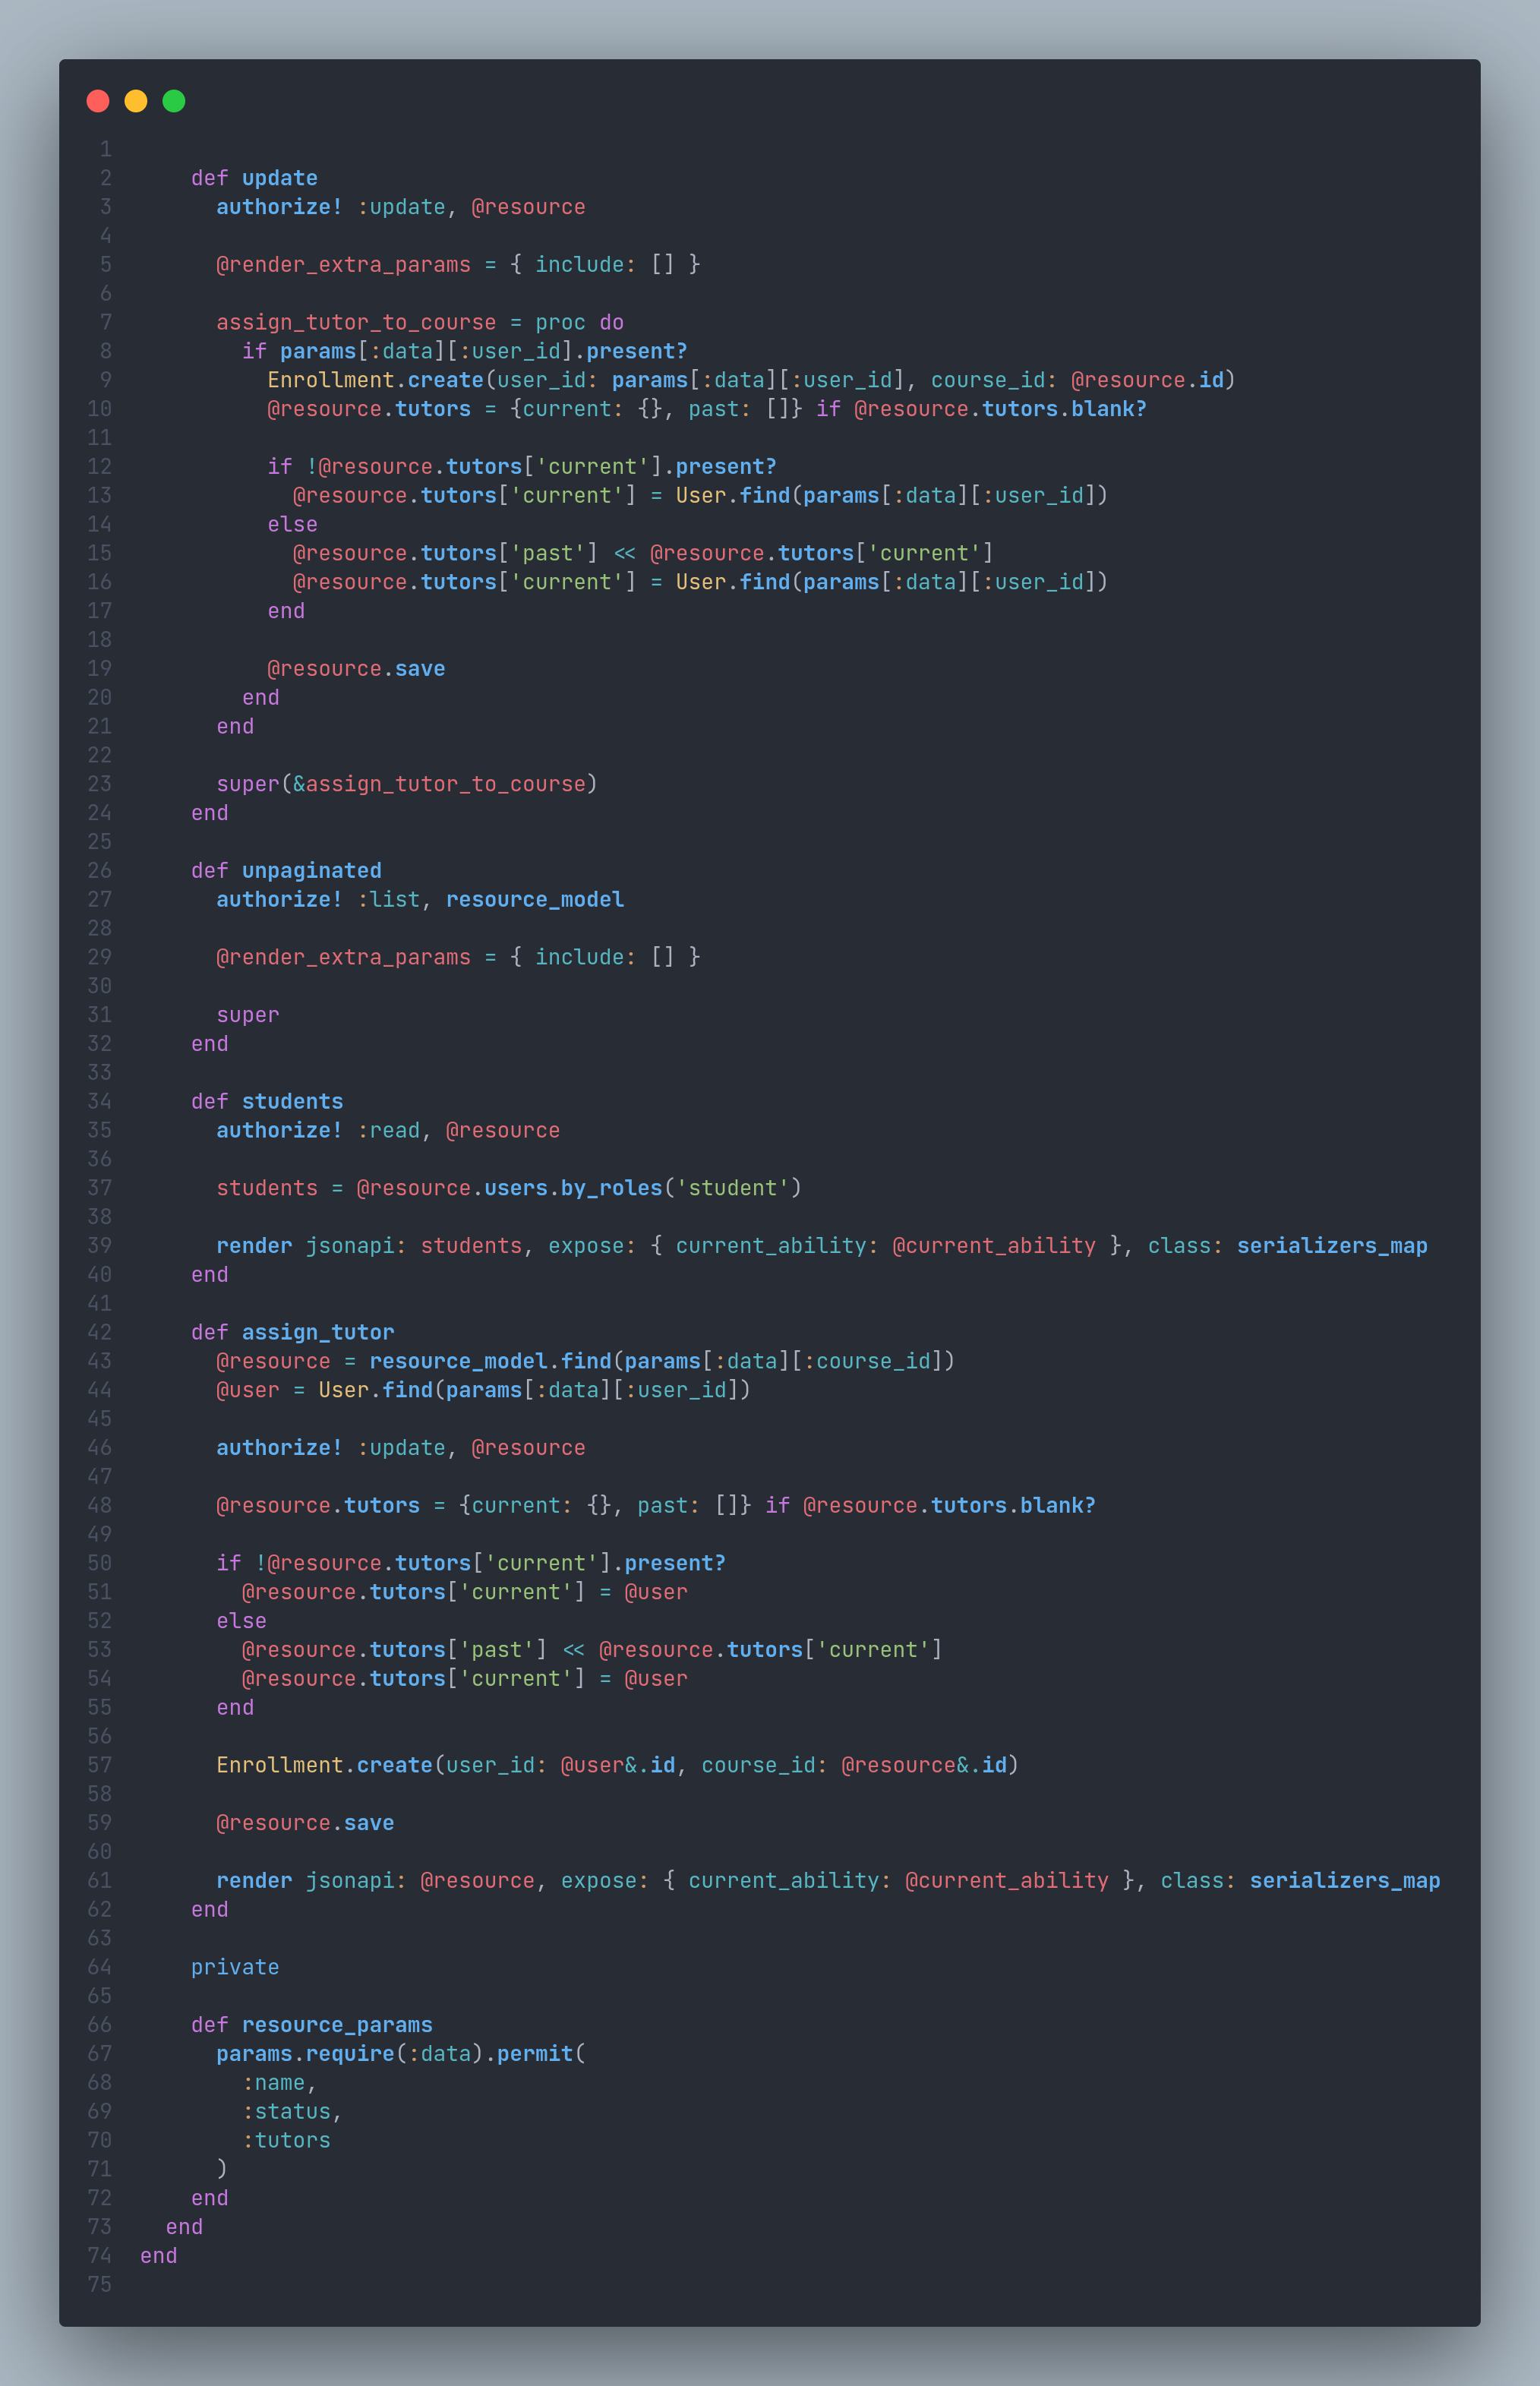
\includegraphics[width=150mm,scale=1]{figures/implementation_and_testing/implementation/backend/courses_controller-2.png}}
        \caption{CoursesController - Part 2}
    \end{figure}


    \noindent\textbf{Serializations}

    \vspace{0.25cm}
    \newendline The STDC web application uses the JSON API specification for serializing the resources. The JSON API specification is a specification for building APIs in JSON. It defines a set of rules for how the resources should be represented in JSON. The JSON API specification is used to ensure that the resources are represented in a consistent way across all the endpoints. 
    In the STDC web application, each model comes with a serializer, that serializer uses the JSONAPI-rails gem to define what should be the out of an endpoint that returns a resource of that model. The JSONAPI-rails gem is a gem that provides a DSL for defining the JSON API specification.

    \vspace{0.25cm}
    \newendline Each serializer inherits from the BaseSerializer, the BaseSerializer is responsible for camelizing all the keys of a serialized resource. This is another way to standarize the responses of each endpiont. The reason for using Camel Case as response is that the client of the STDC uses React JS and the convention in React JS is to use Camel Case for the keys of the JSON objects.

    \vspace{0.25cm}
    \newendline The BaseSerializer is defined as follows:

    \begin{figure}[H]
        \centerline{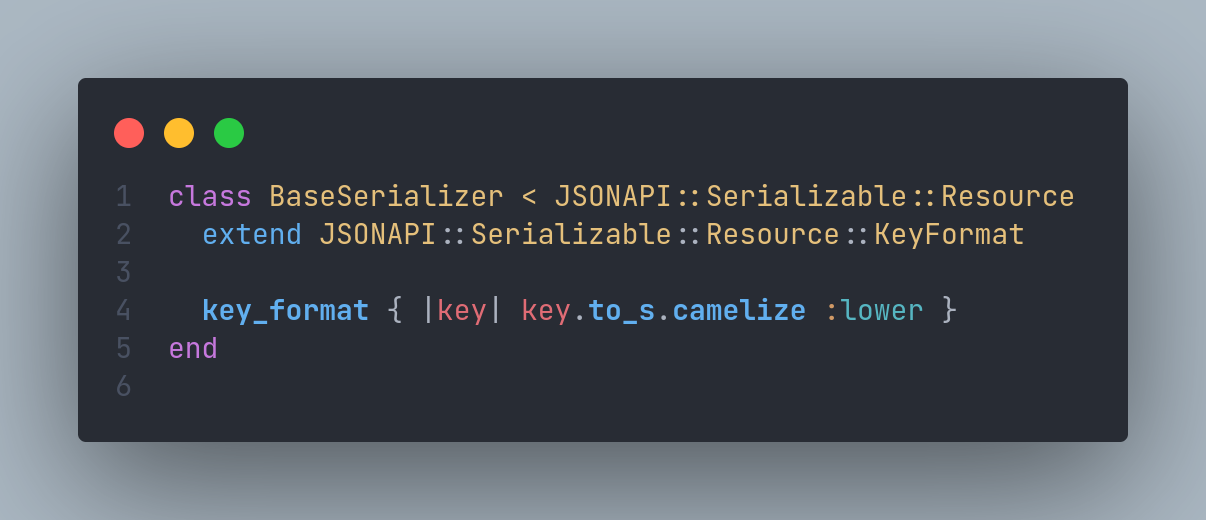
\includegraphics[width=150mm,scale=1]{figures/implementation_and_testing/implementation/backend/base_serializer.png}}
        \caption{BaseSerializer}
    \end{figure}

    \vspace{0.25cm}
    \newendline The SerializersHelper is module that maps all the models to their corresponding serializers. The SerializersHelper is defined as follows:

    \begin{figure}[H]
        \centerline{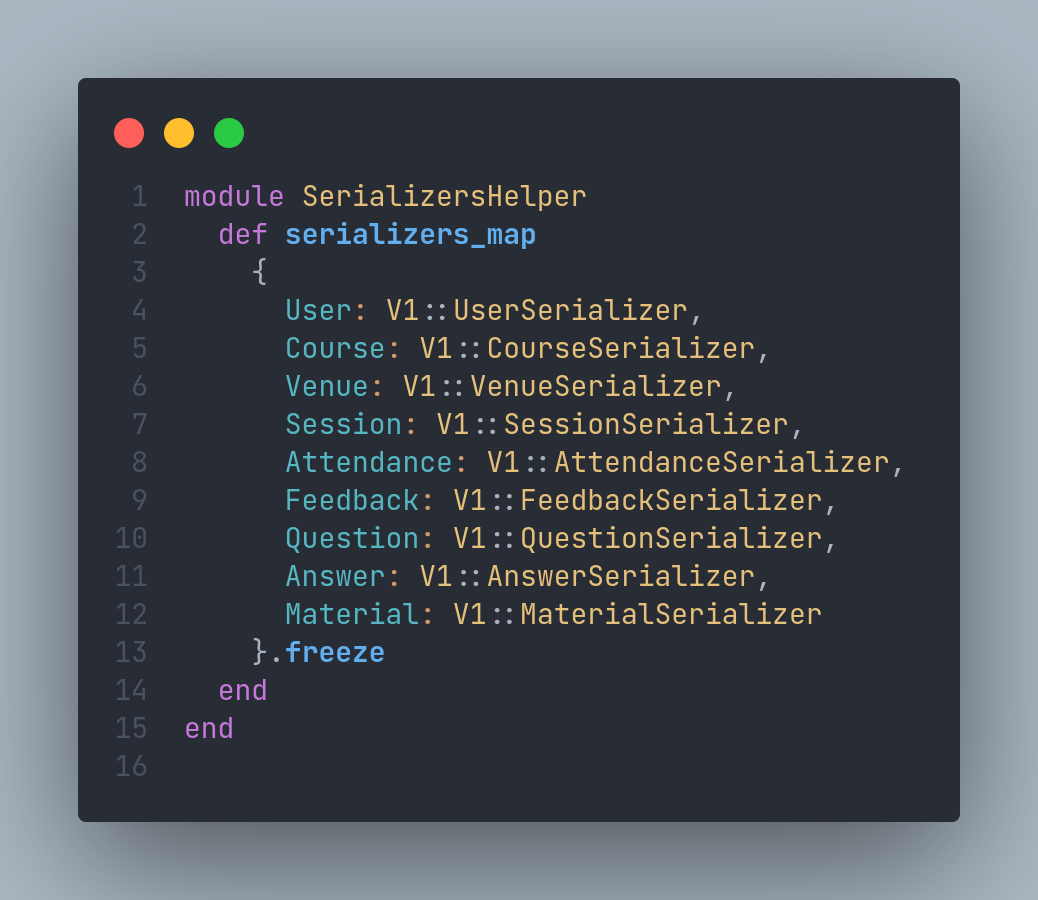
\includegraphics[width=150mm,scale=1]{figures/implementation_and_testing/implementation/backend/serializers_helper.png}}
        \caption{SerializersHelper}
    \end{figure}


    \vspace{0.25cm}
    \newendline The following is an example of a serializer for the Course model:

    \begin{figure}[H]
        \centerline{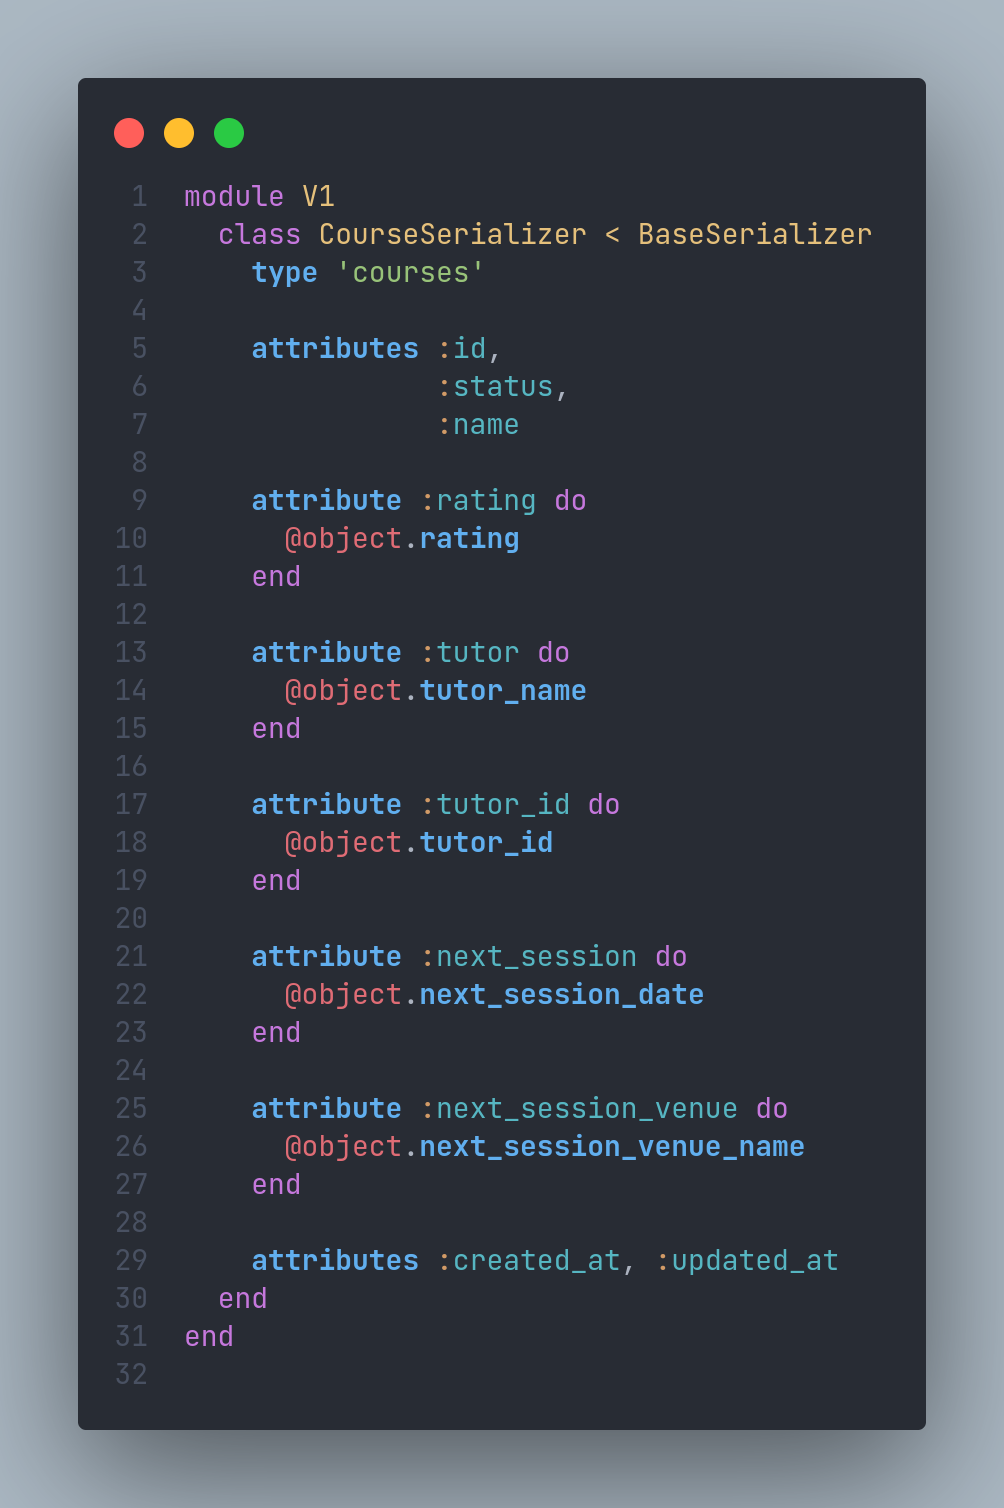
\includegraphics[width=150mm,scale=1]{figures/implementation_and_testing/implementation/backend/courses_serializer.png}}
        \caption{CourseSerializer}
    \end{figure}

    \noindent \textbf{Exception Management}

    \vspace{0.25cm}
    \newendline The STDC web application uses the JSON API specification for serializing the resources this includes the errors. The STDC uses the CustomResponseExceptionSerializer to serialize the errors. The CustomResponseExceptionSerializer is defined as follows:

    \begin{figure}[H]
        \centerline{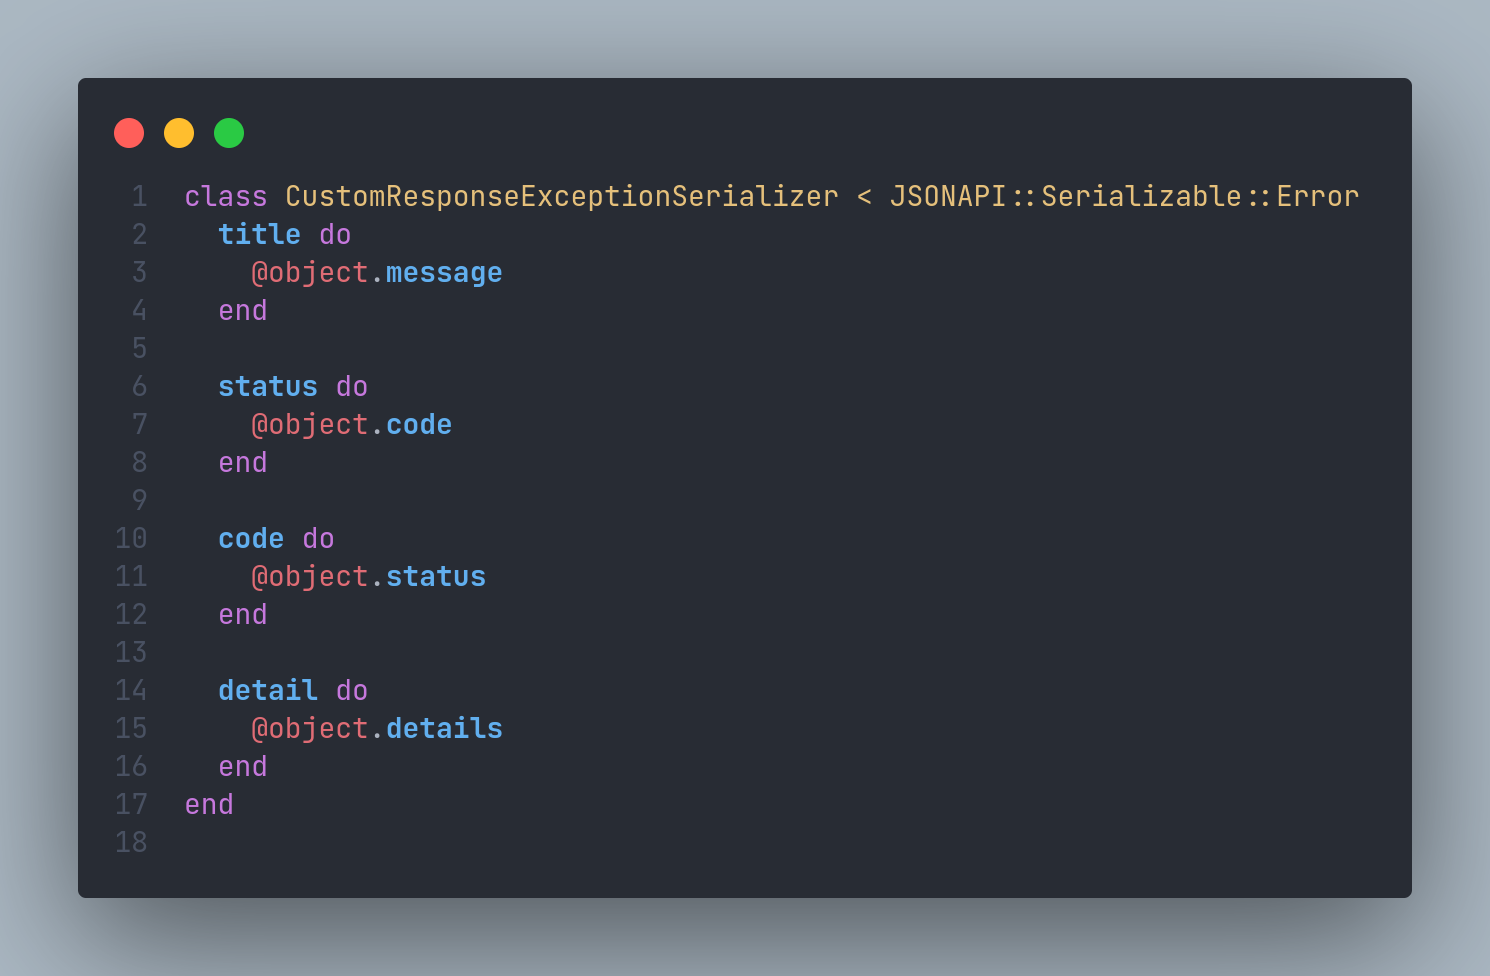
\includegraphics[width=150mm,scale=1]{figures/implementation_and_testing/implementation/backend/custom_response_exception_serializer.png}}
        \caption{CustomResponseExceptionSerializer}
    \end{figure}

    \vspace{0.25cm}
    \newendline The STDC web application uses the ErrorRespondable module to handle the errors that occur in the controllers. The ErrorRespondable module includes standard errors as well as custom errors. 
    The standard errors are the errors that are defined by Rails itself. The custom errors are the errors that are defined in the CustomExceptions module and the JsonErrors. All the errors are handled in the ErrorRespondable in the same way.

    \begin{figure}[H]
        \centerline{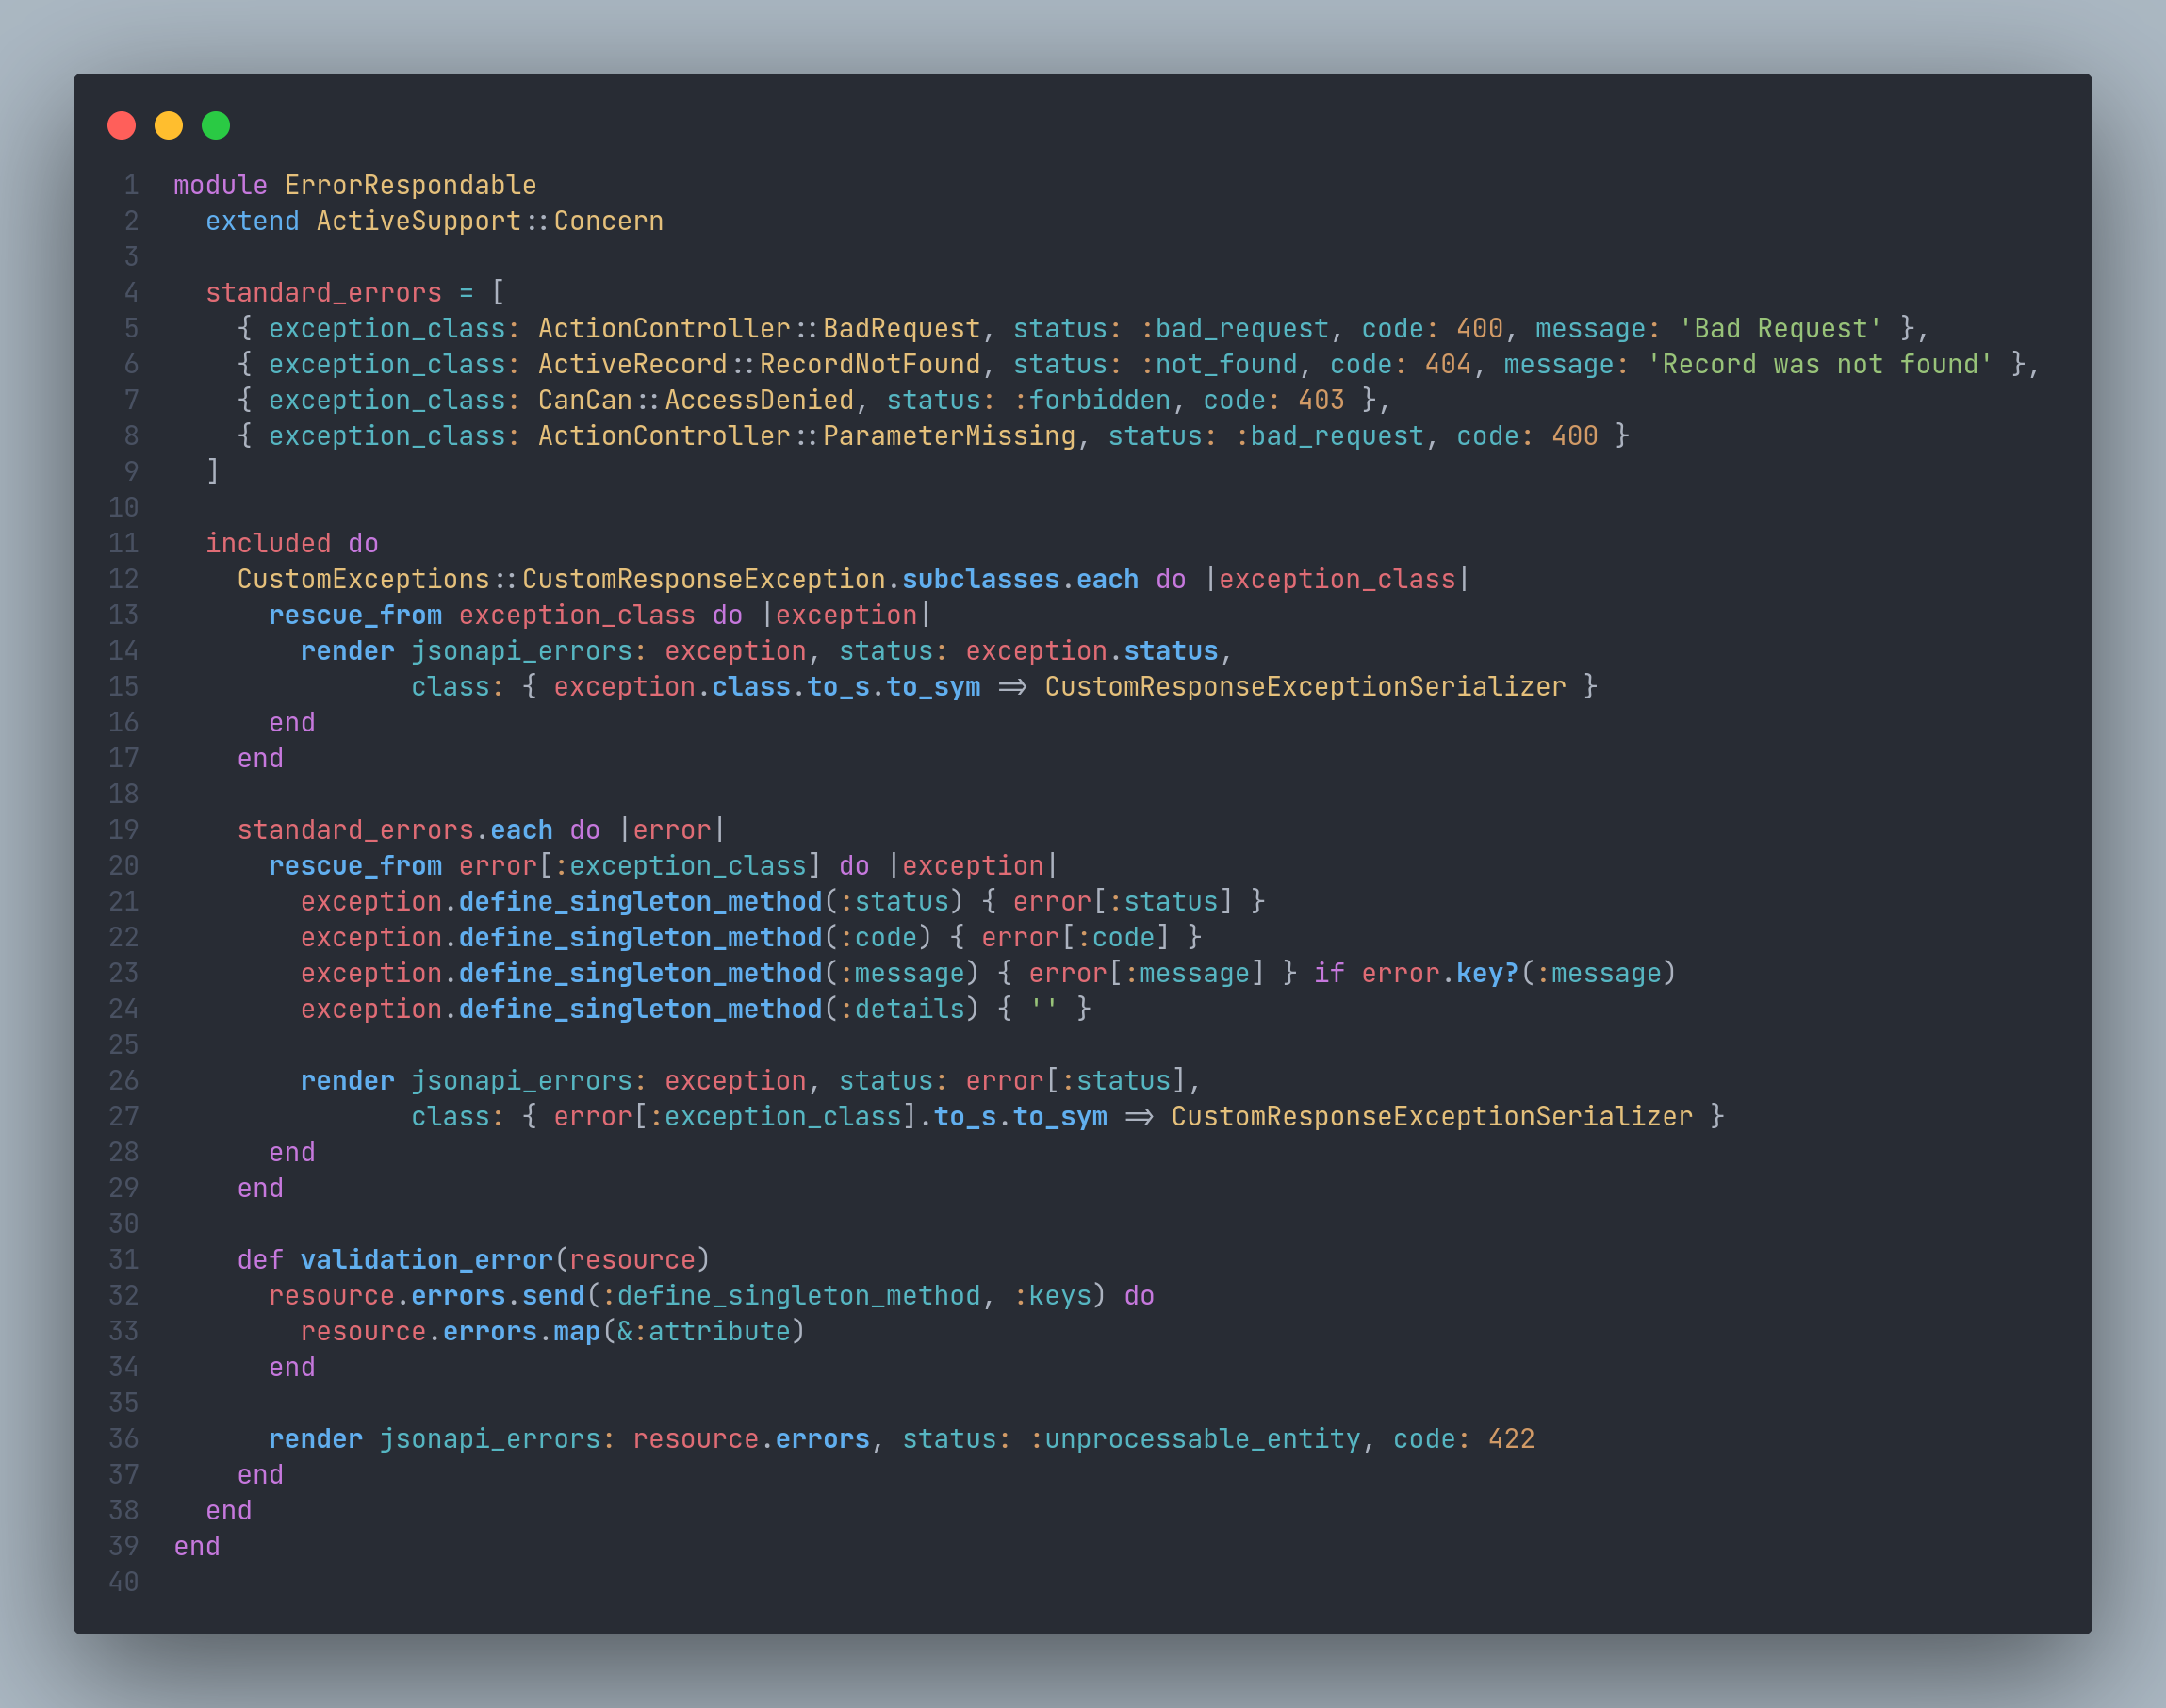
\includegraphics[width=150mm,scale=1]{figures/implementation_and_testing/implementation/backend/error_respondable.png}}
        \caption{ErrorRespondable}
    \end{figure}

    \begin{figure}[H]
        \centerline{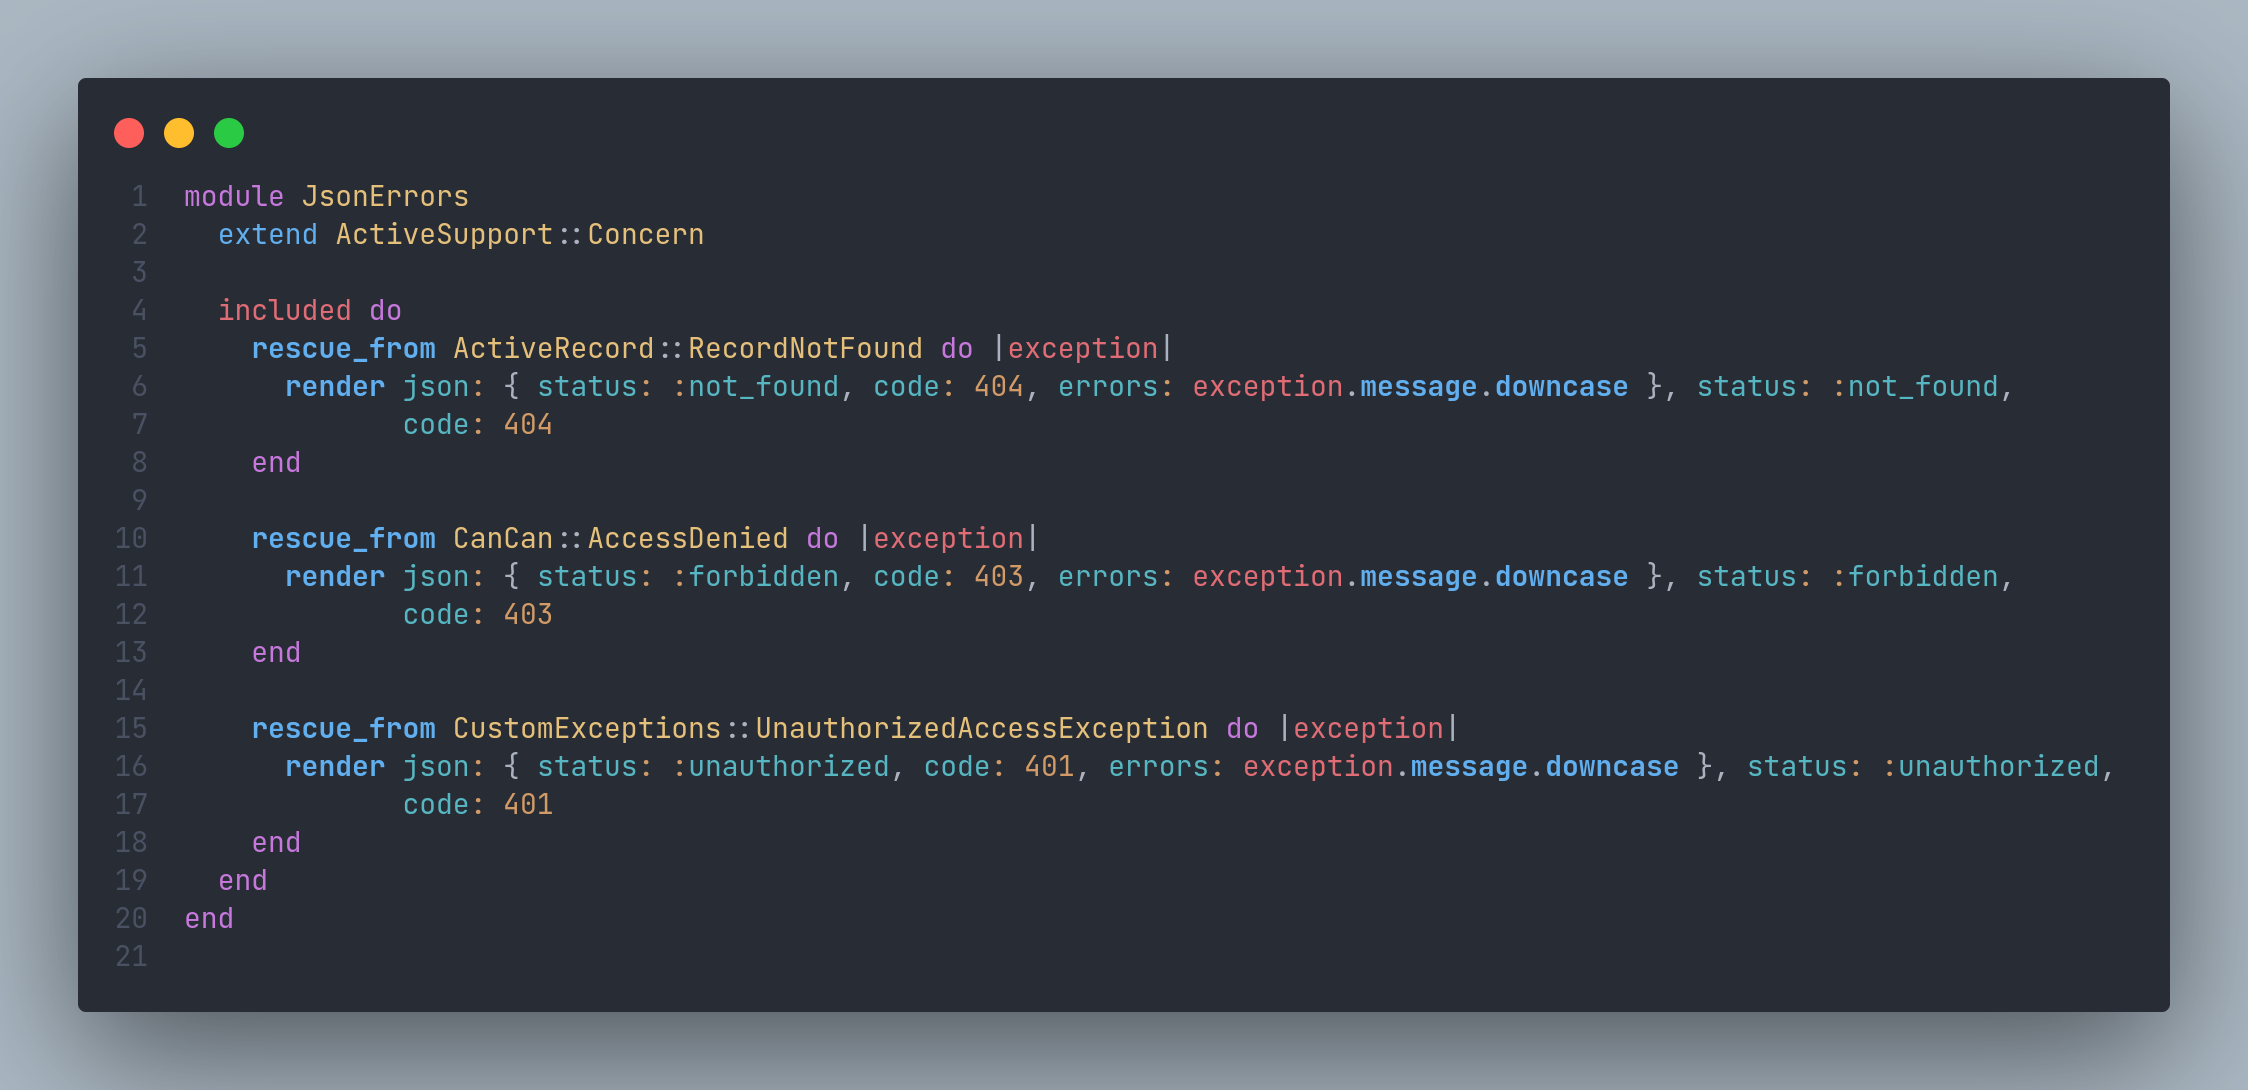
\includegraphics[width=150mm,scale=1]{figures/implementation_and_testing/implementation/backend/json_errors.png}}
        \caption{JsonErrors}
    \end{figure}

    \begin{figure}[H]
        \centerline{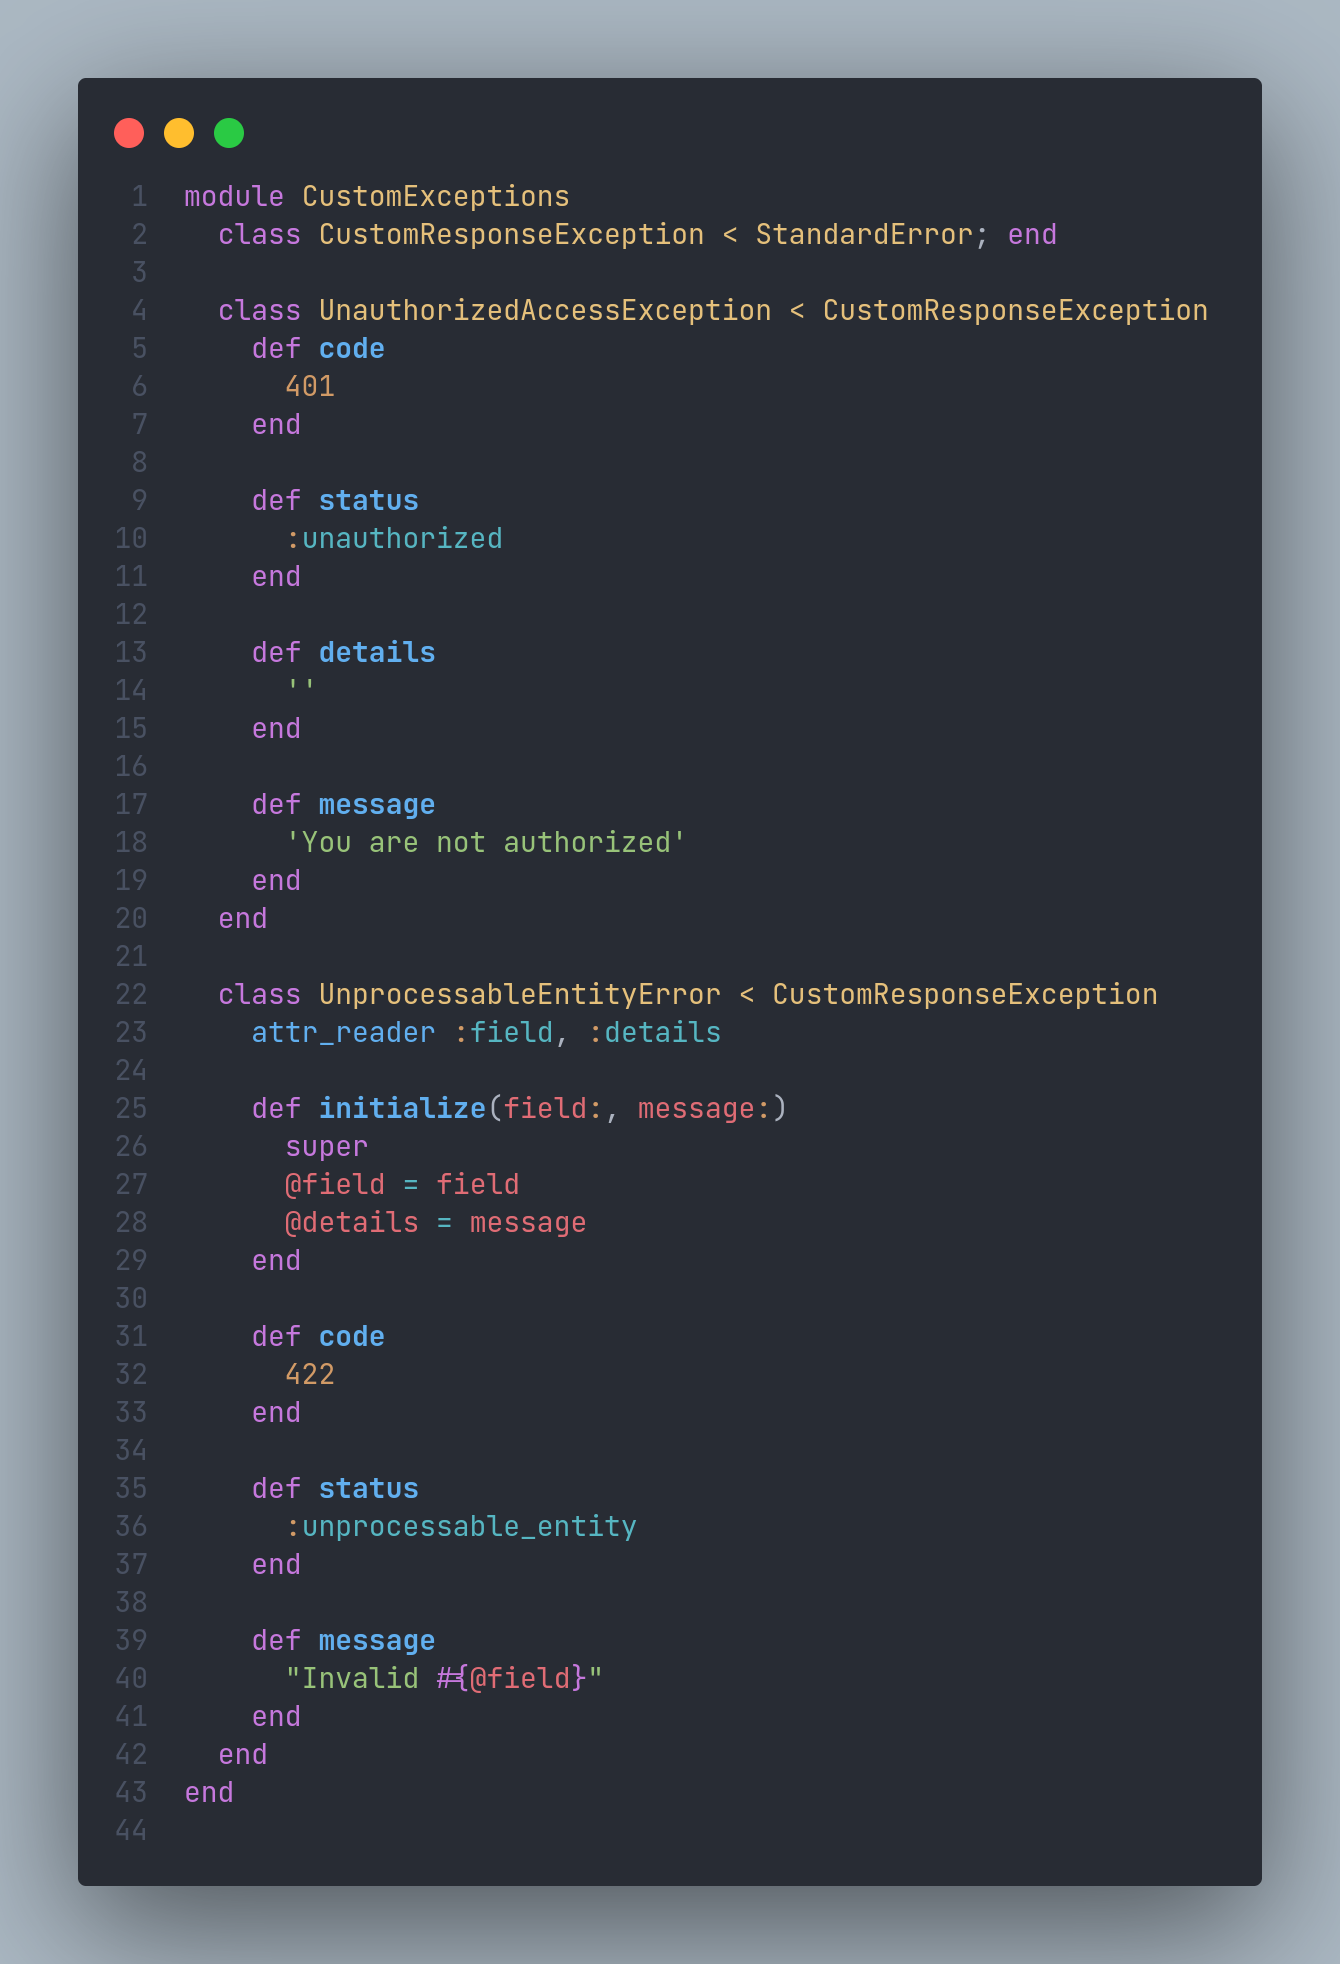
\includegraphics[width=150mm,scale=1]{figures/implementation_and_testing/implementation/backend/custom_exceptions.png}}
        \caption{CustomExceptions}
    \end{figure}

    \vspace{0.25cm}
    \newendline The Common Error Response HTTP Codes are as follows:

    \begin{itemize}
        \item 400: Bad Request (The request was invalid or cannot be served. The exact error is explained in the error payload).
        \item 401: Unauthorized (The request requires an user authentication).
        \item 403: Forbidden (The server understood the request, but is refusing it or the access is not allowed, requires user authorization).
        \item 404: Not Found (There is no resource behind the URI).
        \item 422: Unprocessable Entity (The request was well-formed but was unable to be followed due to semantic errors or invalid payload structure).
        \item 500: Internal Server Error (The server encountered an unexpected condition which prevented it from fulfilling the request).
    \end{itemize}

    \vspace{0.25cm}
    \newendline There are more to the controllers than what has been mentioned in this section, however, the mentioned parts are the most important parts of the controllers. The other parts of the controllers are not mentioned in this section because they are not as important as the mentioned parts and due to the documentation size limitation.\\

    \clearpage

%%%%%%%%%%%%%%%%%%%%%%%%%%%%%%%%%%%%%%%%%%%%%%%%%%%%%%%%%%%%%%%%%%
%%%%%%%%%%%%%%%%%%%%%%%%%%%%%%%%%%%%%%%%%%%%%%%%%%%%%%%%%%%%%%%%%%
%%%%%%%%%%%%%%%%%%%%%%%%%%%%%%%%%%%%%%%%%%%%%%%%%%%%%%%%%%%%%%%%%%
%%%%%%%%%%%%%%%%%%%%%%%%%%%%%%%%%%%%%%%%%%%%%%%%%%%%%%%%%%%%%%%%%%



    \vspace{0.25cm}
    \newendline \textbf{\textit{Results}}\newendline
        The Student Talent Development Center (STDC)'s backend has been implemented using Ruby on Rails. The development of the backend has been done to serve as an API server for the frontend. The backend has also been deployed to Heroku to be used by the frontend, more on this in the coming sections. The backend has no user interface, only API endpoints. However, the backend has API documentations that are generated using Swagger. The following are the API endpoints that are available in the backend of the STDC web application. They are taken from the Swagger API documentations from the deployed backend.

        \begin{figure}[H]
            \begin{minipage}[trim]{1\textwidth}
            \centerline{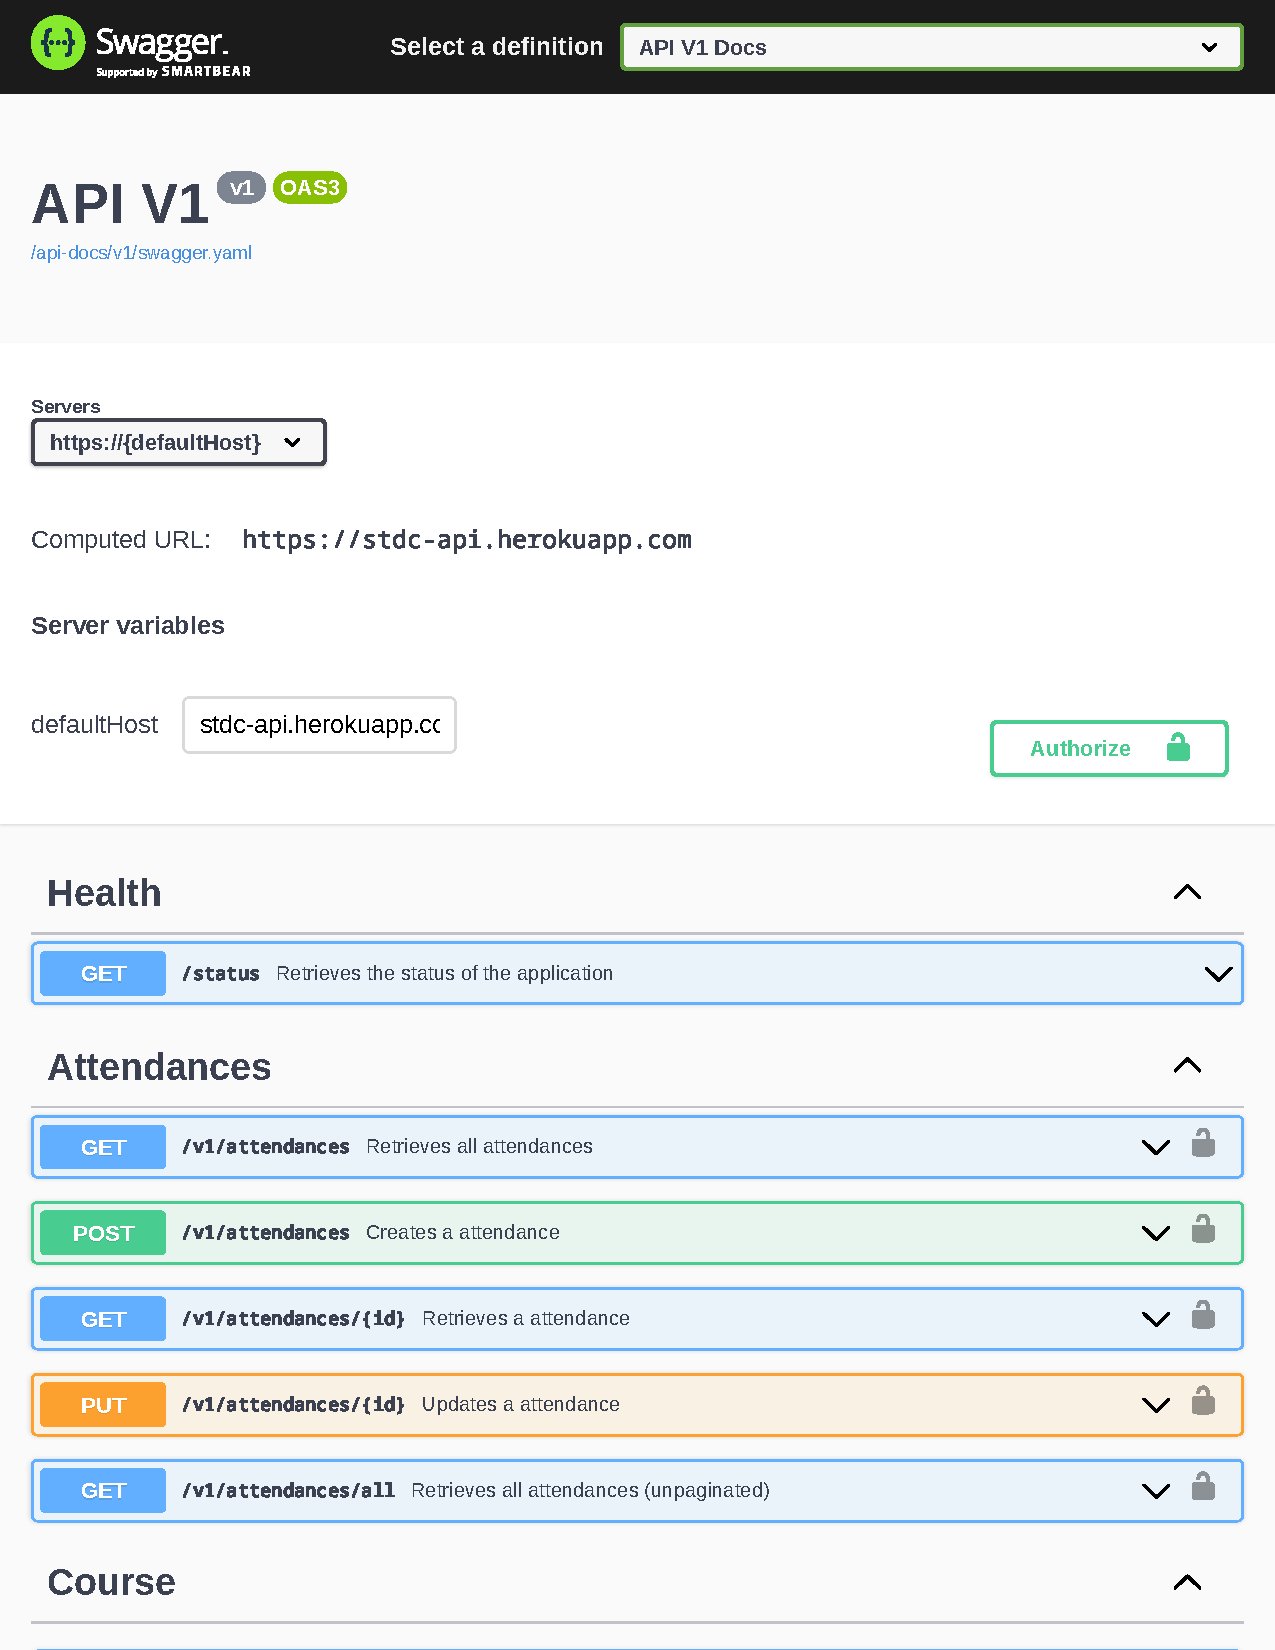
\includegraphics[width=150mm,scale=1]{figures/implementation_and_testing/implementation/backend/swagger-1.pdf}}
            \caption{Swagger - Part 1}
            \end{minipage}
        \end{figure}

        \begin{figure}[H]
            \begin{minipage}[trim]{1\textwidth}
            \centerline{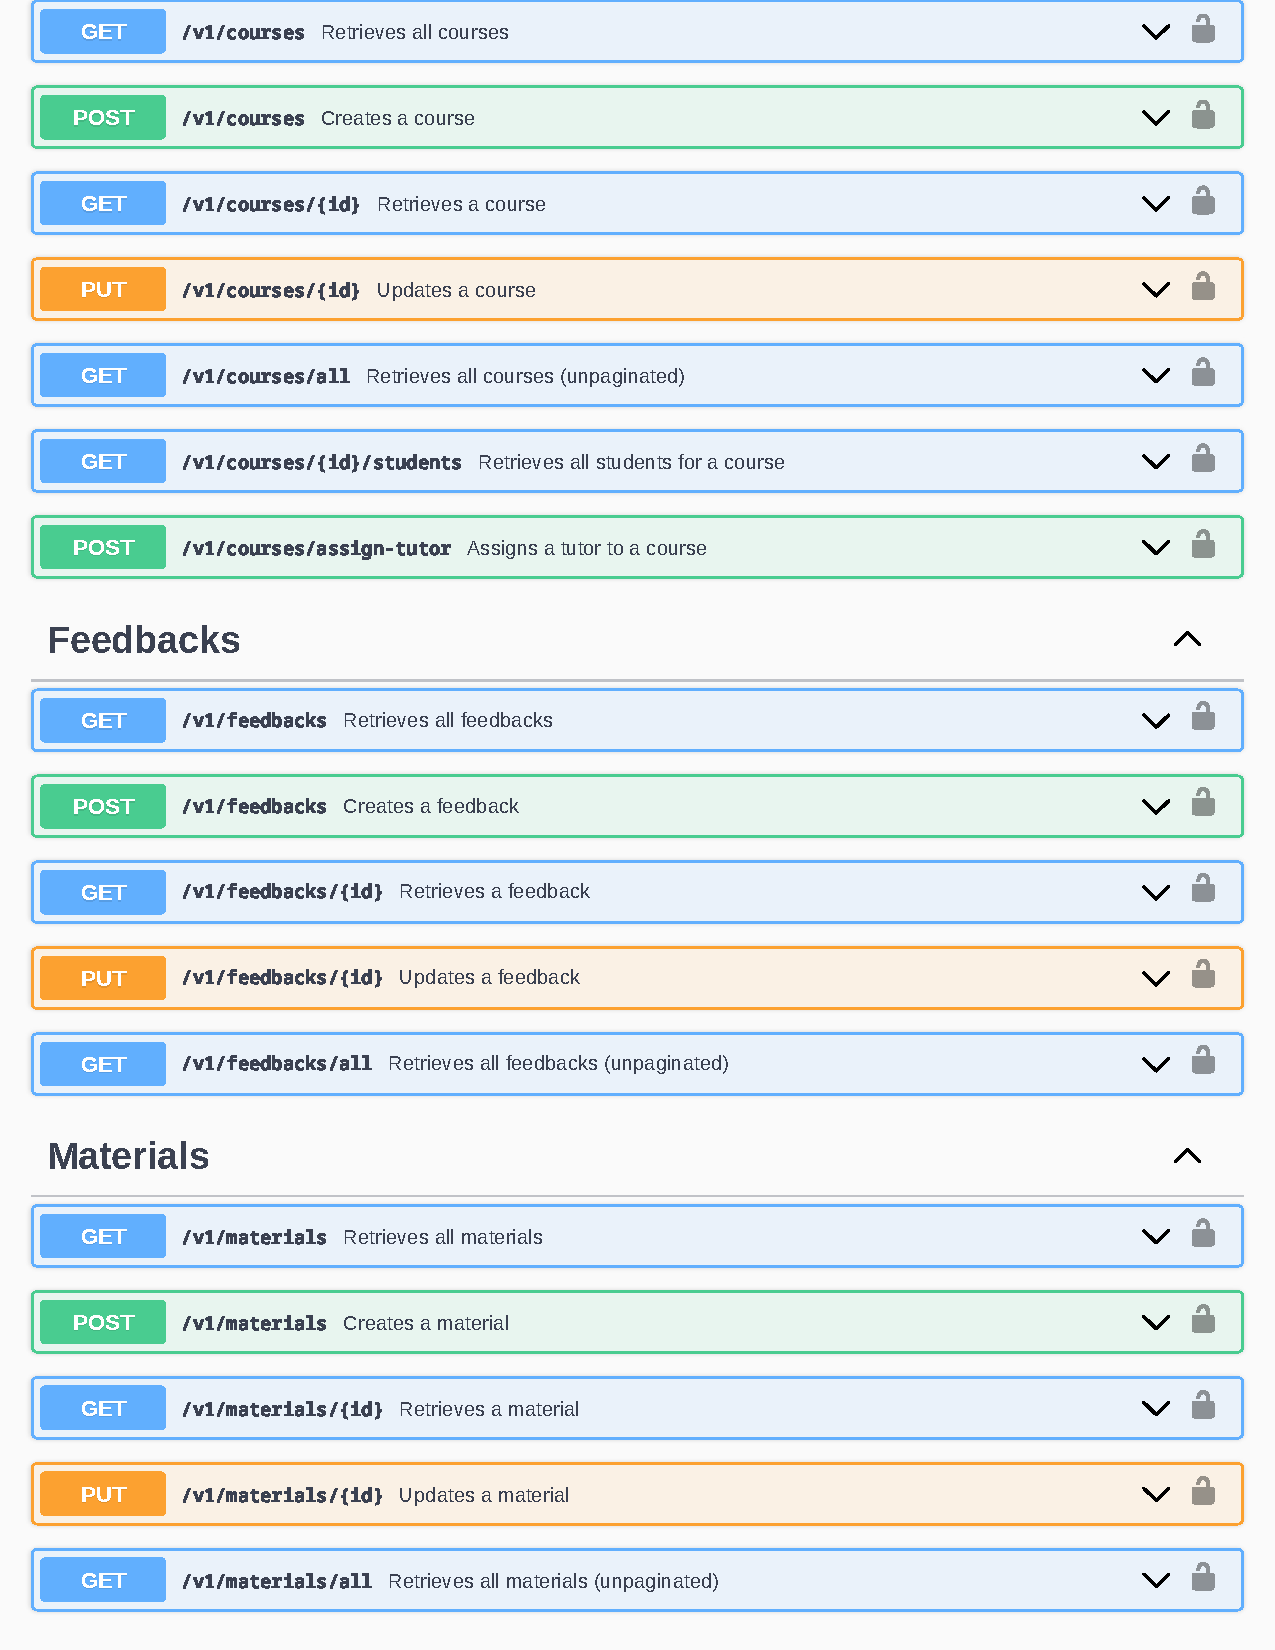
\includegraphics[width=150mm,scale=1]{figures/implementation_and_testing/implementation/backend/swagger-2.pdf}}
            \caption{Swagger - Part 2}
            \end{minipage}
        \end{figure}


        \begin{figure}[H]
            \begin{minipage}[trim]{1\textwidth}
            \centerline{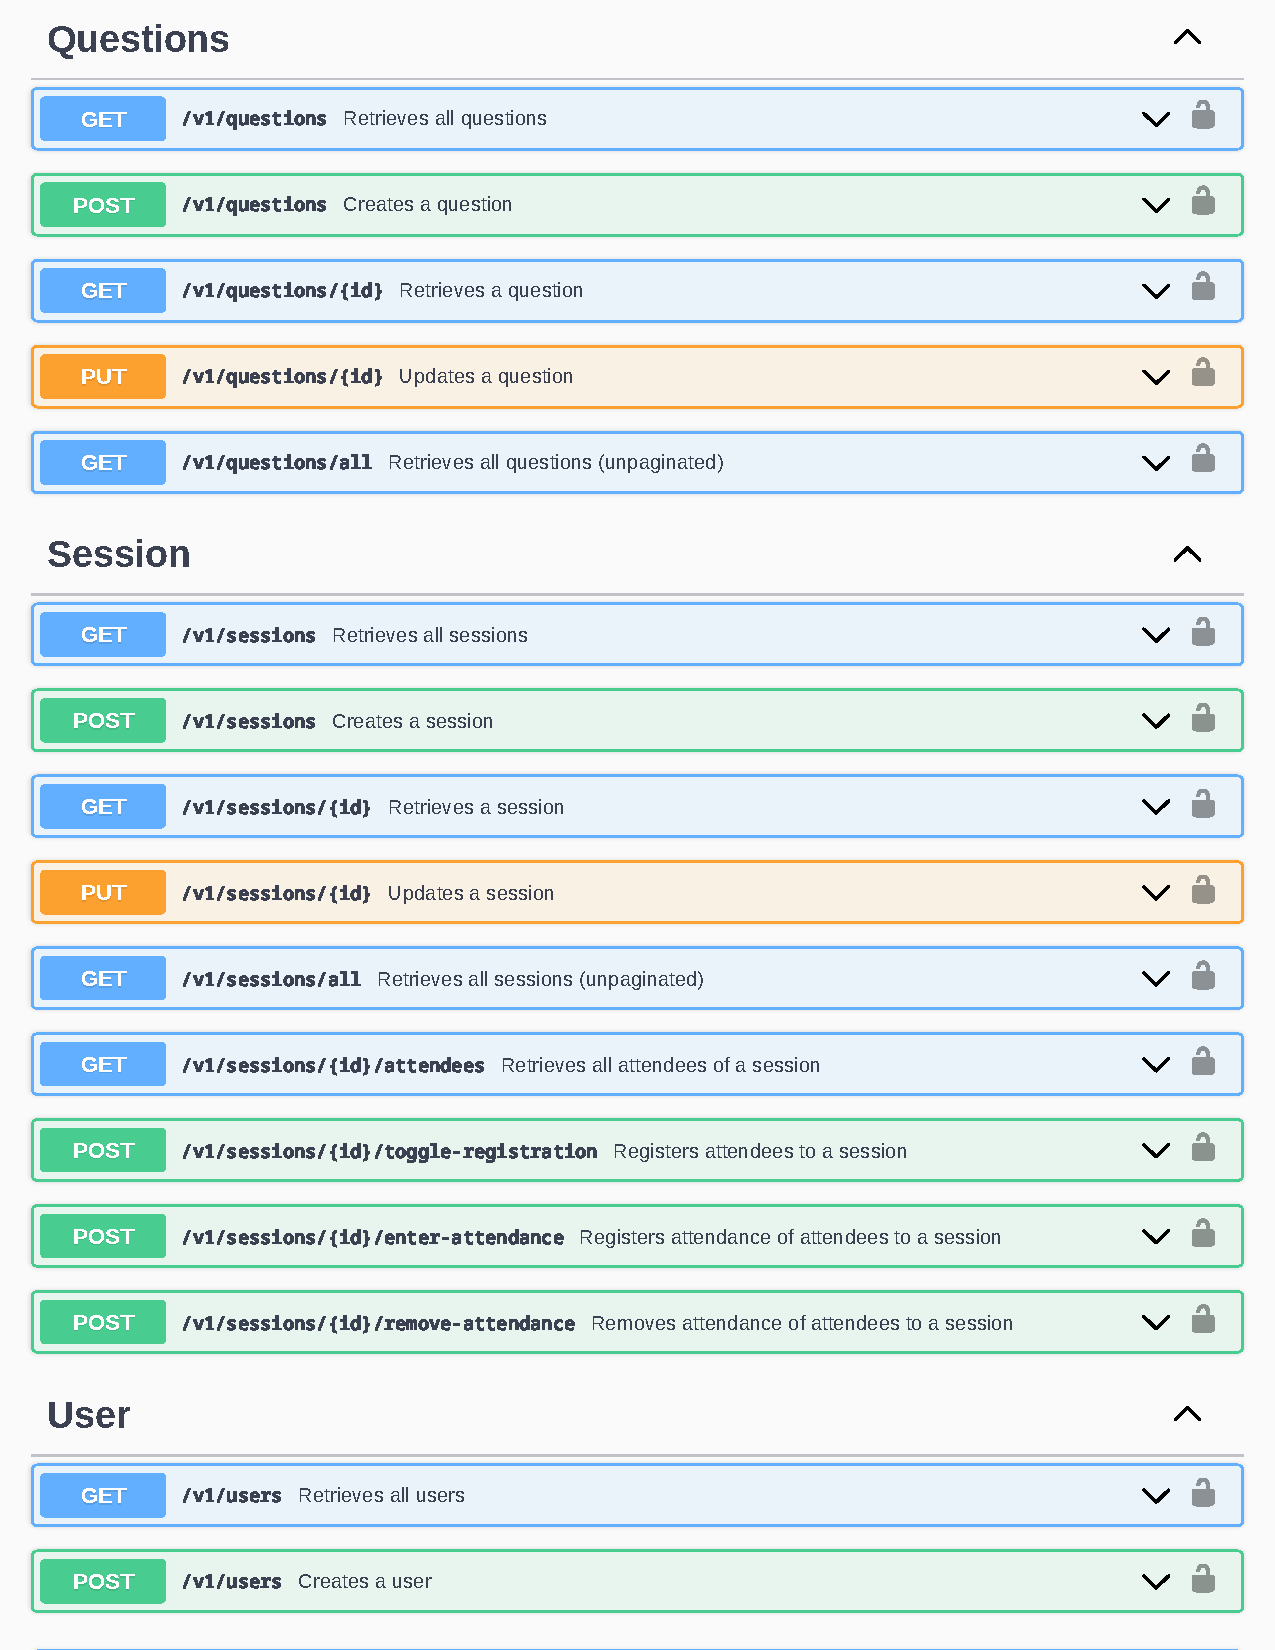
\includegraphics[width=150mm,scale=1]{figures/implementation_and_testing/implementation/backend/swagger-3.pdf}}
            \caption{Swagger - Part 3}
            \end{minipage}
        \end{figure}


        \begin{figure}[H]
            \begin{minipage}[trim]{1\textwidth}
            \centerline{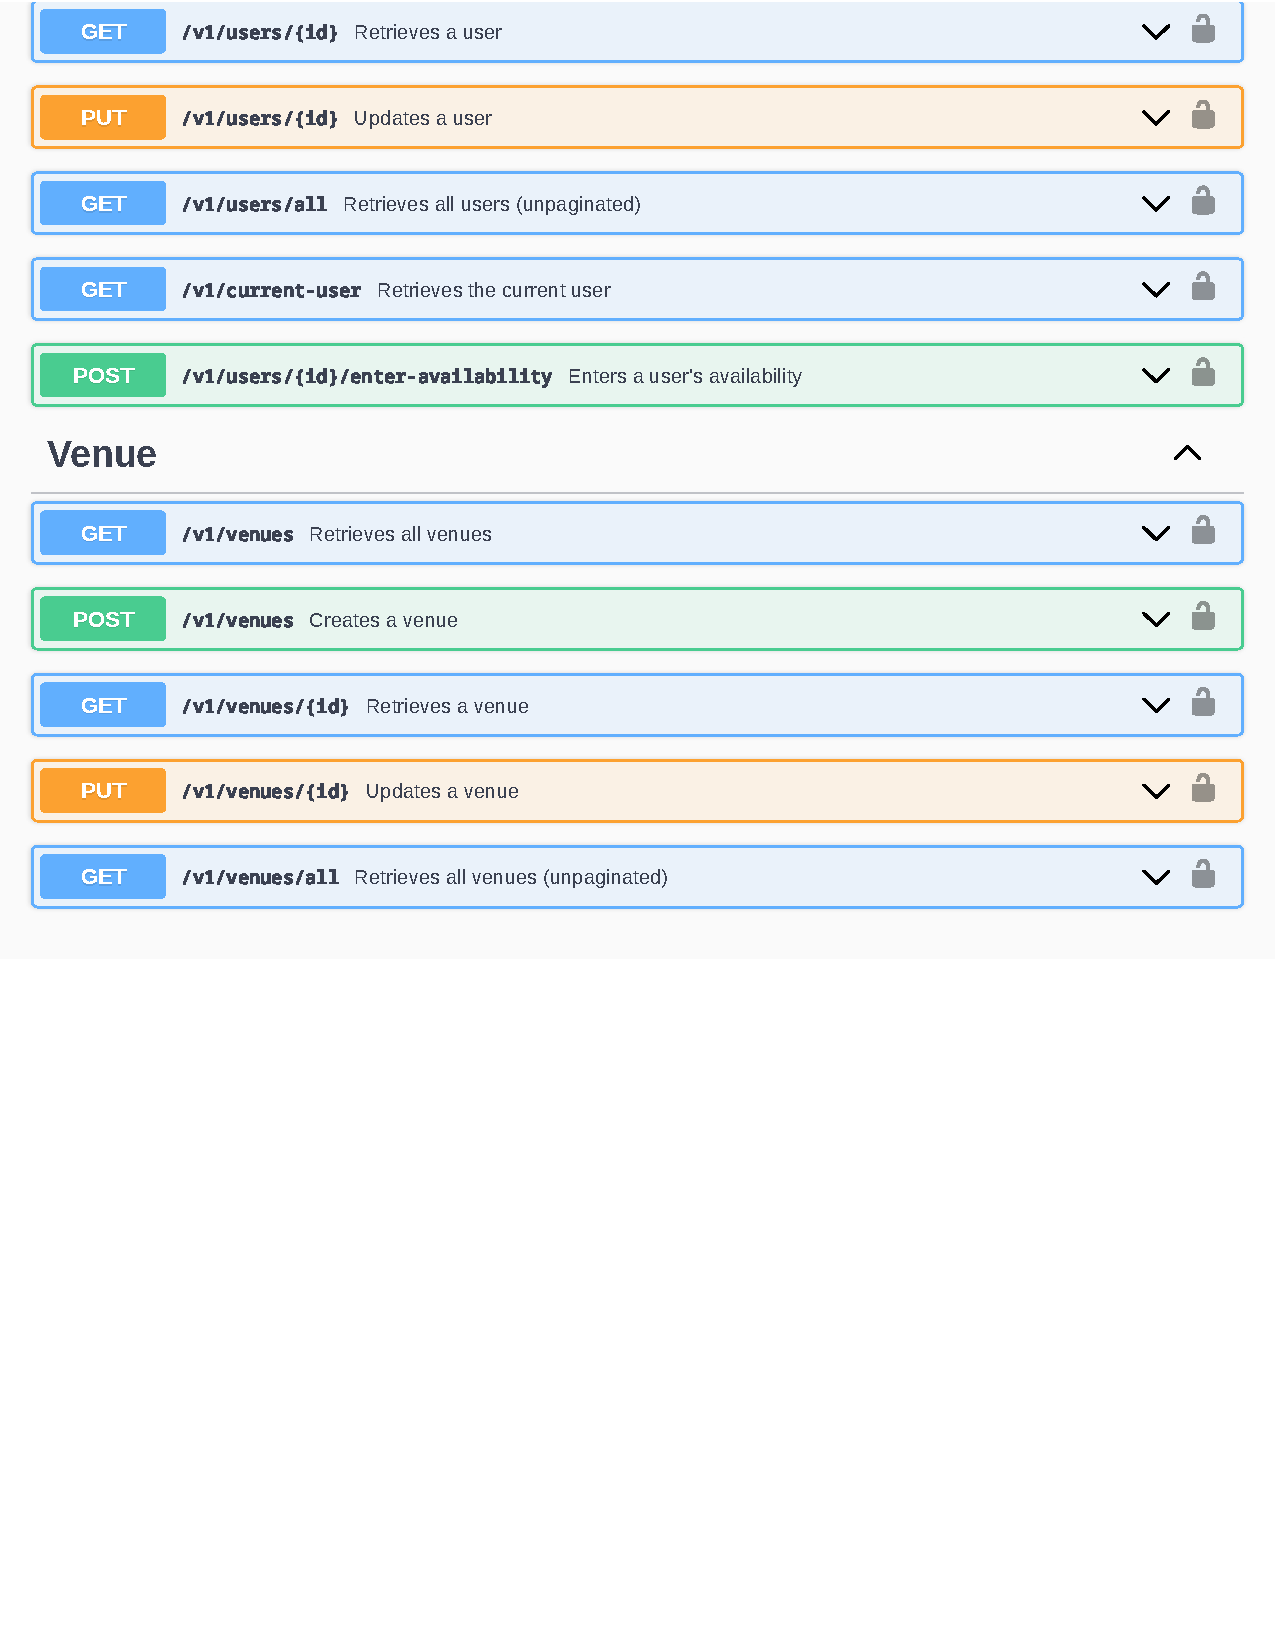
\includegraphics[width=150mm,scale=1]{figures/implementation_and_testing/implementation/backend/swagger-4.pdf}}
            \caption{Swagger - Part 4}
            \end{minipage}
        \end{figure}
        
        \begin{figure}[H]
            \centerline{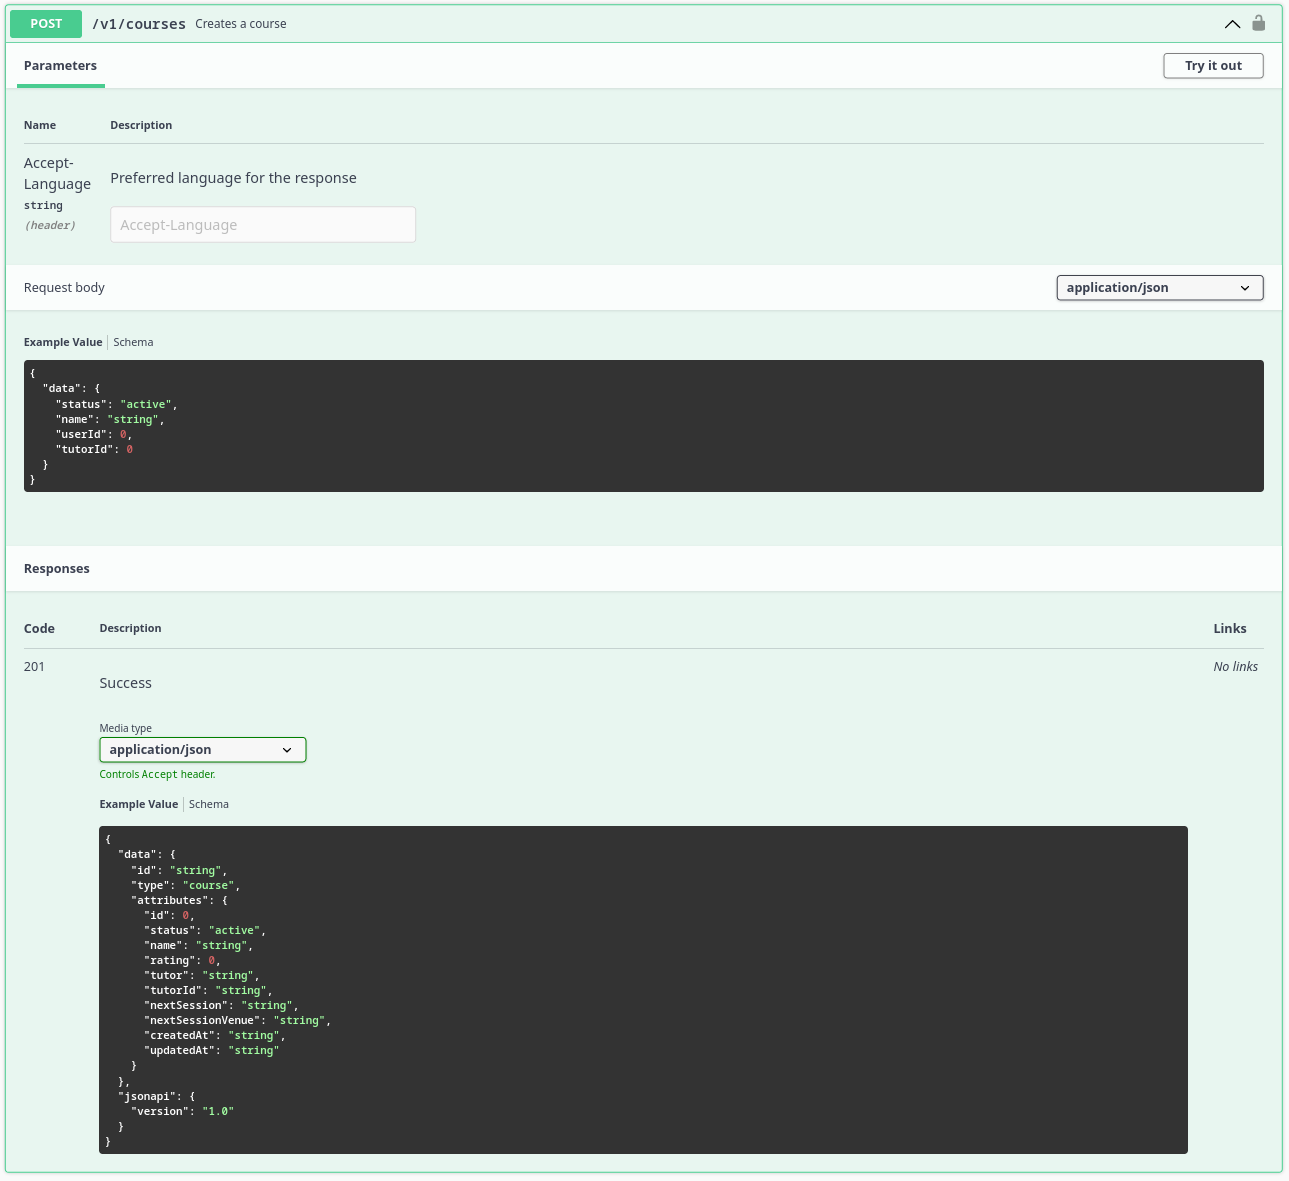
\includegraphics[width=150mm,scale=1]{figures/implementation_and_testing/implementation/backend/response request.png}}
            \caption{Swagger - Course Post's Request and Response}
        \end{figure}
        
    \clearpage

    %%%%%%%%%%%%%%%%%%%%%%%%%%%%%%%%%%%%%%%%%%%%%%%%%%%%%%%%%%%%%%%%%%
    %%%%%%%%%%%%%%%%%%%%%%%%%%%%%%%%%%%%%%%%%%%%%%%%%%%%%%%%%%%%%%%%%%
    %%%%%%%%%%%%%%%%%%%%%%%%%%%%%%%%%%%%%%%%%%%%%%%%%%%%%%%%%%%%%%%%%%
    %%%%%%%%%%%%%%%%%%%%%%%%%%%%%%%%%%%%%%%%%%%%%%%%%%%%%%%%%%%%%%%%%%
    

    \vspace{0.25cm}
    \newendline \textbf{\textit{Summary}}\newendline
        In addition to the discussed aspects, there are several areas in the backend of the STDC web application that can be improved to achieve optimal performance. However, due to time constraints, only a limited number of improvements have been implemented. Some of the areas that require attention include resolving the tutor's association with a session and a course, addressing potential errors and suboptimal coding practices, and enhancing code quality.

        \vspace{0.25cm}
        \newendline Considering the context of the project, it is worth exploring the concept of microservices for the STDC application. As the university is relatively large, implementing a microservice architecture could offer significant advantages. This approach involves breaking down the application into separate services, such as user management and notifications. Each department could have its own system, integrated with others, resulting in a more scalable and modular application architecture.
        
        \vspace{0.25cm}
        \newendline Furthermore, it is important to acknowledge that while the backend meets the functional requirements, the code quality can be further improved. Given the time constraints and limitations, the current implementation has been a commendable effort. However, to ensure long-term maintainability and scalability, it is necessary to address code clean-ups and implement various improvements.
        
        \vspace{0.25cm}
        \newendline In conclusion, the backend implementation of the STDC web application using Ruby on Rails has provided a solid foundation for the overall functionality of the system. The deployment on Heroku ensures accessibility, and the provision of API endpoints facilitates seamless communication with the frontend. While only the important aspects have been covered in this section, there are numerous other considerations and enhancements required for a comprehensive and refined application.
        
        \vspace{0.25cm}
        \newendline To achieve the optimal state, future work should focus on resolving the tutor association, improving code quality, and exploring microservice architecture possibilities. With further development and refinement, the backend of the STDC web application can deliver an even more robust and efficient user experience.
    \clearpage

    
\end{justify}
\clearpage


% ===============================================================================================
% ===============================================================================================
% ===============================================================================================
% ===============================================================================================


\subsection{Frontend Implementation (Client)}
\begin{justify}
     The following section shows how the implementation for the Client (the frontend) has been done for the Student Talent Development Center Web Application.\\

    \vspace{0.25cm}
    \newendline \textbf{\textit{Technologies Used}}\newendline
        The frontend of the application for the Student Talent Development Center (STDC) makes use of a variety of technologies in order to create a user interface that is both straightforward and interesting to interact with.

        \vspace{0.25cm}
        \newendline The frontend is built on top of a library written in JavaScript called React, which is used extensively. React is a framework that enables the rapid development of user interfaces for single-page or mobile applications. It was created and is maintained by Facebook in collaboration with a community of developers.
        
        \vspace{0.25cm}
        \newendline Auth0 is an authentication and authorization platform that makes user authentication more straightforward by supplying a solution that is friendly to developers. The application can effortlessly manage authentication procedures for its users as a result of its integration of Auth0. Auth0 has also been used in the backend as previously mentioned.
        
        \vspace{0.25cm}
        \newendline For React applications, React Query fills the role of the library that was previously lacking for fetching data. It simplifies the process of retrieving data from the server, as well as caching, synchronizing, and updating that data, which in turn improves the application's performance and efficiency.
        
        \vspace{0.25cm}
        \newendline Declarative composition is made possible within the application by utilizing the React Router, which is a collection of navigational components. It doesn't matter whether you're using it to generate bookmarkable URLs for web apps or to make navigation easier in React Native; React Router integrates with React in a seamless manner.
        
        \vspace{0.25cm}
        \newendline The use of React Hook Form allows for efficient management of the data collected from forms. This lightweight library, which does not depend on any external dependencies, simplifies form data management. As a result, complexity is reduced, and development efficiency is increased.
        
        \vspace{0.25cm}
        \newendline A simple and straightforward approach to incorporating notifications into the application is provided by the React Toastify library. It provides a user-friendly option for displaying important messages to the users of the system.
        
        \vspace{0.25cm}
        \newendline Google's Material Design was adapted into an implementation called Material UI, which is a comprehensive collection of React components. The frontend of the STDC application adheres to established design principles and ensures a visually appealing and consistent user interface by utilizing Material UI. These goals were accomplished successfully.
        
        \vspace{0.25cm}
        \newendline A well-known promise-based HTTP client called Axios makes it simple to exchange information between the frontend and the backend of a website. It provides a user-friendly application programming interface (API) for submitting HTTP requests in both the browser and Node.js environments, in our case, React JS.
        
        \vspace{0.25cm}
        \newendline Redux, which is a container that provides a predictable state, is an essential component in the process of managing the application's state. It makes it possible to have consistent behavior across a variety of environments, such as the client, the server, and native platforms, while also improving the testability of the system.
        
        \vspace{0.25cm}
        \newendline A specialized library called the mui-rhf-library has been developed to integrate Material UI and React Hook Form. It makes the process of integration easier and ensures that there will be no hiccups in the interaction between the two libraries.
        
        \vspace{0.25cm}
        \newendline When it comes to describing, producing, consuming, and visually representing RESTful web services, OpenAPI, which is a specification for machine-readable interface files, is an extremely important component. It is put to use to generate services that are based on the API, which promotes the efficient and standardized development of software.
        
        \vspace{0.25cm}
        \newendline Yup is a JavaScript schema builder that makes it possible to validate and parse data values. It provides a reliable solution for validating the data within the application, helping to guarantee the accuracy of the data as well as its integrity.
        
        \vspace{0.25cm}
        \newendline Because it uses a combination of these frontend technologies, the STDC application is able to provide users with an experience that is seamless, interactive, and visually appealing. Additionally, the application is able to manage data fetching, form handling, authentication, and state management in an efficient manner.
    \clearpage


%%%%%%%%%%%%%%%%%%%%%%%%%%%%%%%%%%%%%%%%%%%%%%%%%%%%%%%%%%%%%%%%%%
%%%%%%%%%%%%%%%%%%%%%%%%%%%%%%%%%%%%%%%%%%%%%%%%%%%%%%%%%%%%%%%%%%
%%%%%%%%%%%%%%%%%%%%%%%%%%%%%%%%%%%%%%%%%%%%%%%%%%%%%%%%%%%%%%%%%%
%%%%%%%%%%%%%%%%%%%%%%%%%%%%%%%%%%%%%%%%%%%%%%%%%%%%%%%%%%%%%%%%%%



    \vspace{0.25cm}
    \newendline \textbf{\textit{Authentication}}\newendline
        Auth0 allows you to add authentication to your React application quickly and to gain access to user profile information. It also enables you to use a variety of authentication methods, including social media, username and password, and multi-factor authentication. The authentication process is handled entirely by Auth0, which means that you do not have to worry about implementing authentication protocols. The backend of the STDC application has been configured to use Auth0 for authentication purposes. Now, let's take a look at how the Auth0 has been integrated into the frontend of the STDC application.
    
        \vspace{0.25cm}
        \newendline First of all, in order to use Auth0 in the frontend, you need to install the Auth0 React SDK. The Auth0 React SDK is a library that allows you to integrate Auth0 into your React application. The Auth0 integration also requires an Auth0 application to be made. The process of how to create an Auth0 application is not mentioned here since it is out of the scope of this section. Nevertheless some of the configuration that need to be done in the process are crucial to mention here.

        \begin{itemize}
            \item Application Keys: In order to communicate with Auth0, the frontend needs to have the application keys. The application keys are the client ID and the client secret. The client ID and the client secret are used to identify the application to Auth0. The client ID and the client secret are used to generate the access token and the refresh token. The access token and the refresh token are used to authenticate the user.

            \begin{figure}[H]
                \centerline{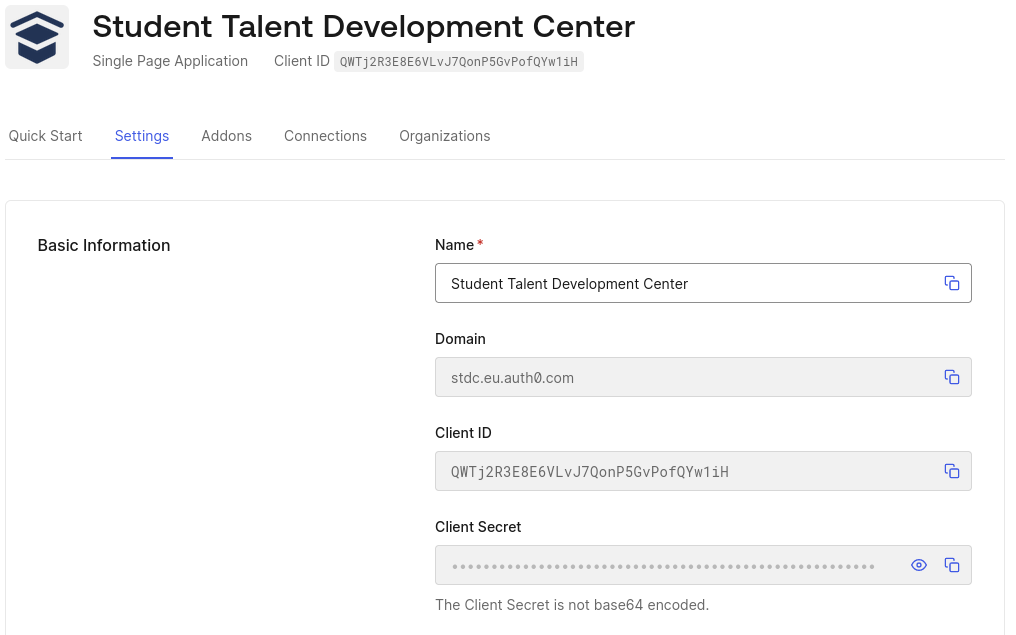
\includegraphics[width=150mm,scale=1]{figures/implementation_and_testing/implementation/frontend/ApplicationKeys.png}}
                \caption{Auth0 Dashboard - Application Keys}
            \end{figure}
        
            
            \item Allowed Callback URLs: The allowed callback URLs are the URLs that Auth0 will redirect the user to after the user has been authenticated. The allowed callback URLs are used to redirect the user to the frontend after the user has been authenticated. It is configured in the Auth0 application using the Auth0 dashboard.
            \item Allowed Logout URLs: The allowed logout URLs are the URLs that Auth0 will redirect the user to after the user has been logged out. The allowed logout URLs are used to redirect the user to the frontend after the user has been logged out. It is configured in the Auth0 application using the Auth0 dashboard.
            \item Allowed Web Origins: The allowed web origins are the URLs that Auth0 will use to silently authenticate the user. The allowed web origins are used to silently authenticate the user. It is configured in the Auth0 application using the Auth0 dashboard.

            \begin{figure}[H]
                \centerline{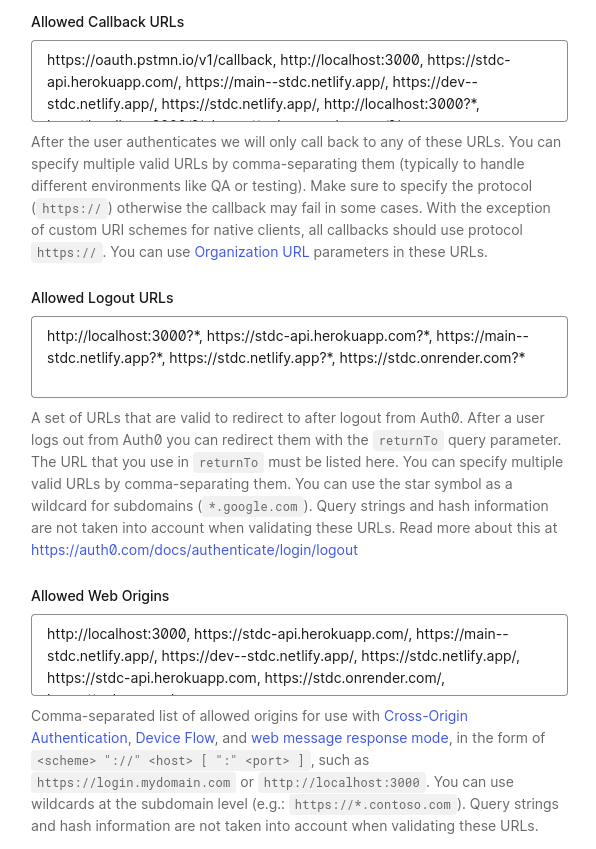
\includegraphics[width=150mm,scale=1]{figures/implementation_and_testing/implementation/frontend/URLS.png}}
                \caption{Auth0 Dashboard - Allowed URLs}
            \end{figure}
        \end{itemize}


        \vspace{-0.25cm}
        \newendline In order to use Auth0, the Auth0Provider component needs to be wrapped around the application. The Auth0Provider component is responsible for initializing the Auth0 SDK and providing the Auth0 SDK to the application. The Auth0Provider component is defined as follows:
        
        \vspace{0.25cm}
        \newendline The Auth0Provider component is wrapped around the application in the index.js file. The index.js file is the entry point of the application. The index.js file is as follows:
        
        \begin{figure}[H]
            \centerline{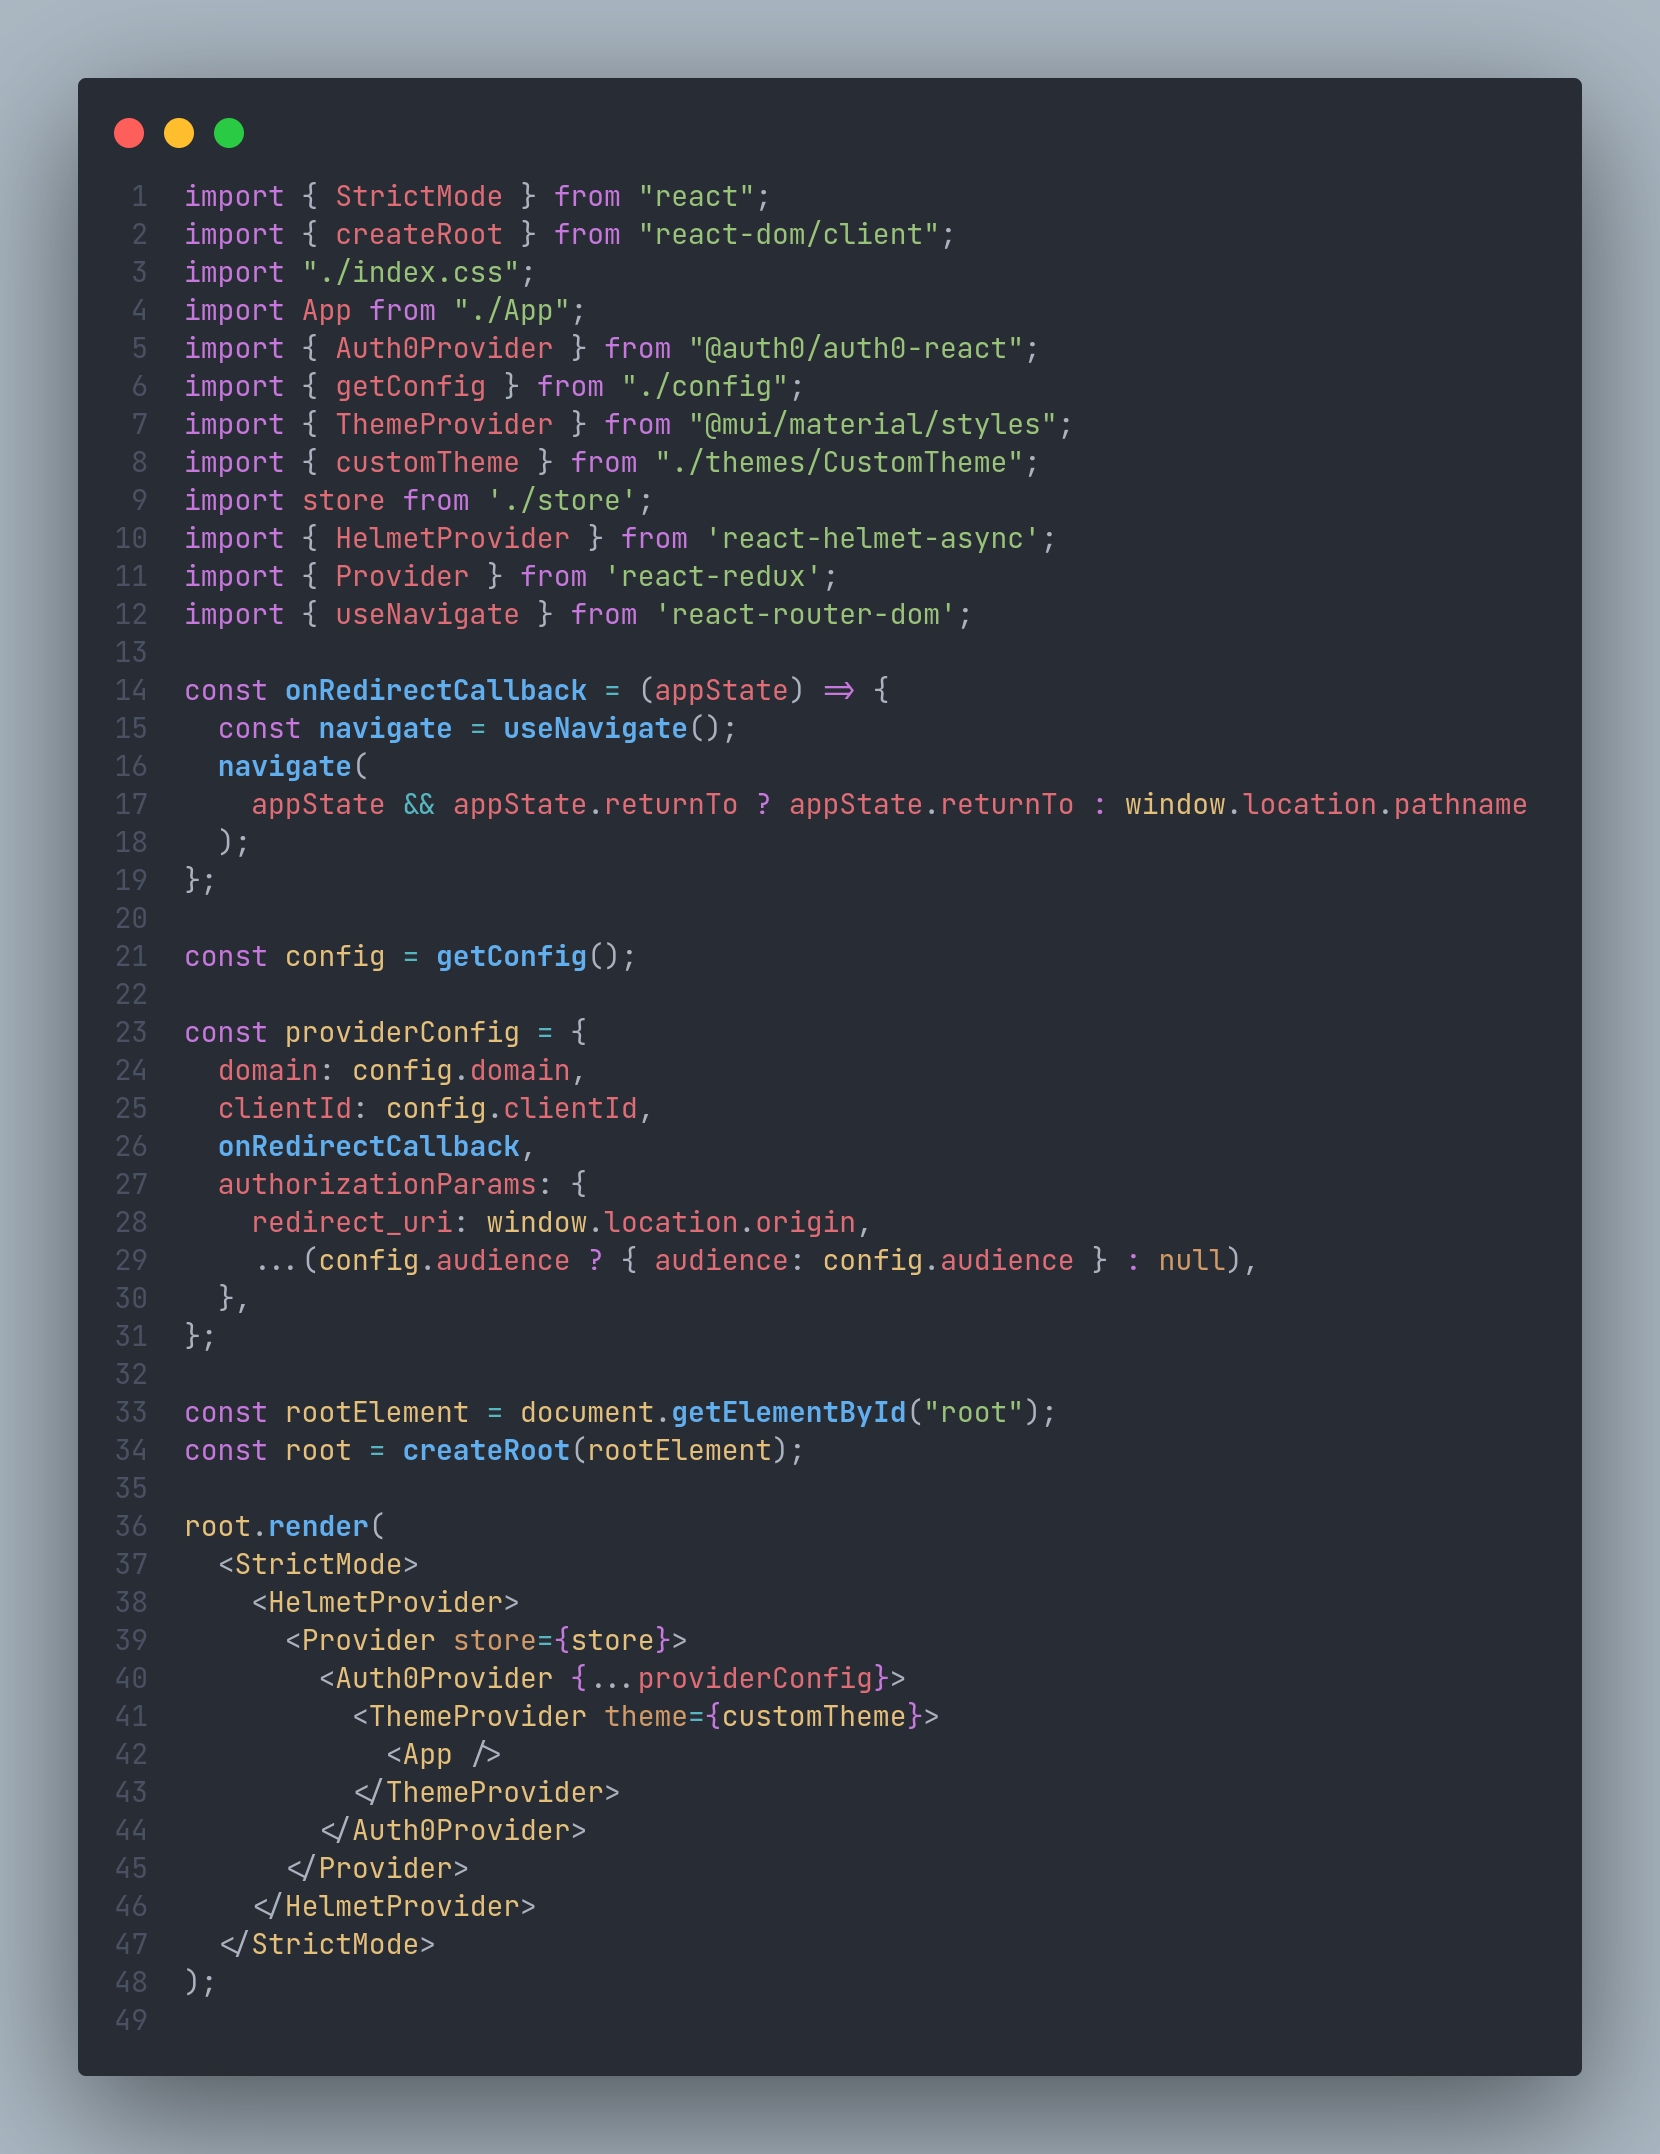
\includegraphics[width=150mm,scale=1]{figures/implementation_and_testing/implementation/frontend/index.png}}
            \caption{Index.js}
        \end{figure}
        
        \vspace{0.25cm}
        \newendline The Auth0Provider wrapper has several properties that need to be configured. The properties are domain, clientID, redirectURI, audience, and onRedirectCallback. The domain property is the domain of the Auth0 application. The clientID property is the client ID of the Auth0 application. The redirectURI property is the URL that Auth0 will redirect the user to after the user has been authenticated. The audience property is the audience of the Auth0 application. The onRedirectCallback property is the callback function that will be called after the user has been authenticated. All of these properties are passed down as a prop using providerConfig constant.
        
        \vspace{0.25cm}
        \newendline Now that the setup is done, let's take a look at logging in. The login process is handled by the LandingPage component. The LandingPage component is responsible for displaying the login page and handling the login process.  The LandingPage component has a button that when clicked, it will call the loginWithRedirect method. The loginWithRedirect method is a method provided by the Auth0 SDK. The loginWithRedirect method is responsible for redirecting the user to the Auth0 login page. Once the user is redirected to the Auth0 login page, the user will be asked to enter their credentials. After the user has entered their credentials, Auth0 will redirect the user to the frontend. The frontend will then call the onRedirectCallback method. The onRedirectCallback method is a method provided by the Auth0 SDK. The onRedirectCallback method is responsible for handling the authentication process. The onRedirectCallback method redirects the user to the homepage if the user has been authenticated successfully. The onRedirectCallback method redirects the user to the login page if the user has not been authenticated successfully.

        \begin{figure}[H]
            \centerline{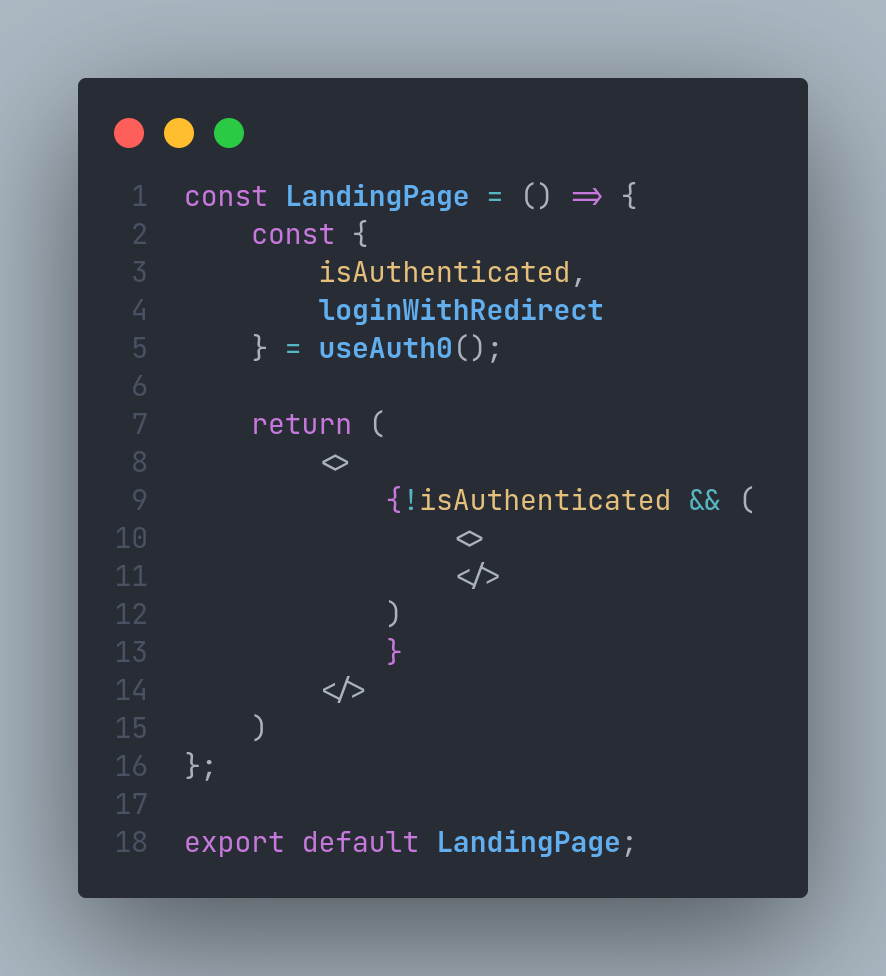
\includegraphics[width=150mm,scale=1]{figures/implementation_and_testing/implementation/frontend/login.png}}
            \caption{Landing Page - Login Code Block}
        \end{figure}

        \vspace{0.25cm}
        \newendline The useAuth0 hook is a custom hook that is used to access the Auth0 SDK. The useAuth0 hook offers a variety of methods that can be used to interact with the Auth0 SDK including those mentioned above. Another useful property is isAuthenticated, which is a boolean value that indicates whether or not the user is authenticated. The isAuthenticated property is used to determine whether or not the user is authenticated. If the user is authenticated, the user will be redirected to the homepage. If the user is not authenticated, the user will be redirected to the login page.
        
        \vspace{0.25cm}
        \newendline Next, let's have a look at the logout process. The logout process is handled by the NavBar component. The NavBar component is responsible for displaying the navigation bar and handling the logout process. The NavBar component has a user profile icon that when clicked, it will show a menu of option, including visiting profile and loging out. When logout is clicked, it will call the logoutWithRedirect method. The logoutWithRedirect method is a method provided by the Auth0 SDK. The logoutWithRedirect method is responsible for redirecting the user to the Auth0 logout page. After the user has has logged out, Auth0 will redirect the user to the frontend. The frontend will then redirects the user to the login page if the user has been logged out successfully.

        \begin{figure}[H]
            \centerline{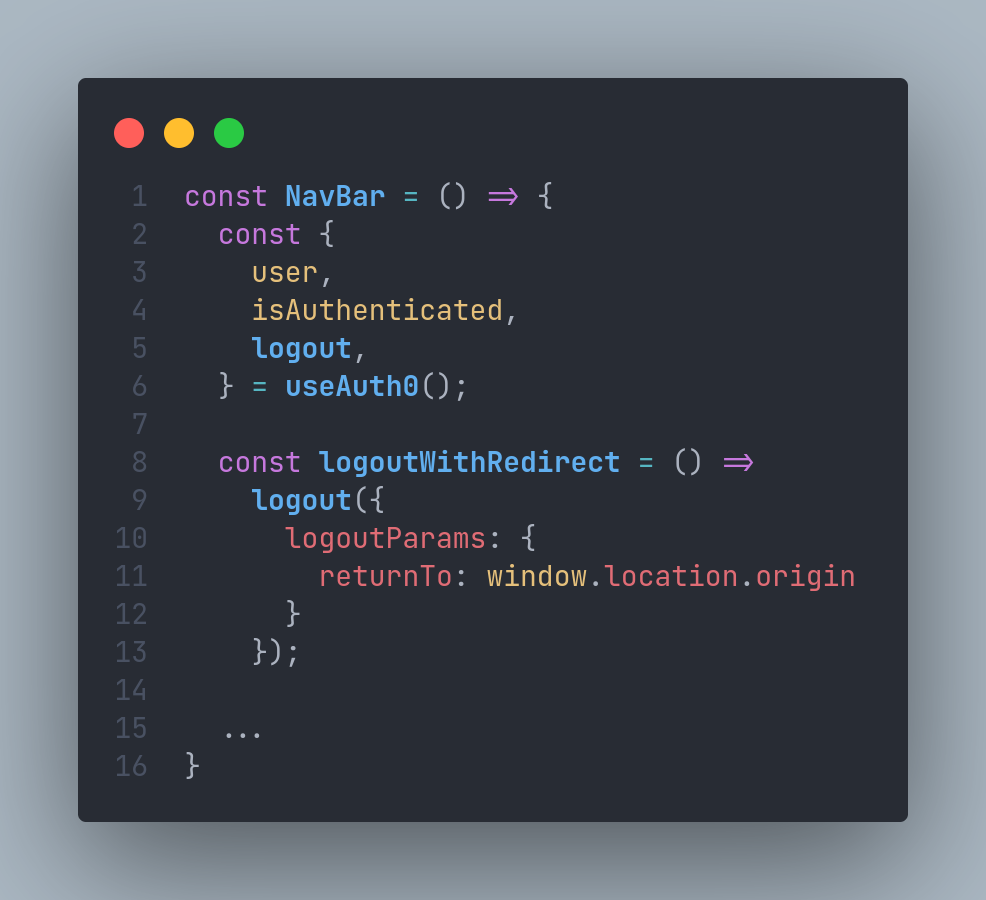
\includegraphics[width=150mm,scale=1]{figures/implementation_and_testing/implementation/frontend/logout.png}}
            \caption{NavBar - Logout Code Block}
        \end{figure}

        \clearpage
        \newendline The Auth0 setup and configurations, login, and logout have been discussed in this section. Before Authorization is discussed, it is essential to discuss and understand how a logged in user is keeping their sessions. The process of setting up a current user is discussed below here.

        \vspace{0.25cm}
        \newendline The App component is the entry point of the application. The App component is responsible for setting up the application and rendering the application. The App component is where the set up of the currentUser is done.
        First, the StdcApiOpenAPI is configured, more on this in the coming sections. The StdcApiOpenAPI is is used to communicate with the backend.
        Then, the Auth0 SDK is used to get the access token silently. The access token is used to authenticate the user. The access token is used to authenticate the user by passing it to the backend. The backend will then verify the access token and return the user if the access token is valid. The access token is stored in the local storage to be used later with every request to the backend.
        Since the current user is set, the application can now be rendered. The current user can be accessed anywhere as long as they are authenticated.

        \begin{figure}[H]
            \centerline{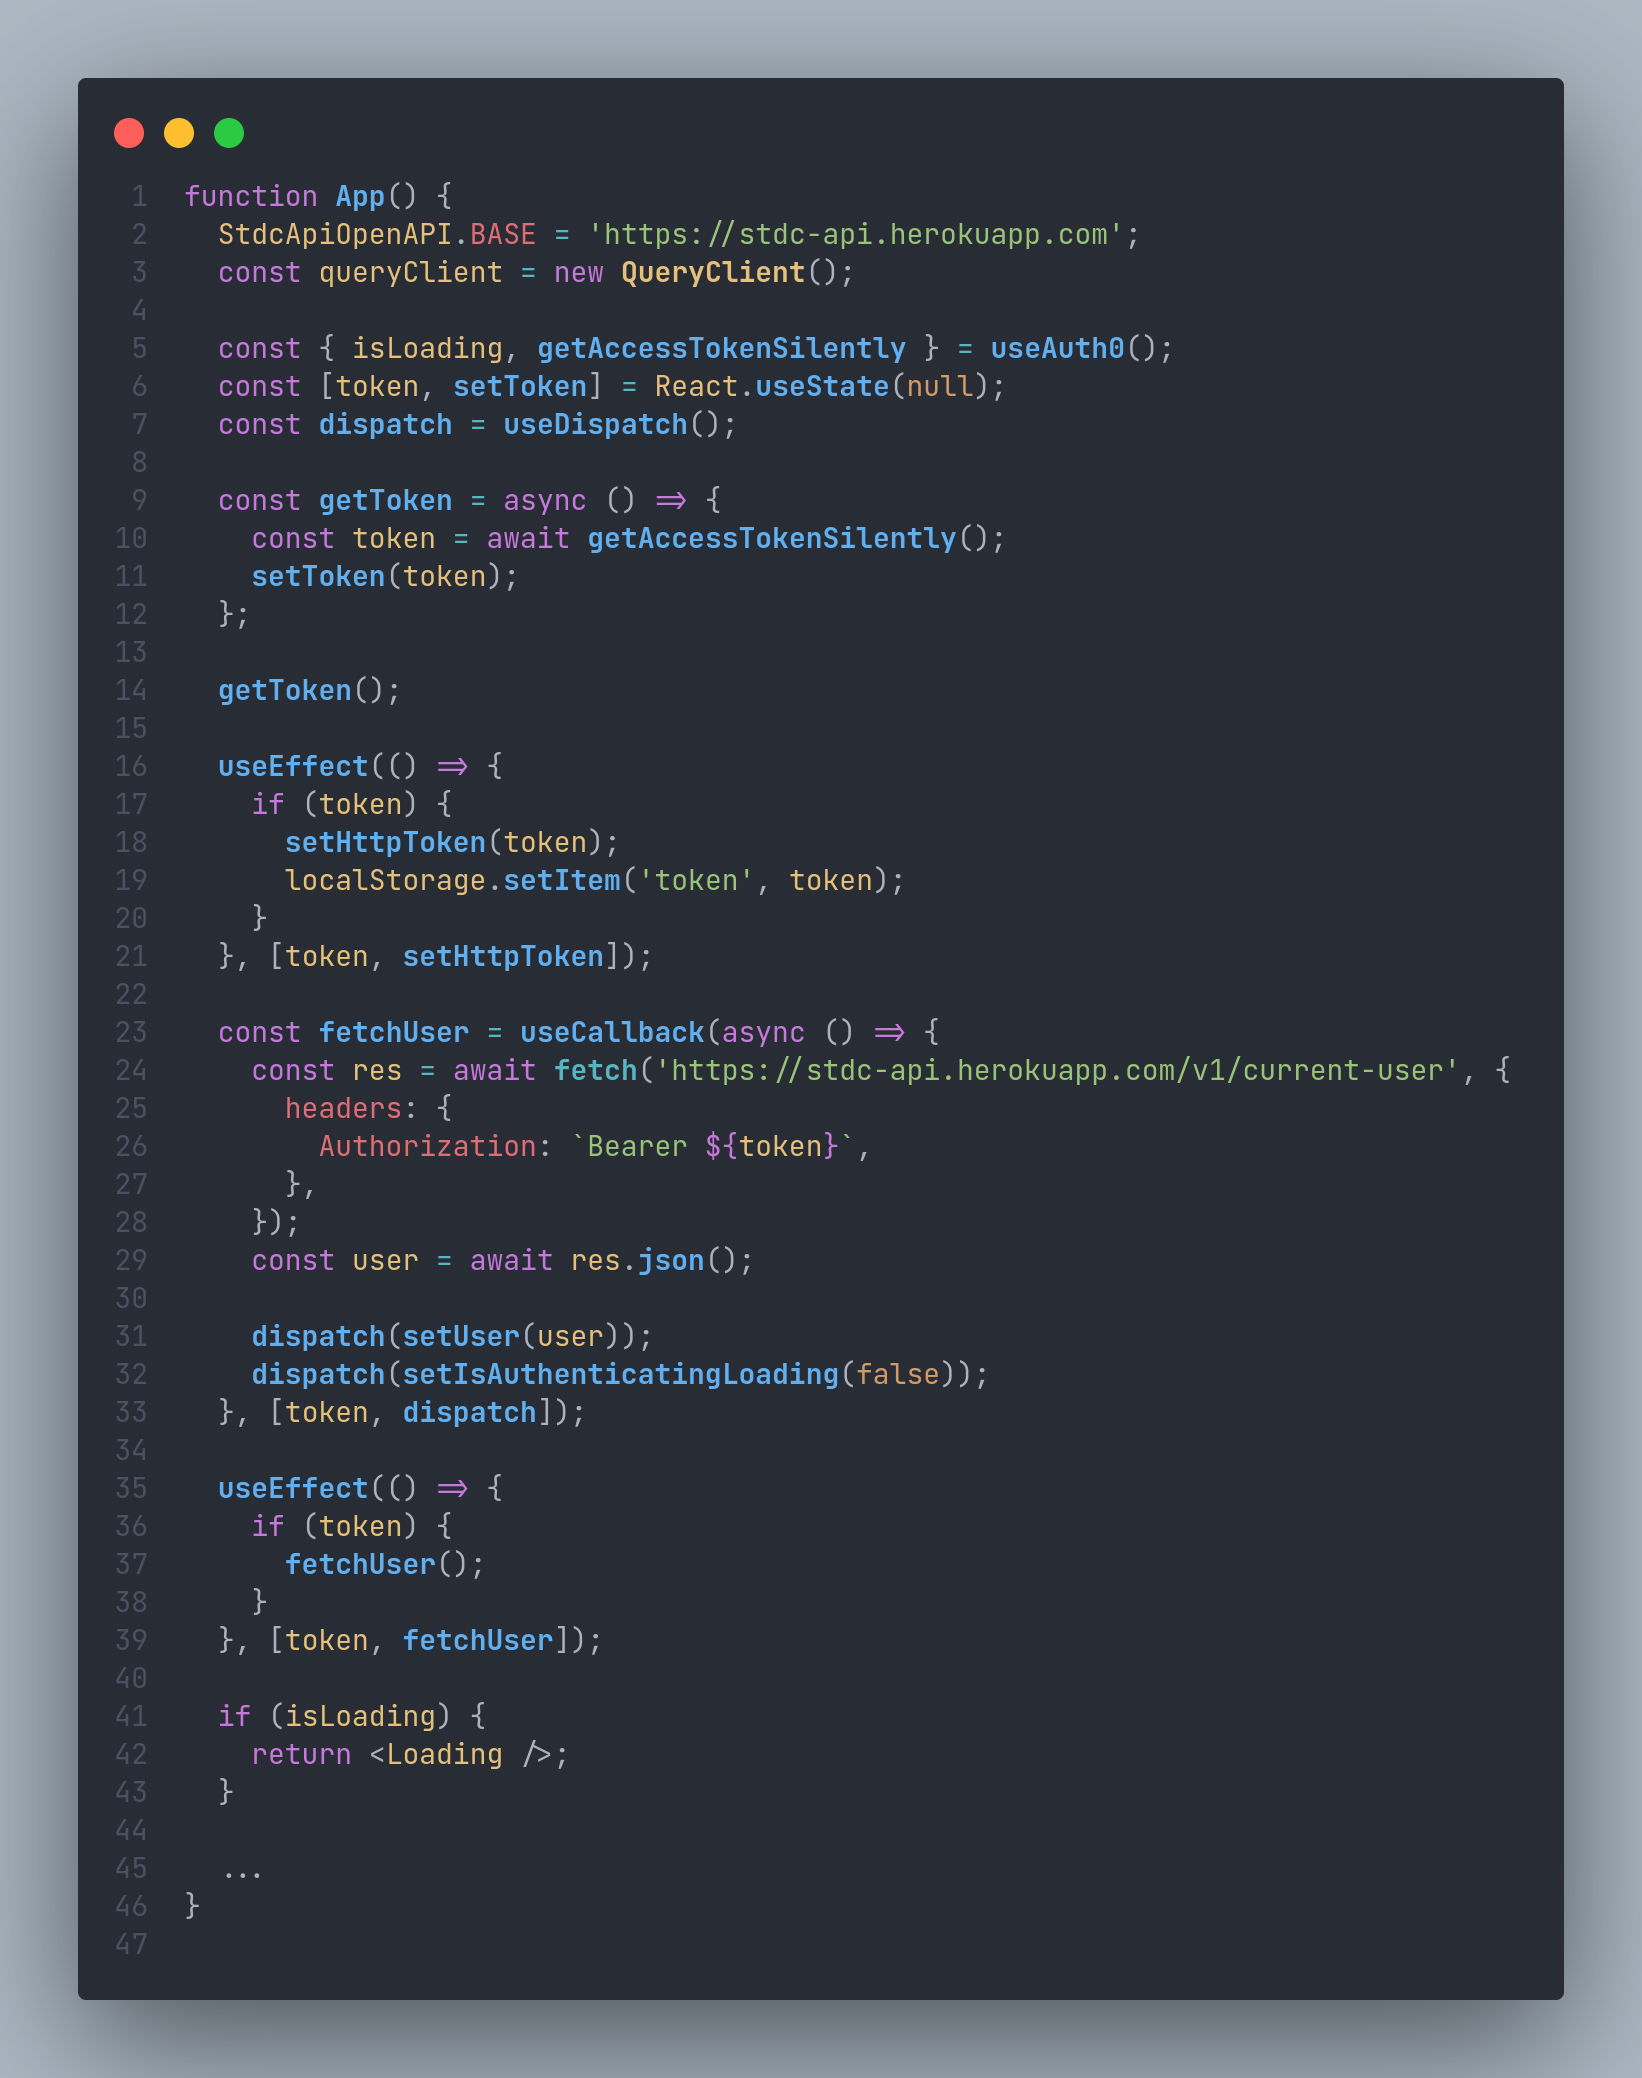
\includegraphics[width=150mm,scale=1]{figures/implementation_and_testing/implementation/frontend/app.png}}
            \caption{App.js}
        \end{figure}
        

        \vspace{0.25cm}
        \newendline As previously mentioned, the backend will be handling authentication for the most part. As for the client side, obtaining the token and keeping the user in a session was the objective. There are more details when it comes to authentication, but the mentioned parts are the most important parts of the authentication process. The other parts of the authentication process are not mentioned in this section because they can be abstracted away. In brief, now we know how authentication works. Next let's take a look onto authorization.

    \clearpage



%%%%%%%%%%%%%%%%%%%%%%%%%%%%%%%%%%%%%%%%%%%%%%%%%%%%%%%%%%%%%%%%%%
%%%%%%%%%%%%%%%%%%%%%%%%%%%%%%%%%%%%%%%%%%%%%%%%%%%%%%%%%%%%%%%%%%
%%%%%%%%%%%%%%%%%%%%%%%%%%%%%%%%%%%%%%%%%%%%%%%%%%%%%%%%%%%%%%%%%%
%%%%%%%%%%%%%%%%%%%%%%%%%%%%%%%%%%%%%%%%%%%%%%%%%%%%%%%%%%%%%%%%%%




    \vspace{0.25cm}
    \newendline \textbf{\textit{Authorizations}}\newendline
        The Student Talent Development Center (STDC)'s client (frontend) routes are managed by the react-router-dom library. The react router library provides a BrowserRouter component that wraps the entire application.The BrowserRouter component is responsible for managing the application's routes and rendering the appropriate components based on the current route.Usually React Router DOM requires set of routes to be defined in a tree structure, where each route can have a parent route, and a list of child routes.The App.js file is the entry point of the application after Index.js, and it is where the BrowserRouter component is defined.In order to seprate the concerns, the STDC has its route defined in another place. Then it imports them to the RouterProvider component, and passes them to the BrowserRouter component.
        
        \begin{figure}[H]
            \centerline{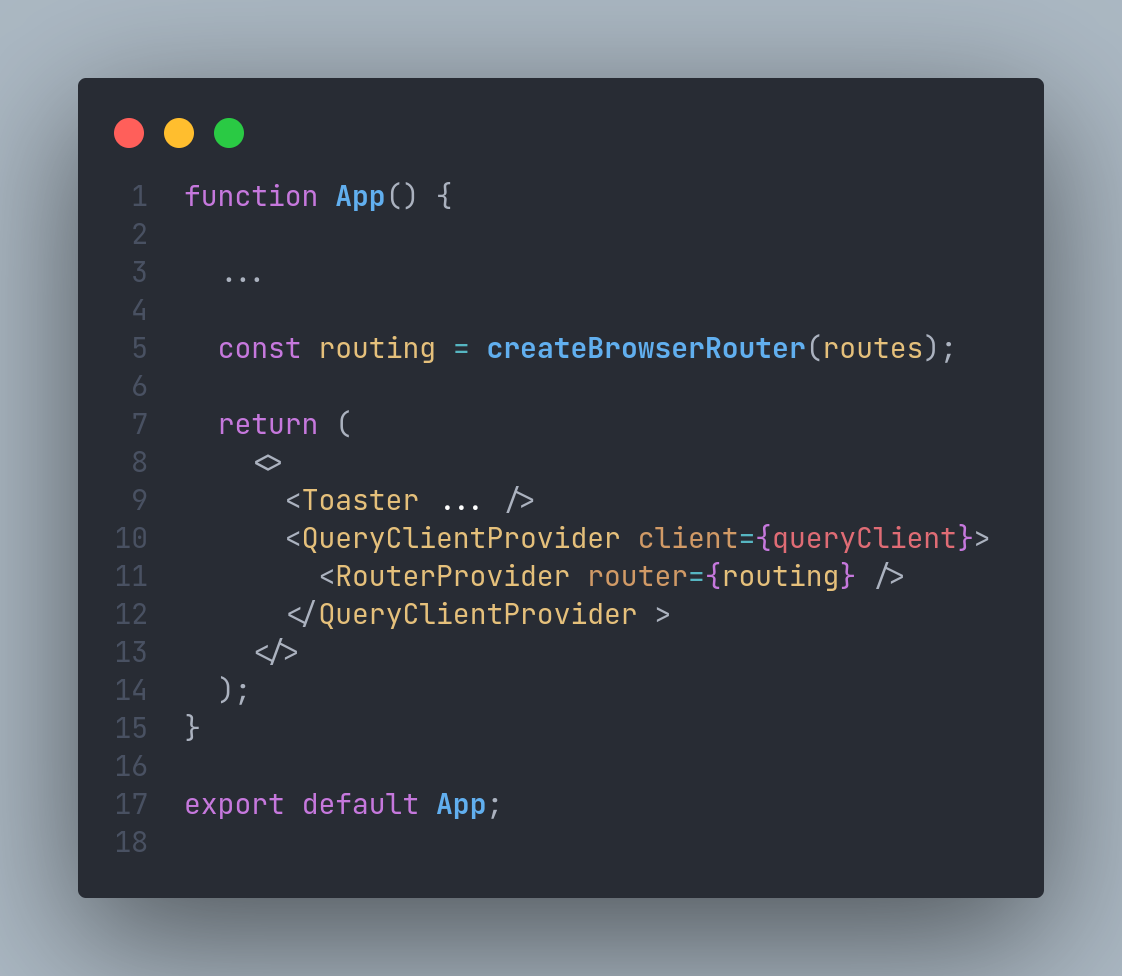
\includegraphics[width=150mm,scale=1]{figures/implementation_and_testing/implementation/frontend/approutes.png}}
            \caption{Routes - App.js}
        \end{figure}

        \vspace{0.25cm}
        \newendline The routes are defined in the routes.js file. The routes are defined in a tree structure, where each route can have a parent route, and a list of child routes. There are two types of routes in the STDC client, protected routes, and public routes. The public routes are the routes that do not require the user to be authenticated to access them. Since STDC is by nature a protected application, the public routes are only the login and the static pages like the 404 page. The protected routes are the routes that require the user to be authenticated to access them. The protected routes are defined in the protectedRoutes array. Despite the fact that the STDC requires authentication to access any of its routes, it also requires authorization to access some of its routes. Each route has a property called "roles", which is an array of strings that represent the roles that are allowed to access the route. The roles are defined in the currentUser object, which is a part of the user slice in the Redux store more on this later. When a user tries to access a route, first the user's roles are checked against the roles of the route, if the user's roles include one of the roles of the route, then the user is authorized to access the route. If the user is not authorized to access the route, then the user is redirected to 403 Forbidden page. In case that the user is not authenticated, then the user is redirected to 401 Unauthorized page. If the route does not exist, then the user is redirected to 404 Not Found page. All of these static pages, 401, 403, and 404 are public, and offer the user to navigate to the home page, or to login page if not authenticated.

        \begin{figure}[H]
            \centerline{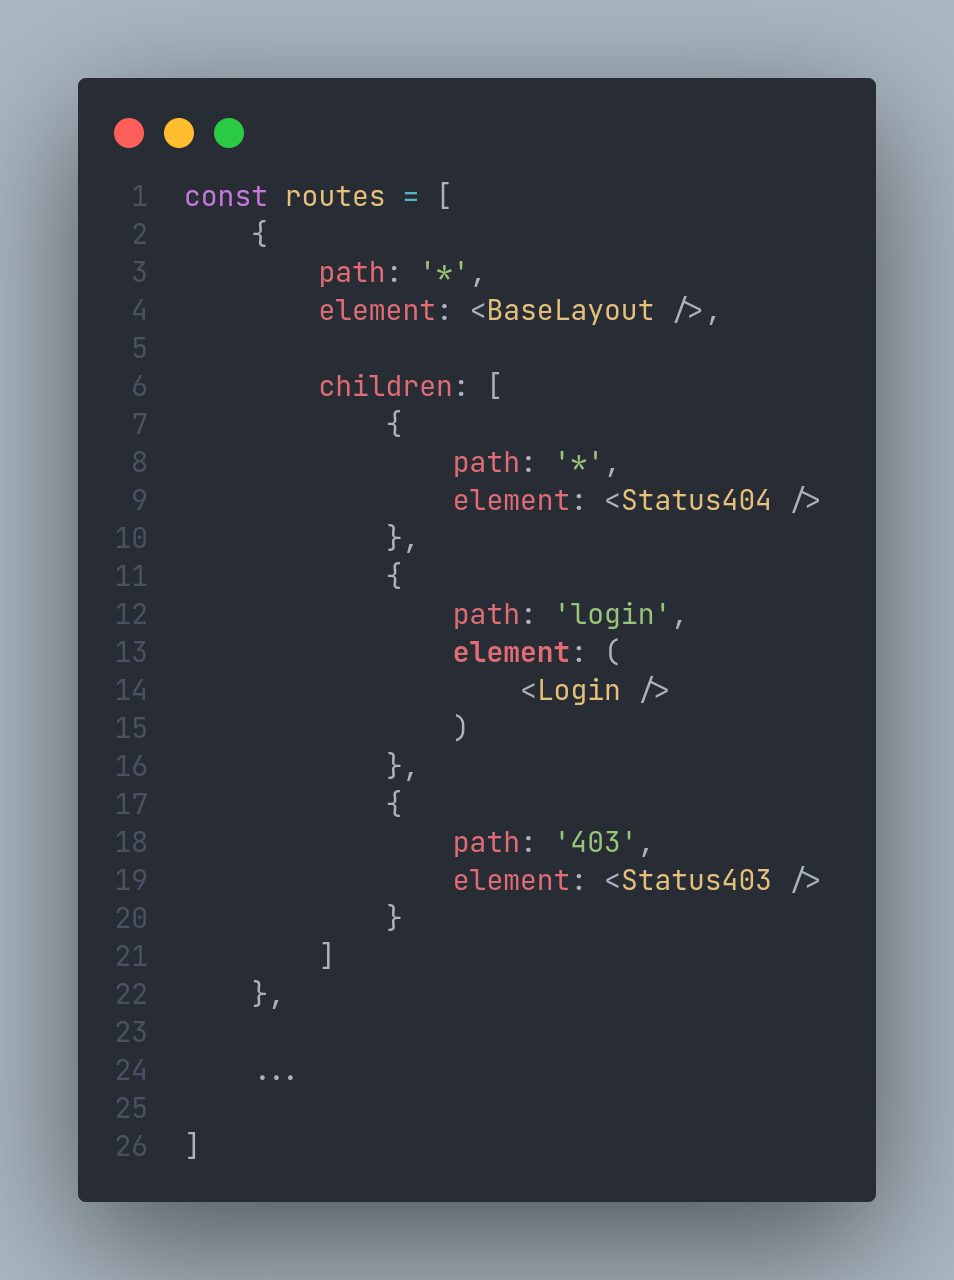
\includegraphics[width=150mm,scale=1]{figures/implementation_and_testing/implementation/frontend/public_routes.png}}
            \caption{Public Routes - routes.js}
        \end{figure}

        \begin{figure}[H]
            \centerline{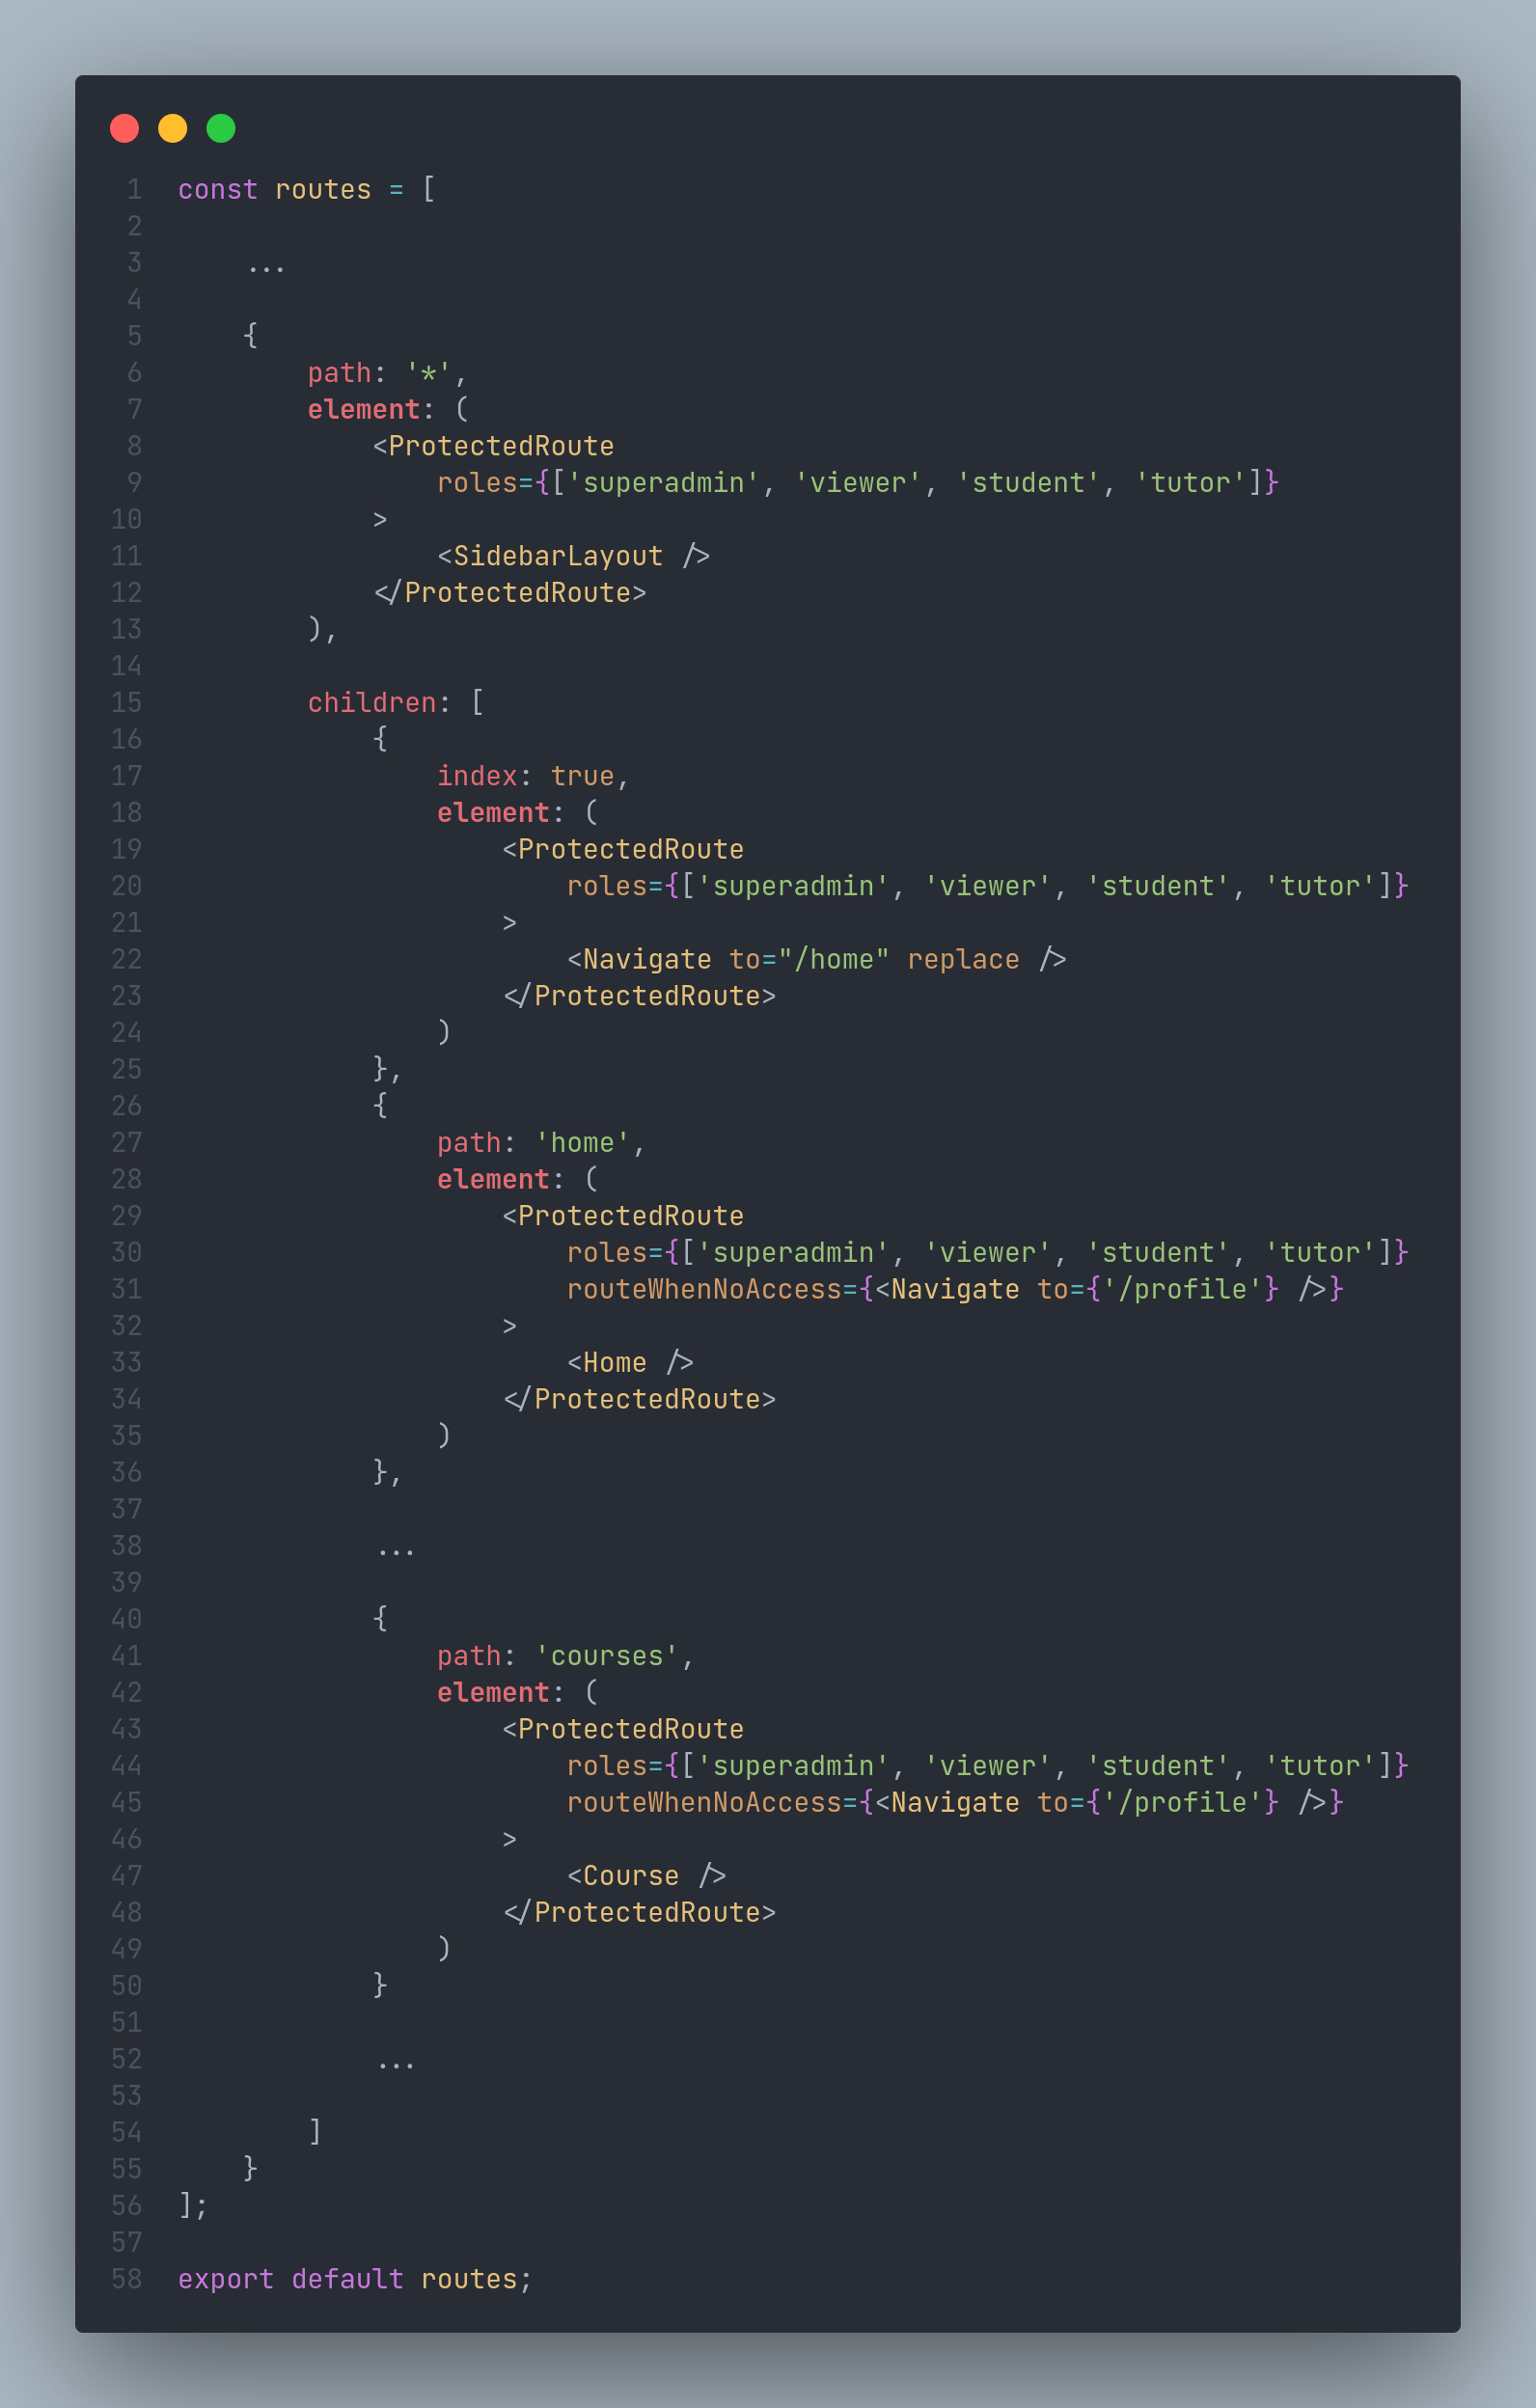
\includegraphics[width=150mm,scale=1]{figures/implementation_and_testing/implementation/frontend/private_routes.png}}
            \caption{Protected Routes - routes.js}
        \end{figure}

        \begin{figure}[H]
            \centerline{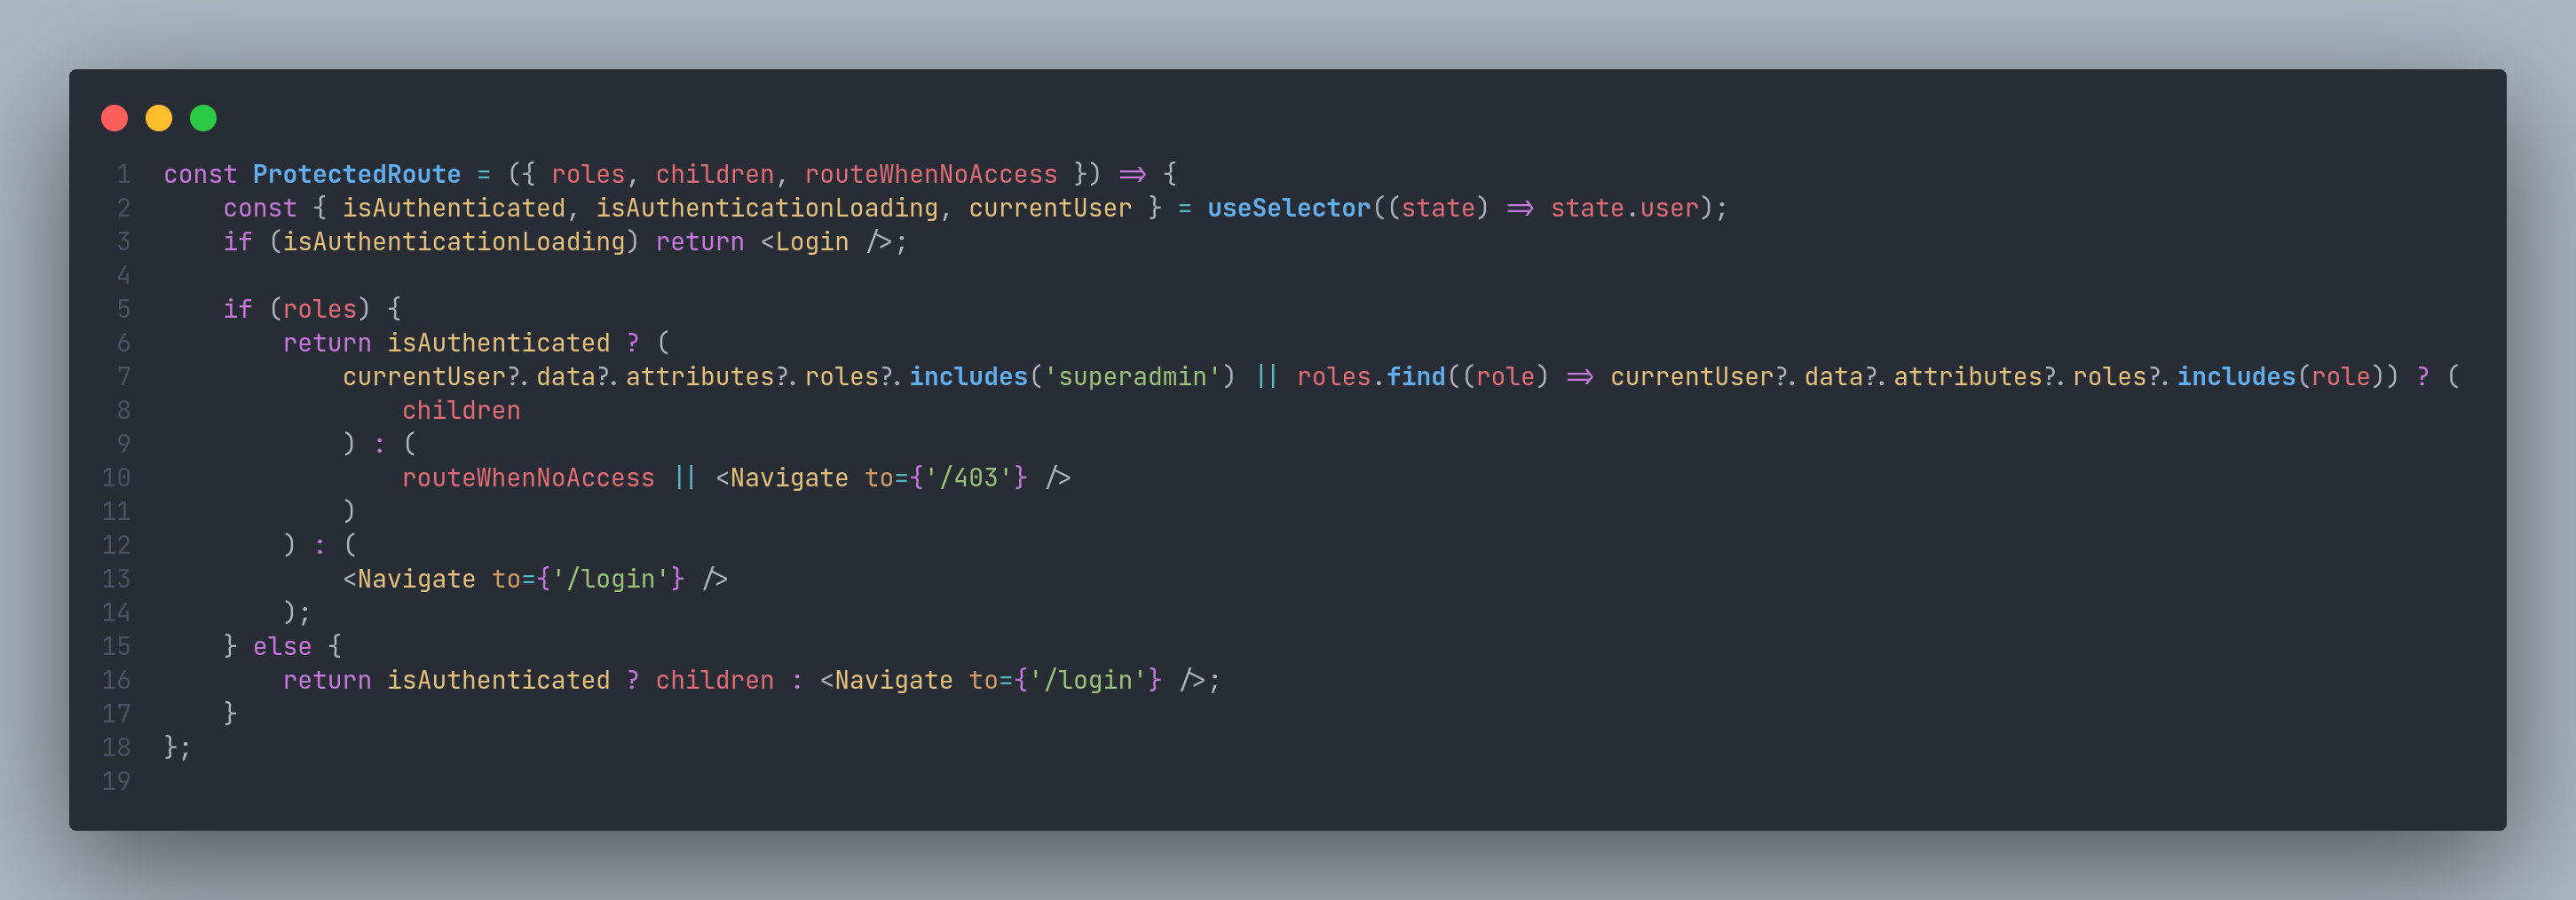
\includegraphics[width=150mm,scale=1]{figures/implementation_and_testing/implementation/frontend/protected_routes.png}}
            \caption{Protected Routes - hasAccessTo Usage}
        \end{figure}

        \vspace{0.25cm}
        \newendline In the routes file, there is a function called hasAccessTo, which is responsible for checking if the user is authorized to access a route. The hasAccessTo function takes an object as an argument, and the object can have two properties, permission, and roles. The permission property is a string that represents the permission that the user needs to access the route. The roles property is an array of strings that represents the roles that are allowed to access the route. The hasAccessTo function checks if the user's roles include the permission, or one of the roles of the route. If the user's roles include the permission, or one of the roles of the route, then the user is authorized to access the route. If the user's roles do not include the permission, or one of the roles of the route, then the user is not authorized to access the route. The hasAccessTo function is a utility function that is used in many places in the STDC client, and it is used to check if the user is authorized to access a route, or to access a component.

        \begin{figure}[H]
            \centerline{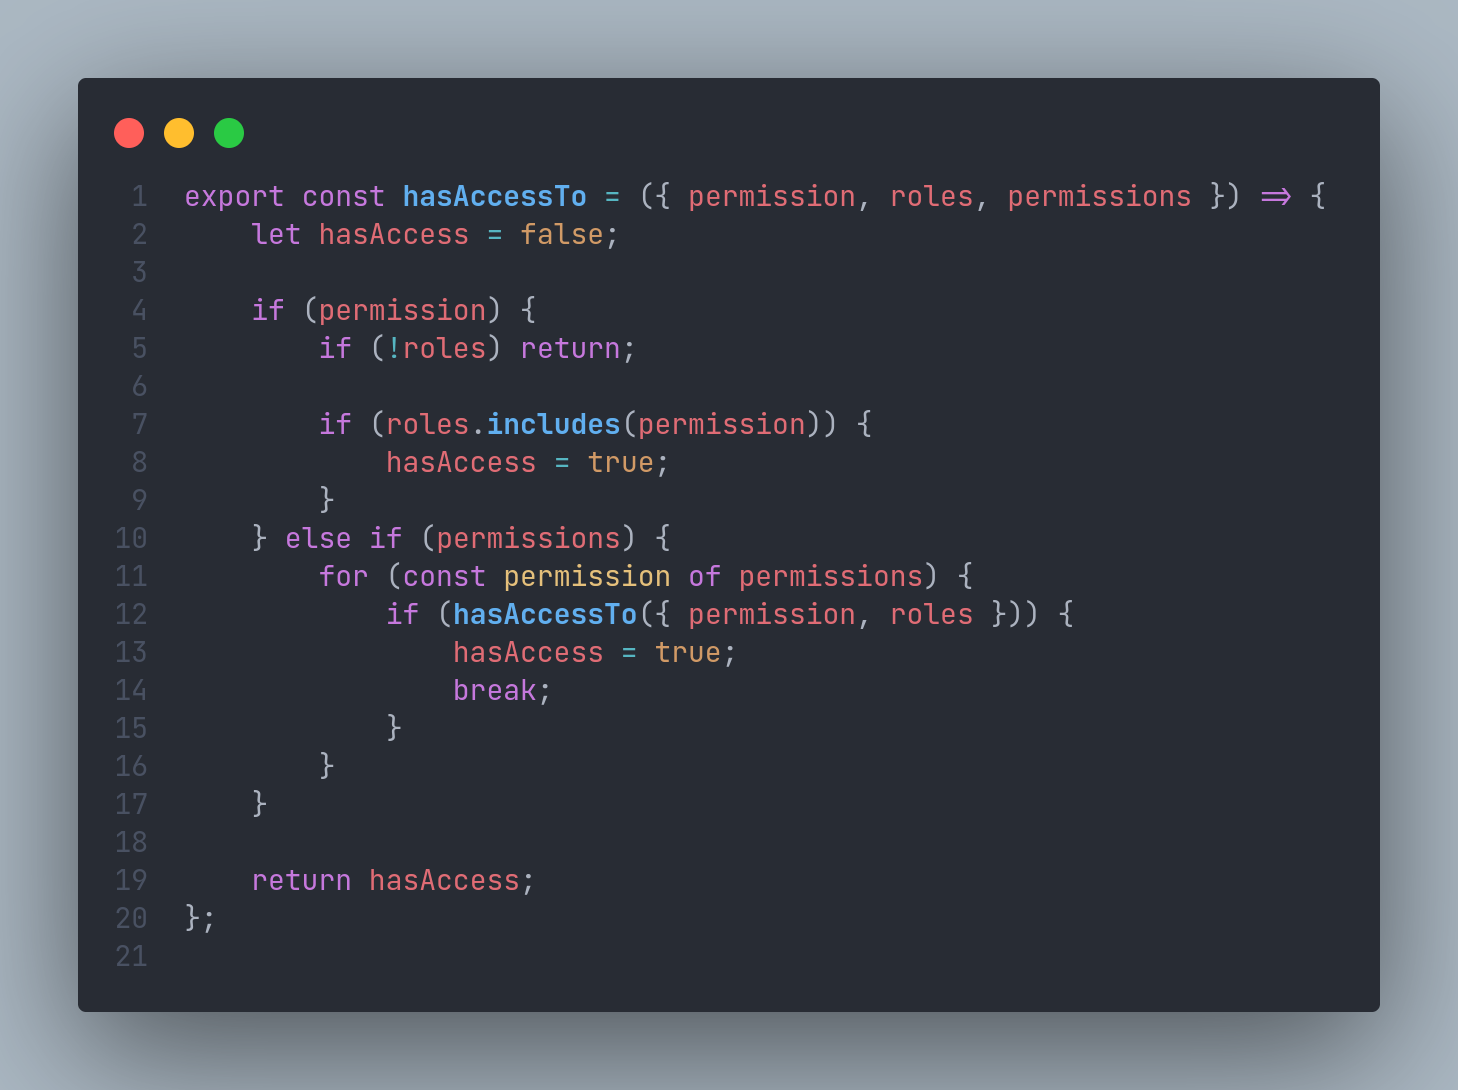
\includegraphics[width=150mm,scale=1]{figures/implementation_and_testing/implementation/frontend/hasAccessTo.png}}
            \caption{hasAccessTo}
        \end{figure}

        \vspace{0.25cm}
        \newendline Below is an example of how hasAccessTo is used in the STDC client. The example is from the Sidebar component, which is the component that renders the sidebar of the application. In the Sidebar component, there is a list of clickable items, each item represents a route in the application. Depending on the user's roles, some of the items are hidden, and some of the items are shown. The below block of code, shows how the hasAccessTo function is used to check if the user is authorized to access the courses route. Only if the user's roles include the superadmin role, then the courses item is shown in the sidebar. Else, the courses item is hidden from the sidebar.

        \begin{figure}[H]
            \centerline{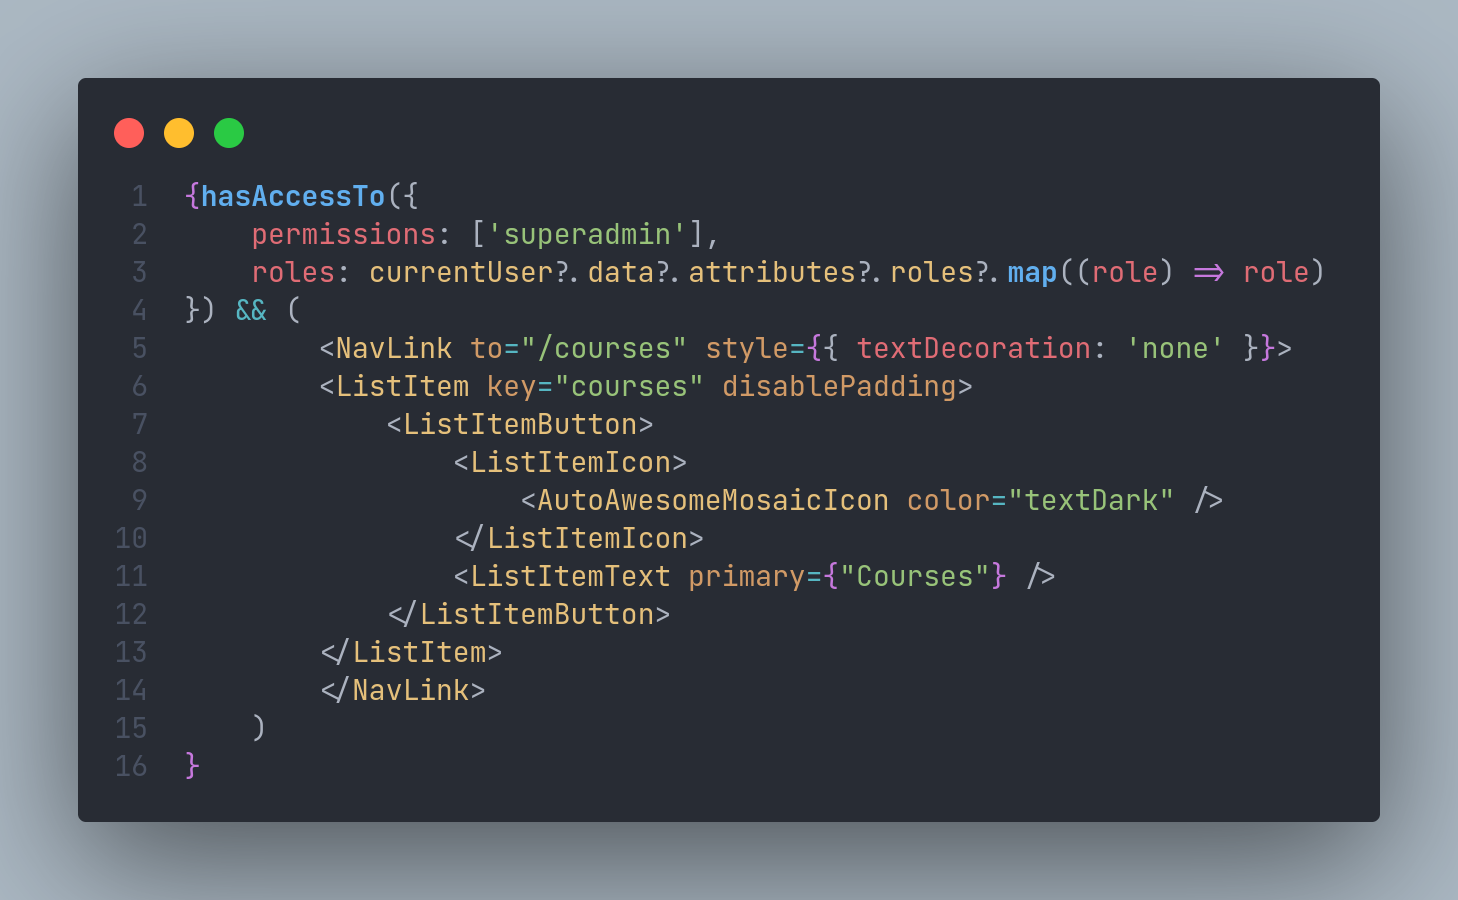
\includegraphics[width=150mm,scale=1]{figures/implementation_and_testing/implementation/frontend/hasAccessTo-Sidebar.png}}
            \caption{hasAccessTo - Sidebar Example}
        \end{figure}

        \vspace{0.25cm}
        \newendline Another example of how hasAccessTo is used in the STDC client, is in the Show Session component. The Show Session component is the component that renders the a specific session's page. In the session page, there are a list of tabs, each tab represents a panel in the session page. Not all of the tabs are shown to the user. Depending on the user's roles, some of the tabs are hidden, and some of the tabs are shown same as the sidebar. The below block of code, shows how the hasAccessTo function is used to check if the user is authorized to access a tab.

        \begin{figure}[H]
            \centerline{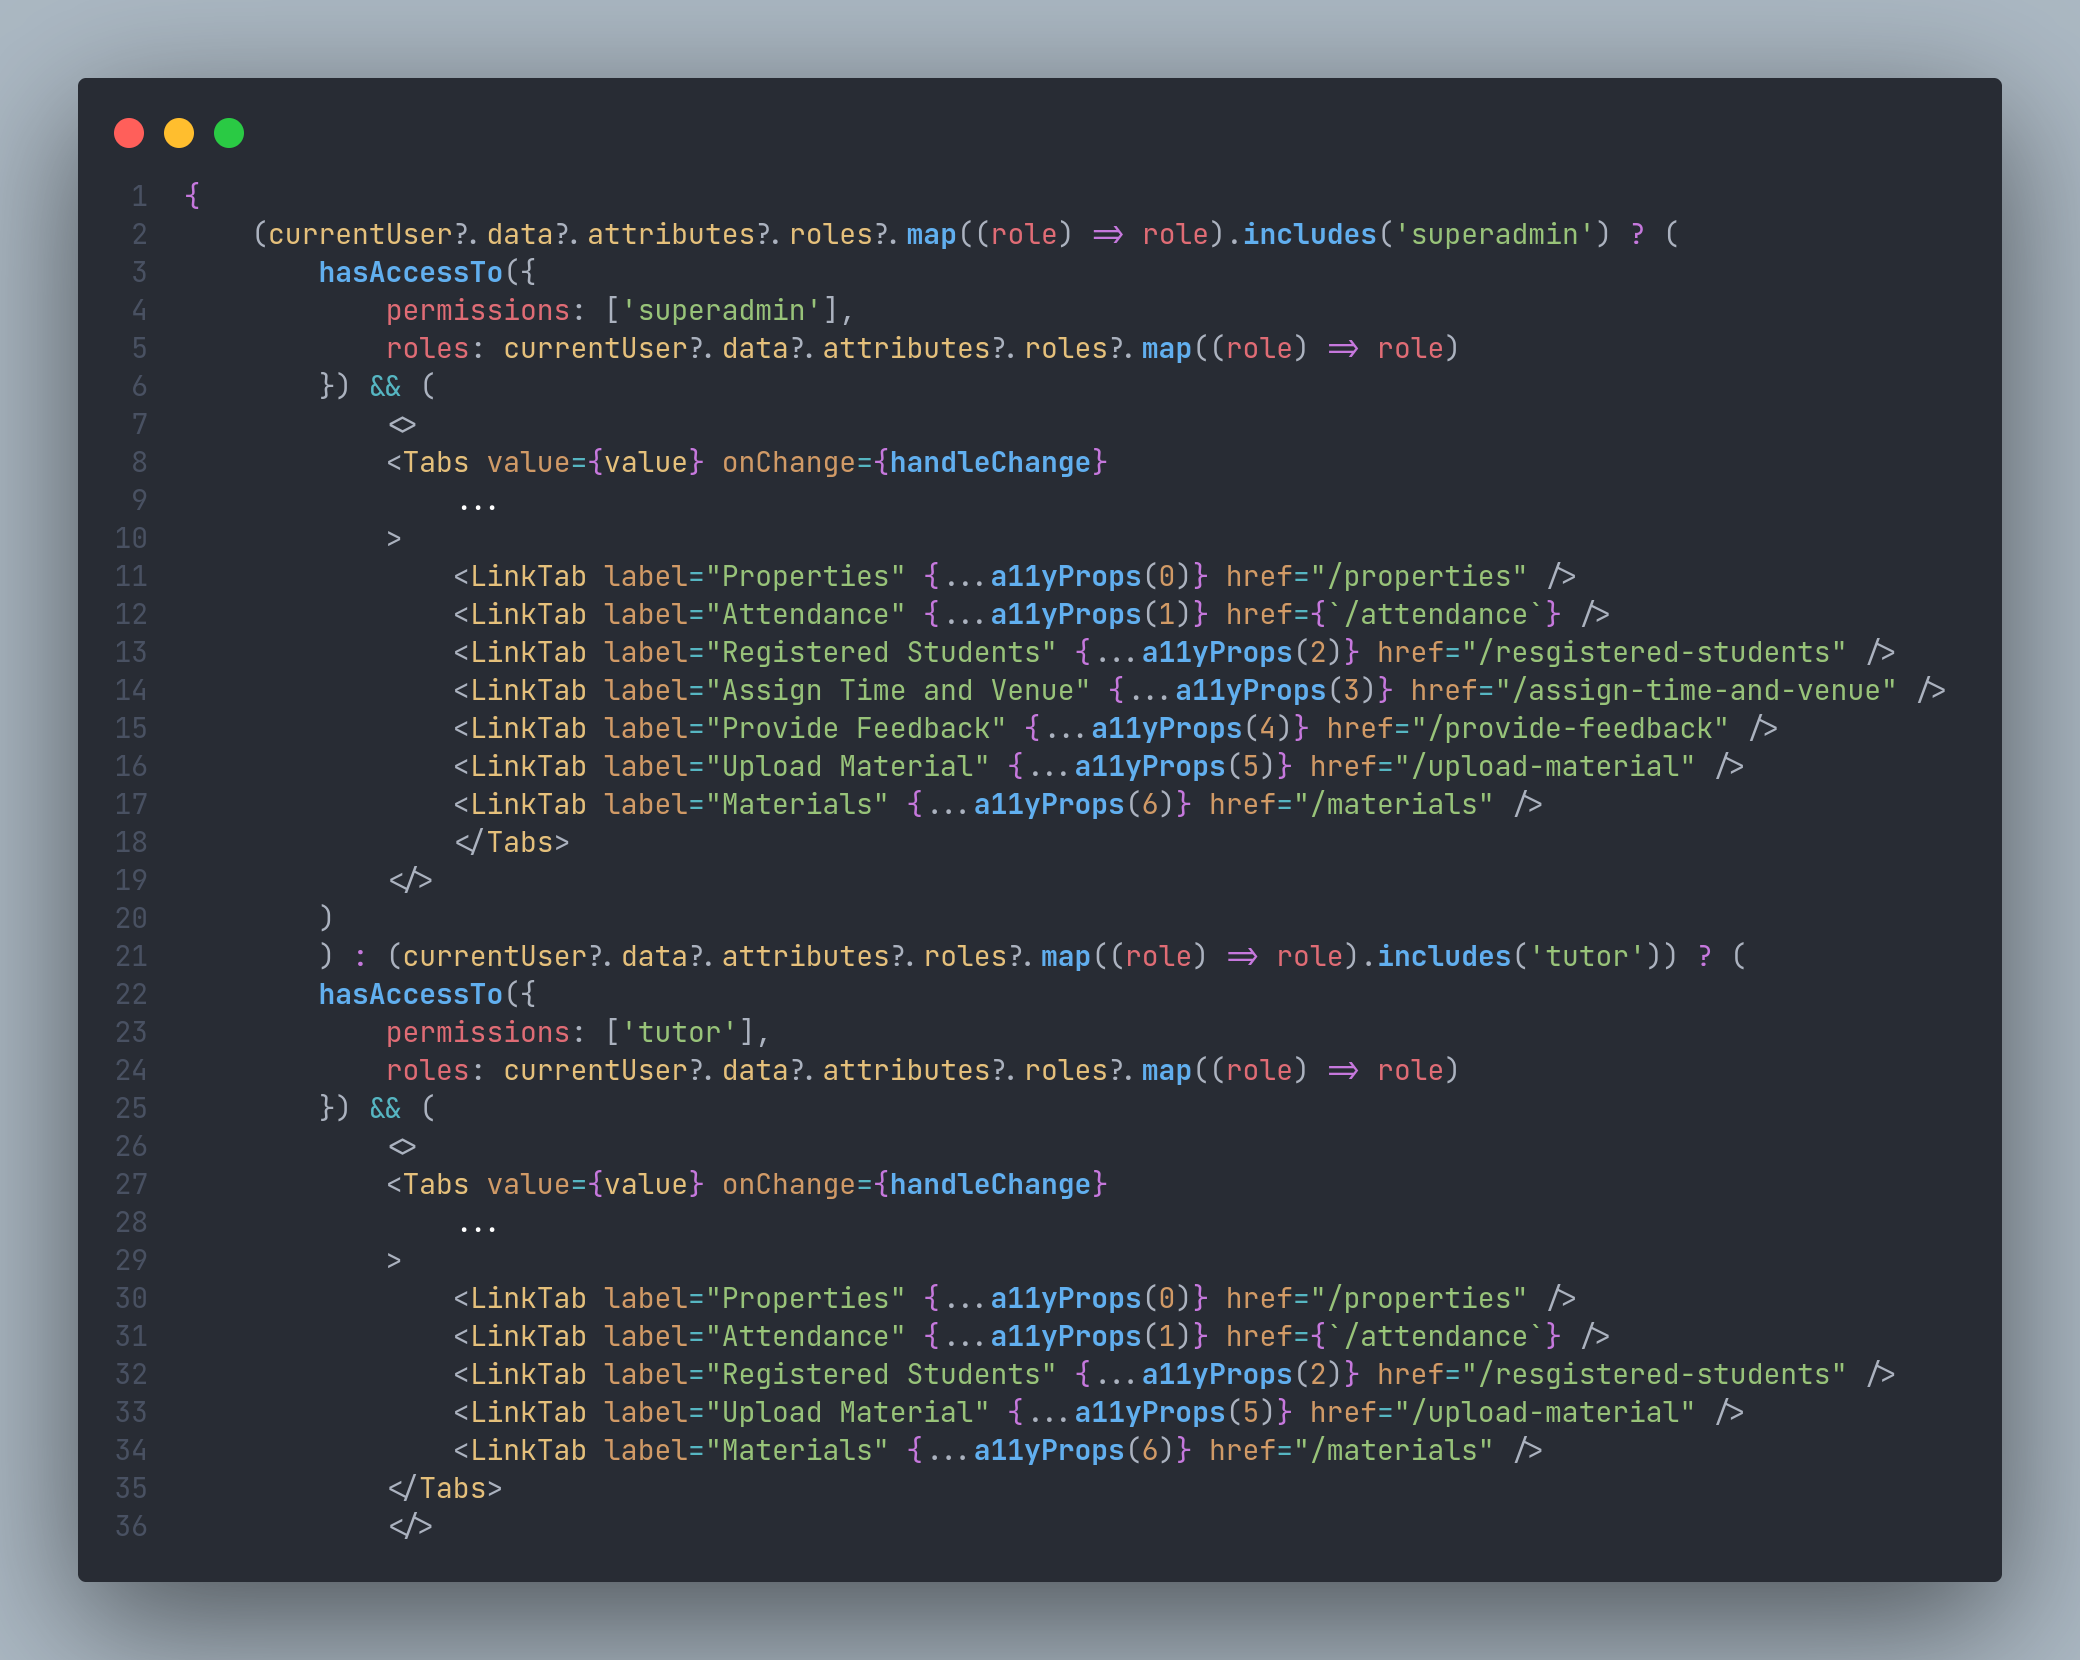
\includegraphics[width=150mm,scale=1]{figures/implementation_and_testing/implementation/frontend/hasAccessTo-Panel-1.png}}
            \caption{hasAccessTo - Panel Example Part 1}
        \end{figure}

        \begin{figure}[H]
            \centerline{\includegraphics[width=150mm,scale=1]{figures/implementation_and_testing/implementation/frontend/hasAccessTo-Panel-2.png}}
            \caption{hasAccessTo - Panel Example Part 2}
        \end{figure}

        \vspace{0.25cm}
        \newendline Although the authorization that is done in the client side is mostly by hiding the components, and the routes, the STDC client also does through authorization in the server side. The server side authorization is done by checking the user's roles against the permissions of user which have been mentioned in the previous section 'Backend'. The client side also redirects users to the 401, 403, and 404 pages, if the user is not authorized to access a route, or a component.

        \vspace{0.25cm}
        \newendline In terms of security, the STDC client is a protected application, and it requires authentication and authorization to access any of its routes, and components. The way STDC deals with client side security might not be the best way, but it is a very good way to deal with client side security nonetheless.

    \clearpage


%%%%%%%%%%%%%%%%%%%%%%%%%%%%%%%%%%%%%%%%%%%%%%%%%%%%%%%%%%%%%%%%%%
%%%%%%%%%%%%%%%%%%%%%%%%%%%%%%%%%%%%%%%%%%%%%%%%%%%%%%%%%%%%%%%%%%
%%%%%%%%%%%%%%%%%%%%%%%%%%%%%%%%%%%%%%%%%%%%%%%%%%%%%%%%%%%%%%%%%%
%%%%%%%%%%%%%%%%%%%%%%%%%%%%%%%%%%%%%%%%%%%%%%%%%%%%%%%%%%%%%%%%%%


    \vspace{0.25cm}
    \newendline \textbf{\textit{API Communication}}\newendline
        The Student Talent Development Center (STDC) client (frontend) communicates with the backend using the OpenAPI, Axios, Axios Interceptors, and React Query. The OpenAPI is used to generate services that are based on the API, which promotes the efficient and standardized development of software. Axios is a promise-based HTTP client that makes it simple to exchange information between the frontend and the backend of web applications. Interceptors are functions that can be used to intercept requests or responses before they are handled by the application. React Query is a library that makes it simple to fetch, cache, and update data in React applications.  All of these technologies are integrated together to communicate with the backend. Now let's take a look at how the STDC client uses these technologies to communicate with the backend.

        \vspace{0.25cm}
        \newendline The OpenAPI is used to generate services that are based on the API, which is the swagger that the backend have generated. Each schema that the backend have made available in the backend will become available to client on the service generation. The generation of the services is done using the openapi-generator-cli package. The openapi-generator-cli package is a command line interface that can be used to generate services based on the API. The openapi-generator-cli package is configured in the package.json file. The package.json file is the file that contains the configuration of the STDC client.

        \begin{figure}[H]
            \centerline{\includegraphics[width=150mm,scale=1]{figures/implementation_and_testing/implementation/frontend/package-openapi.png}}
            \caption{OpenAPI Command to Generate Services}
        \end{figure}

        \vspace{0.25cm}
        \newendline In order for the above command to work, first the base address of the api needs to be set. This is done in the App.js file. 

        \begin{figure}[H]
            \centerline{\includegraphics[width=120mm,scale=1]{figures/implementation_and_testing/implementation/frontend/app-openapi.png}}
            \caption{OpenAPI Base Address}
        \end{figure}

        \vspace{-0.5cm}
        \newendline Once the command is set in the package.json file, and the base address is set in the App.js file, the services can be generated. The services are generated in the services folder. The services folder is the folder that contains the services that are generated based on the API. The services folder is located in the src folder. The src folder is the folder that contains the source code of the STDC client.

        \begin{figure}[H]
            \centerline{\includegraphics[width=105mm,scale=1]{figures/implementation_and_testing/implementation/frontend/services.png}}
            \caption{Services Folder}
        \end{figure}

        \vspace{-0.5cm}
        \newendline The following figure shows how the services are used to fetch courses from the backend.

        \begin{figure}[H]
            \centerline{\includegraphics[width=145mm,scale=1]{figures/implementation_and_testing/implementation/frontend/services_usage.png}}
            \caption{Services Usage - Get Courses}
        \end{figure}

        \vspace{-0.5cm}
        \newendline The below service is generated by the Open API library. The service is used to allow for sending a post request of a course creation to the backend.
        
        \begin{figure}[H]
            \centerline{\includegraphics[width=130mm,scale=1]{figures/implementation_and_testing/implementation/frontend/services_course.png}}
            \caption{Generated Service - Post Course Endpoint}
        \end{figure}

        \vspace{0.25cm}
        \newendline React Query is another library that is used to communicate with the backend. React Query is a library that makes it simple to fetch, cache, and update data in React applications. React Query is configured in the App.js file as follows:

        \begin{figure}[H]
            \centerline{\includegraphics[width=150mm,scale=1]{figures/implementation_and_testing/implementation/frontend/app-query and interceptor.png}}
            \caption{React Query Configuration}
            \label{fig:app-query}
        \end{figure}

        \vspace{0.25cm}
        \newendline The component of the STDC have access to the React Query using the useQuery hook. The QueryClientProvider context provider is used to provide the React Query to the components. Component of the application use it the useQuery hook directly or through the services. The Services that are generated by the OpenAPI, makes use of React Query, the below example shows the serivces' usage of React Query.

        \begin{figure}[H]
            \centerline{\includegraphics[width=150mm,scale=1]{figures/implementation_and_testing/implementation/frontend/service_query.png}}
            \caption{Services' Query Usage}
        \end{figure}

        \vspace{0.25cm}
        \newendline Axios is a promise-based HTTP client that makes it simple to exchange information between the frontend and the backend of web applications. Axios is configured inside the services and used by the OpenAPI to communicate with the backend. However, Axios has interceptors that can be used to intercept requests or responses before they are handled by the application. Interceptors are useful for a variety of reasons, including handling errors, adding headers to requests, and more. The figure \ref{fig:app-query} shows how the intecepters are configured in the App.js file. The below figure shows how the interceptors are configured in the STDC client.

        \begin{figure}[H]
            \centerline{\includegraphics[width=135mm,scale=1]{figures/implementation_and_testing/implementation/frontend/axios.png}}
            \caption{Axios Interceptors Configuration}
        \end{figure}

        \vspace{0.25cm}
        \newendline The above figure shows that the interceptor for responses is used to intercept responses before they are handled by the application to normalize the responses before they are handled by the application. Another use of this interceptor is to redirect the use to the static pages of 401 and 403 if the user is not authenticated or not authorized to access the requested resource.  The interceptor for requests is used to intercept requests before they are sent to the backend to add the access token to the request headers.  The access token is used to authenticate the user by passing it to the backend.  The backend will then verify the access token and return the requested resource upon authentication.


        \vspace{0.25cm}
        \newendline In this section, we talked about how the above technologies were integrated into the STDC client and
        how they have been utilized to communicate with the backend. Next, we will talk about how the STDC client handles its State Management.

        \clearpage


%%%%%%%%%%%%%%%%%%%%%%%%%%%%%%%%%%%%%%%%%%%%%%%%%%%%%%%%%%%%%%%%%%
%%%%%%%%%%%%%%%%%%%%%%%%%%%%%%%%%%%%%%%%%%%%%%%%%%%%%%%%%%%%%%%%%%
%%%%%%%%%%%%%%%%%%%%%%%%%%%%%%%%%%%%%%%%%%%%%%%%%%%%%%%%%%%%%%%%%%
%%%%%%%%%%%%%%%%%%%%%%%%%%%%%%%%%%%%%%%%%%%%%%%%%%%%%%%%%%%%%%%%%%




    \vspace{0.25cm}
    \newendline \textbf{\textit{State Management}}\newendline
        In the process of developing React applications, state management is an essential component as the application requires the continuous synchronization of data across all of the different components. It is common practice to make use of the Redux library in React applications in order to manage the application's global state. Redux is a predictable state container. Redux makes it possible to organize and update state in a manner that is consistent and predictable by requiring that its users follow a predetermined set of steps. Explanation of how Redux work is not in the scope of this section. However, the STDC client uses Redux to manage its state. The STDC client uses Redux to manage its state in a manner that is consistent with the Redux's best practices. Now, let's take a look at how the STDC client uses Redux to manage its state.

        \vspace{0.25cm}
        \newendline The main structure of the STDC client's redux is as follows:

        \begin{itemize}
            \item The store is the object that holds the application's state.
            \item The reducer is a function that takes the current state and an action as arguments and returns the next state.
            \item The slice is a collection of reducer logic and actions for a single feature of the application's state.
        \end{itemize}

        \vspace{0.25cm}
        \newendline The store is the object that holds the application's state. The store is as follows:

        \begin{figure}[H]
            \centerline{\includegraphics[width=140mm,scale=1]{figures/implementation_and_testing/implementation/frontend/store.png}}
            \caption{Store}
        \end{figure}

        \vspace{0.25cm}
        \newendline STDC also has a rootReducer, which is a function that combines all of the reducers into a single reducer. The rootReducer is defined as follows:

        \begin{figure}[H]
            \centerline{\includegraphics[width=150mm,scale=1]{figures/implementation_and_testing/implementation/frontend/rootReducer.png}}
            \caption{Root Reducer}
        \end{figure}

        \vspace{0.25cm}
        \newendline The STDC client's redux is divided into slices, each slice is responsible for managing a specific part of the application's state. The slices are as follows:

        \begin{enumerate}
            \item user: The user slice is responsible for managing the current user's state. The user's state includes the user's information.
            \item venues: The venues slice is responsible for managing the venues' state. The venues' state includes the venues' information.
            \item courses: The courses slice is responsible for managing the courses' state. The courses' state includes the courses' information.
            \item users: The users slice is responsible for managing the users' state. The users' state includes the users' information.
            \item sessions: The sessions slice is responsible for managing the sessions' state. The sessions' state includes the sessions' information.
            \item feedbacks: The feedbacks slice is responsible for managing the feedbacks' state. The feedbacks' state includes the feedbacks' information.
            \item questions: The questions slice is responsible for managing the questions' state. The questions' state includes the questions' information.
        \end{enumerate}

        \vspace{0.25cm}
        \newendline In general the STDC uses these slices to manage the state of the global filters of the resouce tables.
    
        \vspace{0.25cm}
        \newendline The following is the code of the courses slice. The courses slice is responsible for managing the courses' state. The courses' state includes the courses' information. The courses slice is defined as follows.

        \begin{figure}[H]
            \centerline{\includegraphics[width=150mm,scale=1]{figures/implementation_and_testing/implementation/frontend/course_slice.png}}
            \caption{Course Slice}
        \end{figure}

        \vspace{0.25cm}
        \newendline The course slice consists of setPageIndex, setPageSize, setSortBy, setFilter, and setAllFilters reducers. The setPageIndex reducer is responsible for setting the page index of the courses' page. The setPageSize reducer is responsible for setting the page size of the courses' page. The setSortBy reducer is responsible for setting the sort by of the courses' page. The setFilter reducer is responsible for setting the filter of the courses' page. The setAllFilters reducer is responsible for setting all of the filters of the courses' page. The courses slice also consists of getPageIndex, getPageSize, getSortBy, getFilters, and getCurrentGlobalCourse selectors. Selectors are functions that are used to select a specific part of the state.

        \vspace{0.25cm}
        \newendline The courses slice's reducers are used to keep the state of the resource and then pass the values to react query to fetch the data from the backend based on the state of the resource.

        \vspace{0.25cm}
        \newendline The other slices are defined in a similar manner to the courses slice. In general the STDC uses these slices to manage the state of the global filters of the resouce tables and pages. However, since the STDC continuously communicates with the backend, the STDC client uses Redux for its state management only when needed.

    \clearpage


%%%%%%%%%%%%%%%%%%%%%%%%%%%%%%%%%%%%%%%%%%%%%%%%%%%%%%%%%%%%%%%%%%
%%%%%%%%%%%%%%%%%%%%%%%%%%%%%%%%%%%%%%%%%%%%%%%%%%%%%%%%%%%%%%%%%%
%%%%%%%%%%%%%%%%%%%%%%%%%%%%%%%%%%%%%%%%%%%%%%%%%%%%%%%%%%%%%%%%%%
%%%%%%%%%%%%%%%%%%%%%%%%%%%%%%%%%%%%%%%%%%%%%%%%%`%%%%%%%%%%%%%%%%%



    \vspace{0.25cm}
    \newendline \textbf{\textit{Views}}\newendline
        The Student Talent Development Center (STDC) client (frontend) is a single page application.The STDC client is divided into components, each component is responsible for rendering a specific part of the application.The component directory is located in the src directory. The components directory is the directory that contains the components that the STDC client uses for it views.The Views directory is the directory that contains the views that the STDC client renders as a page.Mainly there are two types of views in the STDC client, the static views, and the dynamic views.The static views are the views that do not require the user to be authenticated to access them.The dynamic views are the views that require the user to be authenticated to access them.The static views are as follows:

        \begin{enumerate}
            \item LandingPage: The LandingPage component is responsible for rendering the login page.
            \item NotFoundPage: The NotFoundPage component is responsible for rendering the not found page when the server return 404.
            \item UnauthorizedPage: The UnauthorizedPage component is responsible for rendering the unauthorized page when the server return 401.
            \item ForbiddenPage: The ForbiddenPage component is responsible for rendering the forbidden page when the server return 403.
        \end{enumerate}

        \vspace{0.25cm}
        \newendline The dynamic views are as follows:

        \begin{enumerate}
            \item App: The App component is the entry point of the application. The App component is responsible for setting up the application and rendering the application.
            \item NavBar: The NavBar component is responsible for rendering the top AppBar.
            \item Sidebar: The Sidebar component is responsible for rendering the sidebar which contains the navigation links.
            \item CoursesPage: The CoursesPage component is responsible for rendering the courses page.
            \item UsersPage: The UsersPage component is responsible for rendering the users page.
            \item SessionsPage: The SessionsPage component is responsible for rendering the sessions page.
            \item FeedbacksPage: The FeedbacksPage component is responsible for rendering the feedbacks page.
            \item QuestionsPage: The QuestionsPage component is responsible for rendering the questions page.
            \item ReleaseNotesPage: The ReleaseNotesPage component is responsible for rendering the release notes page.
        \end{enumerate}



        \vspace{0.25cm}
        \newendline Each dynamic view has their own child views. Let's take the venues view as an example. The venues view consists of the followings:

        \begin{itemize}
            \item schema: The schema is the schema to validate the venues' data on creation and update. Yup is used to validate the venues' data.
            
            \begin{figure}[H]
                \centerline{\includegraphics[width=150mm,scale=1]{figures/implementation_and_testing/implementation/frontend/venue_schema.png}}
                \caption{Venue Schema}
            \end{figure}

            \clearpage
            \newendline The venue schema consists of the name, capacity, status, floor, and availability fields. The name field is a required string field. The capacity field is a required number field. The status field is a string field. The floor field is a string field. The availability field is a string field. Each of the fields has its own validation rules. Capacity field is a number field that is positive, integer, and between 10 and 500. The schema is used to validate the venues' data on creation and update, so when the capacity field is not a number, or is not positive, or is not integer, or is not between 10 and 500, then the schema will return an error. Thus, it will not call the API, unless all the client side validations are passed.
        
            \item all: The all directory is the main Venues Page view. It consists of the following:
                \begin{itemize}
                    \item components/columnns: It is the responsibility of the columns.js file to generate the columns configuration that is utilized in the table view of the venues page. GenerateColumns is a function component that is exported from this file. It accepts setGlobalFilter, setGlobalPageIndex, and currentUser as its parameters.

                    \vspace{0.25cm}
                    \newendline Inside of the component, a number of options arrays are defined, such as statusOptions, floorOptions, and availabilityOptions. These arrays are used to store the various filtering options that can be applied to particular column types.
                    
                    \vspace{0.25cm}
                    \newendline The component gives back an array of column objects that, collectively, define the table's columns. Each column object has properties such as Header, which is the title of the column header, and accessor, which is the data accessor for the cell value. Additionally, each column object can have optional properties such as Filter, which is the filter component for the column, Cell, which is the custom rendering component for the cell, and more.
                    
                    \vspace{0.25cm}
                    \newendline In order to enable filtering based on particular criteria, certain columns make use of custom filter components, such as SearchColumnFilter and AutocompleteColumnFilter. When formatting date values in the createdAt and updatedAt columns, the momentFormat helper function is called upon to do the formatting.
                    
                    \vspace{0.25cm}
                    \newendline Finally, an additional "Actions" column is appended to the returned array of columns in a conditional form if the currently logged-in user possesses the required permissions (the "superadmin" role).
                    
                    \vspace{0.25cm}
                    \newendline This GenerateColumns component plays an important part in defining the columns and their behaviors in the venues table. This gives users the ability to view and interact with the data in an efficient manner.

                        \begin{figure}[H]
                            \centerline{\includegraphics[width=150mm,scale=1]{figures/implementation_and_testing/implementation/frontend/columns-1.png}}
                            \caption{Venue Columns - Part 1}
                        \end{figure}

                        \begin{figure}[H]
                            \centerline{\includegraphics[width=150mm,scale=1]{figures/implementation_and_testing/implementation/frontend/columns-1.png}}
                            \caption{Venue Columns - Part 2}
                        \end{figure}
                    
                    \item PageHeader.js: The PageHeader.js file exports a component with the name PageHeader that has functional significance. It renders a Typography component with the title "Venues" as well as a conditional Button component for the purpose of creating new venues. The hasAccessTo function is used to determine whether or not the currently logged-in user possesses the "superadmin" role's required permissions to view the "create" button. By utilizing the useNavigate hook that is provided by react-router-dom, the Button component, when it is activated, will navigate to the /venues/create route.

                        \begin{figure}[H]
                            \centerline{\includegraphics[width=150mm,scale=1]{figures/implementation_and_testing/implementation/frontend/venue_pageheader.png}}
                            \caption{Venue Page Header}
                        \end{figure}

                    
                    \item Tables.js: The table view of the venues is represented by the Table.js file. This file is a React component. It imports a variety of dependencies and components that are necessary for rendering the table, such as the ReactTable component that is located in the src/components/Table/ReactTable module and the generateColumns function that is located in the./compone- nts/columns file.

                    \vspace{0.25cm}
                    \newendline Using the useState hook, the Table component's internal storage contains a number of state variables that have been defined. These variables are used for managing the deletion and activation of items, as well as tracking the total pages and total items in the table. Additionally, they are used to manage the variables that manage the total pages.
                    
                    \vspace{0.25cm}
                    \newendline The output of calling the generateColumns function results in the table having a wide variety of different column configurations.
                    
                    \vspace{0.25cm}
                    \newendline In order to retrieve the data for the table, the useQuery hook  was utilized. It requires an array of dependencies, which may include the currentPageIndex, currentPageSize, and filters, in addition to an asynchronous function that is responsible for retrieving the data. The data that was retrieved is saved in the variable known as data, and additional variables such as isFetching are used to monitor the loading state of the data.
                    
                    \vspace{0.25cm}
                    \newendline When rendered, the ReactTable component receives a number of props that, collectively, supply the table with its configuration and its data. For the purposes of retrieving and updating the table state, it makes use of the generated columns array, the data that has been fetched, and functions such as getFilters, getPageIndex, getPageSize, and getSortBy. The actions prop renders buttons in a conditional manner, taking into account the permissions of the user. This makes it possible for items to be deactivated or activated.
                    
                    \vspace{0.25cm}
                    \newendline Last but not least, the Table component renders a DeleteModal and an ActivateModal component. These components are employed for confirming and carrying out actions associated to the deactivation of data and activation of data, respectively.
                    
                    \vspace{0.25cm}
                    \newendline The Table.js component, in whole, brings together a number of different functionalities in order to render a table view of the venues. These functionalities include data fetching, pagination, sorting, filtering, and action buttons for managing the venues' current status.

                        \begin{figure}[H]
                            \centerline{\includegraphics[width=150mm,scale=1]{figures/implementation_and_testing/implementation/frontend/table-1.png}}
                            \caption{Venue Table - Part 1}
                        \end{figure}
            
                        \begin{figure}[H]
                            \centerline{\includegraphics[width=150mm,scale=1]{figures/implementation_and_testing/implementation/frontend/table-2.png}}
                            \caption{Venue Table - Part 2}
                        \end{figure}
            
                        \begin{figure}[H]
                            \centerline{\includegraphics[width=150mm,scale=1]{figures/implementation_and_testing/implementation/frontend/table-3.png}}
                            \caption{Venue Table - Part 3}
                        \end{figure}
                        
                    \item Index.js: The Index.js file is the starting point for the page that contains the venues. It imports the PageHeader component and the Table component, and then renders them inside of a container. The PageTitleWrapper component surrounds the PageHeader component, which enables it to provide a formatted page title section. In order to guarantee that the layout is executed correctly, the Table component is nested within a Grid item.

                        \begin{figure}[H]
                            \centerline{\includegraphics[width=150mm,scale=1]{figures/implementation_and_testing/implementation/frontend/venue_index.png}}
                            \caption{Venue Index}
                        \end{figure}
                    
                \end{itemize}
            \item create: A new venue can be created by filling out the form that is represented by the Create component, which is a React component. It gets two props, called defaultNode and onSuccess, when it succeeds. The onSuccess prop is a callback function that is to be executed after a successful creation of a new venue, and the defaultNode prop is used to determine whether the form is being used in the context of creating a new venue or editing an existing one.

            \vspace{0.25cm}
            \newendline Within the component itself, a number of different dependencies and components are imported. These include PageTitle, useForm, and yupResolver, in addition to several components derived from Material-UI.
            
            \vspace{0.25cm}
            \newendline By utilizing the useState hook, the component creates state variables. One of these variables, btnLoading, is used to monitor the loading state of the submit button.
            
            \vspace{0.25cm}
            \newendline It is possible to retrieve functions for displaying success and error toasts by making use of the useToast hook.
            
            \vspace{0.25cm}
            \newendline In addition to this, the component makes use of the useForm hook in order to initialize a form with a validation schema that is resolved by yupResolver.
            
            \vspace{0.25cm}
            \newendline The useMemo hook is utilized in the definition of the fields variable, which is responsible for storing an array of objects that correspond to the form fields. Each object has its own set of properties that can be used to configure the form field. These properties include fieldType, name, label, control, and props.
            
            \vspace{0.25cm}
            \newendline The asynchronous handleFormSubmit function is the function that is called whenever the form is submitted for processing. Through the use of the VenueService.postV1Venues method, it submits a request to the server in order to create a new venue. In the event that the request is processed without error, a success toast will be shown to the user, and either the onSuccess callback function will be carried out or the user will be taken to the /venues page.
            
            \vspace{0.25cm}
            \newendline Within the context of the Card component, the component renders a form. The FormFields component comes from the mui-rhf-library and is a part of the form. It is responsible for rendering the form fields according to the fields configuration.
            
            \vspace{0.25cm}
            \newendline In addition, there are buttons on the form that allow users to navigate back through the form and submit their responses. Clicking the submit button will cause the handleFormSubmit function to be triggered.
            
            \vspace{0.25cm}
            \newendline In general, the Create component is the form that users fill out in order to create a new venue. Additionally, it offers functionality that manages the submission of forms and navigation.

                \begin{figure}[H]
                    \centerline{\includegraphics[width=150mm,scale=1]{figures/implementation_and_testing/implementation/frontend/create_venue-1.png}}
                    \caption{Create Venue - Part 1}
                \end{figure}
    
                \begin{figure}[H]
                    \centerline{\includegraphics[width=132mm,scale=1]{figures/implementation_and_testing/implementation/frontend/create_venue-2.png}}
                    \caption{Create Venue - Part 2}
                \end{figure}
    
                \begin{figure}[H]
                    \centerline{\includegraphics[width=150mm,scale=1]{figures/implementation_and_testing/implementation/frontend/create_venue-3.png}}
                    \caption{Create Venue - Part 3}
                \end{figure}
            
            \item edit: The Create component and the Edit component have some similarities in common, but the Edit component also has some distinctive differences. To begin, the getProfile function is utilized within the Edit component in order to retrieve the already existing venue data from the server based on the id parameter that is provided. After that, the data is saved into the variable that represents the venue's state. Second, when the form fields are being defined in the Edit component, the default values are set based on the retrieved venue data. This makes it possible for the form to be pre-filled with the information that already exists. In addition, the handleFormSubmit function found in the Edit component is responsible for performing a PUT request to update the venue by utilizing the VenueService.putV1Venues method. This request includes the updated form data as well as the id parameter. The cancel button triggers the navigation function, which takes the user to the previous page. Last but not least, the Edit component will render an empty div if the venue data has not yet been made available. This ensures that the form will not be rendered without the essential data.

                \begin{figure}[H]
                    \centerline{\includegraphics[width=150mm,scale=1]{figures/implementation_and_testing/implementation/frontend/update_venue-1.png}}
                    \caption{Update Venue - Part 1}
                \end{figure}
    
                \begin{figure}[H]
                    \centerline{\includegraphics[width=120mm,scale=1]{figures/implementation_and_testing/implementation/frontend/update_venue-2.png}}
                    \caption{Update Venue - Part 2}
                \end{figure}
    
                \begin{figure}[H]
                    \centerline{\includegraphics[width=150mm,scale=1]{figures/implementation_and_testing/implementation/frontend/update_venue-3.png}}
                    \caption{Update Venue - Part 3}
                \end{figure}
            

            
        \end{itemize}

        \vspace{0.25cm}
        \newendline The rest of the view pages follow the same structure, however due to the length of these views, it is not possible to discuss them in this section. Please refer to the source code for more details.\\



    

%%%%%%%%%%%%%%%%%%%%%%%%%%%%%%%%%%%%%%%%%%%%%%%%%%%%%%%%%%%%%%%%%%
%%%%%%%%%%%%%%%%%%%%%%%%%%%%%%%%%%%%%%%%%%%%%%%%%%%%%%%%%%%%%%%%%%
%%%%%%%%%%%%%%%%%%%%%%%%%%%%%%%%%%%%%%%%%%%%%%%%%%%%%%%%%%%%%%%%%%
%%%%%%%%%%%%%%%%%%%%%%%%%%%%%%%%%%%%%%%%%%%%%%%%%%%%%%%%%%%%%%%%%%
    
    
    \clearpage
    \vspace{0.25cm}
    \newendline \textbf{\textit{Results}}\newendline
        In this section, we will demonstrate the completed product, which will highlight the outcome of all of the labor as well as the developments that have been incorporated. We have implemented a number of improvements throughout the course of the extensive development process in order to produce an application that is aesthetically pleasing and user-friendly. The following figures highlight the key features and design elements of the final product, demonstrating the commitment to providing the students and users of the STDC Application with the best possible experience possible.

        \vspace{0.25cm}
        \newendline It is worth mention that the below figure have been taken from deployed version of the STDC application available at \href{https://stdc.onrender.com}{https://stdc.onrender.com}\\

    \noindent \textbf{Login Pages}\newendline
    When the user first visits the STDC Application, they are greeted with a login page. In order to login user needs to use their microsoft account. The login page is shown in the figure below.\\

    \begin{figure}[H]
        \centerline{\includegraphics[width=150mm,scale=1]{figures/implementation_and_testing/implementation/frontend/pages/Login - Landing Page.png}}
        \caption{Login - Landing Page}
    \end{figure}

    \vspace{0.25cm}
    \newendline Once the user clicks on the login button from the landing page, they are redirected to another page asking them to continue the login with a microsoft account. This page is the Universal Login page provided by the Auth0.

    \begin{figure}[H]
        \centerline{\includegraphics[width=150mm,scale=1]{figures/implementation_and_testing/implementation/frontend/pages/Login - Continue with Microsoft.png}}
        \caption{Login - Auth0 Universal Login Page}
    \end{figure}


    \vspace{0.25cm}
    \newendline Once the user clicks on the continue with microsoft button, they are redirected to the microsoft login page. User should sign in using their already existing microsoft account.

    \begin{figure}[H]
        \centerline{\includegraphics[width=150mm,scale=1]{figures/implementation_and_testing/implementation/frontend/pages/Login - Sign in MS .png}}
        \caption{Login - Microsoft Login Page}
    \end{figure}


    \vspace{0.25cm}
    \newendline After signing into the microsoft account, if it is the first time the user is logging in, they are asked to grant permissions to the application to access their profile information. This is a one time process and the user will not be asked to grant permissions again. Note that, after granting permissions, the user will be redirected to the home page of the application.

    \begin{figure}[H]
        \centerline{\includegraphics[width=150mm,scale=1]{figures/implementation_and_testing/implementation/frontend/pages/Login - Grant Permissions.png}}
        \caption{Login - Grant Permissions}
    \end{figure}



    \clearpage
    \noindent \textbf{Home Page}\newendline
    Once the user is logged in, they are introduced to the home page of the application. In the home page, the available courses of the center are shown to the user. Note that, when a superadmin views this page, the inactive courses are also shown. Another, important thing to note is that, the enrolled courses of the user are shown at the top of the page if they are available for the user.

    \begin{figure}[H]
        \centerline{\includegraphics[width=150mm,scale=1]{figures/implementation_and_testing/implementation/frontend/pages/Home page - Courses All.png}}
        \caption{Home Page}
    \end{figure}

    \vspace{0.25cm}
    \newendline The below figure shows the home page in the perspective of a viewer user. The sidebar elements are already filtered based on the user's role as well as the deactivated courses are not shown to the user. More on Viewer's prespective will be talked about in the coming subsections.

    \begin{figure}[H]
        \centerline{\includegraphics[width=150mm,scale=1]{figures/implementation_and_testing/implementation/frontend/pages/Homepage Viewer Prespective.png}}
        \caption{Home Page - Viewer Perspective}
    \end{figure}

    \noindent \textbf{Users Page}\newendline
    Users page is the page where the superadmin can view all the users of the application and manage the users. The below page is the users table, and one of the filters is used to filter users by their role.

    \begin{figure}[H]
        \centerline{\includegraphics[width=150mm,scale=1]{figures/implementation_and_testing/implementation/frontend/pages/Users - Filtered By Tutor Role.png}}
        \caption{Users Page - Users Table}
    \end{figure}

    \vspace{0.25cm}
    \newendline From users' page, the admin can onboard users by clicking the onboard button. When the page loads, the admin can select the student that they want to onboard as a tutor.

    \begin{figure}[H]
        \centerline{\includegraphics[width=150mm,scale=1]{figures/implementation_and_testing/implementation/frontend/pages/Users - Onboard.png}}
        \caption{Users - Onboard Page}
    \end{figure}

    \vspace{0.25cm}
    \newendline The admin can also view the details of a user by clicking on the rows of that specific user in the table. This will redirect to the profile page of that user. Depending on the role of the user, the profile page might look different. Below here are some of those as an example.

    \begin{figure}[H]
        \centerline{\includegraphics[width=150mm,scale=1]{figures/implementation_and_testing/implementation/frontend/pages/Users - Student Profile.png}}
        \caption{Users - Student Profile Page}
    \end{figure}

    \begin{figure}[H]
        \centerline{\includegraphics[width=150mm,scale=1]{figures/implementation_and_testing/implementation/frontend/pages/Users - Tutor Profile 1.png}}
        \caption{Users - Tutor Profile Page - 1}
    \end{figure}

    \begin{figure}[H]
        \centerline{\includegraphics[width=150mm,scale=1]{figures/implementation_and_testing/implementation/frontend/pages/Users - Tutor Profile 2.png}}
        \caption{Users - Tutor Profile Page - 2}
    \end{figure}

    \begin{figure}[H]
        \centerline{\includegraphics[width=150mm,scale=1]{figures/implementation_and_testing/implementation/frontend/pages/Viewer Profile.png}}
        \caption{Users - Viewer Profile Page}
    \end{figure}


    \clearpage
    \noindent \textbf{Venues Page}\newendline
    Venues page is the page where the superadmin can view all the venues of the application and manage the venues. The below page is the venues table. Venues do not have their indiviual page, thus when clicking on a row, it will navigate to the edit page.

    \begin{figure}[H]
        \centerline{\includegraphics[width=150mm,scale=1]{figures/implementation_and_testing/implementation/frontend/pages/Venues - Table.png}}
        \caption{Venues Page - Venues Table}
    \end{figure}

    \vspace{0.25cm}
    \newendline From venues' page, the admin can add new venues by clicking the new button. This will redirect to create venue page where you can add new venues. The below figures show the create venue page normally, then when the required fields are not provided, basically shows the client side validation. Other creation pages are also similar to this one.

    \begin{figure}[H]
        \centerline{\includegraphics[width=150mm,scale=1]{figures/implementation_and_testing/implementation/frontend/pages/Venues - Create.png}}
        \caption{Venues - Create Venue Page}
    \end{figure}

    \begin{figure}[H]
        \centerline{\includegraphics[width=150mm,scale=1]{figures/implementation_and_testing/implementation/frontend/pages/Venues - Create (Error).png}}
        \caption{Venues - Create Venue Page With Validation}
    \end{figure}

    \vspace{0.25cm}
    \newendline From the venues page the can also deactivate a venue. Deactivating a resource in the context of the STDC is a soft deletion of that object. A soft deletion is when the resource is deactivated and invisible to users except for the admin. This is done to prevent accidental data loss as well as data integrity. The below are the modals that appear when user tries to deactivate or activate a venue.

    \begin{figure}[H]
        \centerline{\includegraphics[width=150mm,scale=1]{figures/implementation_and_testing/implementation/frontend/pages/Deactivate Modal.png}}
        \caption{Deactivate Modal}
    \end{figure}

    \begin{figure}[H]
        \centerline{\includegraphics[width=150mm,scale=1]{figures/implementation_and_testing/implementation/frontend/pages/Activate Modal.png}}
        \caption{Activate Modal}
    \end{figure}



    \noindent \textbf{Courses Page}\newendline
    Course page is the page where the superadmin can view all the courses of the application and manage the courses. The below page is the courses table. Note that earlier we focused on courses shown from the home page, the below example is the courses page for superadmin that is managing the course.

    \begin{figure}[H]
        \centerline{\includegraphics[width=150mm,scale=1]{figures/implementation_and_testing/implementation/frontend/pages/Courses - Table.png}}
        \caption{Courses Page - Courses Table}
    \end{figure}

    \vspace{0.25cm}
    \newendline From courses' page, the admin can add new courses by clicking the new button. This will redirect to create course page where you can add new courses. The below figures show the create course page.

    \begin{figure}[H]
        \centerline{\includegraphics[width=150mm,scale=1]{figures/implementation_and_testing/implementation/frontend/pages/Courses - Create New Course.png}}
        \caption{Courses - Create Course Page}
    \end{figure}

    \vspace{0.25cm}
    \newendline Each row of the course table is also clickable and will redirect to show course page where the users can see the sessions of that course as well as the properties of the course including name, tutor, and status. The below figures shows the show course page and its sub pages.

    \begin{figure}[H]
        \centerline{\includegraphics[width=150mm,scale=1]{figures/implementation_and_testing/implementation/frontend/pages/Courses - Show.png}}
        \caption{Courses - Show Course Page}
    \end{figure}

    \begin{figure}[H]
        \centerline{\includegraphics[width=150mm,scale=1]{figures/implementation_and_testing/implementation/frontend/pages/Courses - Properties.png}}
        \caption{Courses - Show Course Page - Properties Tab}
    \end{figure}

    \vspace{0.25cm}
    \newendline Assign Tutor button can be seen from both the tables' page and the show page of courses. This page allows for assigning a tutor to a course.

    \begin{figure}[H]
        \centerline{\includegraphics[width=150mm,scale=1]{figures/implementation_and_testing/implementation/frontend/pages/Courses - Assign Tutor.png}}
        \caption{Courses - Assign Tutor Page}
    \end{figure}
    

    \clearpage
    \noindent \textbf{Feedbacks Page}\newendline
    Feedbacks page is the page where the superadmin can view all the feedbacks of the application and manage the feedbacks. The below page is the feedbacks table. It can be noted that the feedbacks page also make navigation to qustions page available, more on this later. Other than questions, you can see that when a feedback is recieved, first the state of that feedback is unread, when opened it updates to read.

    \begin{figure}[H]
        \centerline{\includegraphics[width=150mm,scale=1]{figures/implementation_and_testing/implementation/frontend/pages/Feedbacks - Table (Unread Feedback).png}}
        \caption{Feedbacks Page - Feedbacks Table}
    \end{figure}

    \begin{figure}[H]
        \centerline{\includegraphics[width=150mm,scale=1]{figures/implementation_and_testing/implementation/frontend/pages/Feedback - View.png}}
        \caption{Feedbacks Page - View Feedback}
    \end{figure}

    \vspace{0.25cm}
    \newendline Providing feedback is done by students from sessions page. When the provide feedback tab is opened, by default the feedback from asks for a comment and rating, the rest of the form are the currently active questions that are listed as text fields in an intuitive way.

    \begin{figure}[H]
        \centerline{\includegraphics[width=150mm,scale=1]{figures/implementation_and_testing/implementation/frontend/pages/Feedback - Provide Feedback.png}}
        \caption{Provide Feedback from Sessions' Show Page}
    \end{figure}


    \clearpage
    \noindent \textbf{Questions Page}\newendline
    The Questions Page is almost the same with venues, it is a crud page that allows admin to fully manage them. The importance of questions is that they are dynamically shown to the user for feedback.

    \begin{figure}[H]
        \centerline{\includegraphics[width=150mm,scale=1]{figures/implementation_and_testing/implementation/frontend/pages/Questions Table.png}}
        \caption{Questions Page - Questions Table}
    \end{figure}

    \begin{figure}[H]
        \centerline{\includegraphics[width=150mm,scale=1]{figures/implementation_and_testing/implementation/frontend/pages/Questions - Create.png}}
        \caption{Questions Page - Create Question}
    \end{figure}



    \clearpage
    \subsection{Sessions Page}\newendline
    Unlike the other pages, sessions pages are complex. To begin with, viewing all sessions collectively has two prespectives. First is for users that are not admin, they see the card view of sessions. The superadmin on the other hand sees both card view and table view. Changing from a view to another is done through a toggle button that is visible to the admin only.

    \begin{figure}[H]
        \centerline{\includegraphics[width=150mm,scale=1]{figures/implementation_and_testing/implementation/frontend/pages/Sessions - All.png}}
        \caption{Sessions Page - Card View}
    \end{figure}

    \begin{figure}[H]
        \centerline{\includegraphics[width=150mm,scale=1]{figures/implementation_and_testing/implementation/frontend/pages/Session - Table.png}}
        \caption{Sessions Page - Table View}
    \end{figure}

    \vspace{0.25cm} It is important to note that, again inactive sessions will be visible to admin only just like the course's. A button to show the history of sessions attended by the current user is also available. When clicked, it will redirect to the show session history page.

    \begin{figure}[H]
        \centerline{\includegraphics[width=150mm,scale=1]{figures/implementation_and_testing/implementation/frontend/pages/Session - History.png}}
        \caption{Sessions Page - Session History}
    \end{figure}

    \vspace{0.25cm}
    \newendline When the admin decides to create a session, the create session page is shown. The create session page is a complex page that allows the admin to create a session with all the required information. The below figures show the create session page, in this figure, the user tries to put the start time of the session after the end time. This ofc will result in a validation error that stops the user from submitting. Other fields also have validations on them.

    \begin{figure}[H]
        \centerline{\includegraphics[width=150mm,scale=1]{figures/implementation_and_testing/implementation/frontend/pages/Session - Create.png}}
        \caption{Sessions Page - Create Session Page With Validation}
    \end{figure}

    \vspace{0.25cm}
    \newendline Editing a session is also available just like all the other resources mentioned prior to this. However, showing a session is a bit more complex than the others. When a session is viewed, the details of the session is shown in a table and in the banner on top. However the show session page, have many tabs. These tabs are shown or hidden away based on the role of the user.

    \begin{figure}[H]
        \centerline{\includegraphics[width=150mm,scale=1]{figures/implementation_and_testing/implementation/frontend/pages/Sessions - Show.png}}
        \caption{Sessions Page - Show Session Page}
    \end{figure}

    \vspace{0.25cm}
    \newendline The above shows a session that have been completed. Therefore, cancelation of the session or registering for the session is not permitted. Below here are a few different perspectives of the show session page. Additionally from viewer's prespective the register button is shown.

    \begin{figure}[H]
        \centerline{\includegraphics[width=150mm,scale=1]{figures/implementation_and_testing/implementation/frontend/pages/Viewer - Register.png}}
        \caption{Sessions Page - Show Session Page - Viewer Perspective}
    \end{figure}

    \begin{figure}[H]
        \centerline{\includegraphics[width=150mm,scale=1]{figures/implementation_and_testing/implementation/frontend/pages/Session - Student Prespective.png}}
        \caption{Sessions Page - Show Session Page - Student Perspective}
    \end{figure}

    \vspace{0.25cm}
    \newendline The below figures show each tab of the show session page. First is the properties tab which shows the details of the session in a table. Then is attendance, this tab shows the list of the attendees and allows for entering attendance and removal as well. After that is the registered students. Next is the Assign time and venue tab which allows the admin to assign a venue and a time for the session if it hasn't been set before. Provide feeback tab is the next tab which we have already covered. The last two tabs are the interesting tabs concerning upload and accessing materials. The upload material tab allows the user to upload a material to the session and allows the tutor to set the material invisible or visible in case of early upload prior to session. The materials tab, allows the users to download the materials uploaded, if the permissions are met, then materials can be hidden or shown, renamed, and deleted.

    \begin{figure}[H]
        \centerline{\includegraphics[width=150mm,scale=1]{figures/implementation_and_testing/implementation/frontend/pages/Sessions - Attendance.png}}
        \caption{Show Session Page - Attendance Tab}
    \end{figure}

    \begin{figure}[H]
        \centerline{\includegraphics[width=150mm,scale=1]{figures/implementation_and_testing/implementation/frontend/pages/Sessions - Registered Students.png}}
        \caption{Show Session Page - Registered Students Tab}
    \end{figure}

    \begin{figure}[H]
        \centerline{\includegraphics[width=150mm,scale=1]{figures/implementation_and_testing/implementation/frontend/pages/Sessions - Assign Time and Venue.png}}
        \caption{Show Session Page - Assign Time and Venue Tab}
    \end{figure}

    \begin{figure}[H]
        \centerline{\includegraphics[width=150mm,scale=1]{figures/implementation_and_testing/implementation/frontend/pages/Sessions - Upload Materials.png}}
        \caption{Show Session Page - Upload Material Tab}
    \end{figure}

    \begin{figure}[H]
        \centerline{\includegraphics[width=150mm,scale=1]{figures/implementation_and_testing/implementation/frontend/pages/Sessions Materials.png}}
        \caption{Show Session Page - Materials Tab}
    \end{figure}


    \clearpage
    \noindent \textbf{Other Pages}\newendline
    The other pages are the pages that are not directly related to the resources of the application or they are static pages. They are as follows.

    \begin{figure}[H]
        \centerline{\includegraphics[width=150mm,scale=1]{figures/implementation_and_testing/implementation/frontend/pages/Enter Availability.png}}
        \caption{Enter Availability Page}
    \end{figure}

    \begin{figure}[H]
        \centerline{\includegraphics[width=150mm,scale=1]{figures/implementation_and_testing/implementation/frontend/pages/Enter Availability.png}}
        \caption{Enter Availability Page}
    \end{figure}

    \begin{figure}[H]
        \centerline{\includegraphics[width=150mm,scale=1]{figures/implementation_and_testing/implementation/frontend/pages/logout.png}}
        \caption{Logout Button}
    \end{figure}

    \begin{figure}[H]
        \centerline{\includegraphics[width=150mm,scale=1]{figures/implementation_and_testing/implementation/frontend/pages/Release Notes.png}}
        \caption{Release Notes Page}
    \end{figure}

    \begin{figure}[H]
        \centerline{\includegraphics[width=150mm,scale=1]{figures/implementation_and_testing/implementation/frontend/pages/Viewer - Register Modal.png}}
        \caption{Register Modal}
    \end{figure}

    \begin{figure}[H]
        \centerline{\includegraphics[width=150mm,scale=1]{figures/implementation_and_testing/implementation/frontend/pages/404.png}}
        \caption{404 Not Found Page}
    \end{figure}

    \begin{figure}[H]
        \centerline{\includegraphics[width=150mm,scale=1]{figures/implementation_and_testing/implementation/frontend/pages/403.png}}
        \caption{403 Forbidden Page}
    \end{figure}


\clearpage

















%%%%%%%%%%%%%%%%%%%%%%%%%%%%%%%%%%%%%%%%%%%%%%%%%%%%%%%%%%%%%%%%%%
%%%%%%%%%%%%%%%%%%%%%%%%%%%%%%%%%%%%%%%%%%%%%%%%%%%%%%%%%%%%%%%%%%
%%%%%%%%%%%%%%%%%%%%%%%%%%%%%%%%%%%%%%%%%%%%%%%%%%%%%%%%%%%%%%%%%%
%%%%%%%%%%%%%%%%%%%%%%%%%%%%%%%%%%%%%%%%%%%%%%%%%%%%%%%%%%%%%%%%%%



    \vspace{0.25cm}
    \newendline \textbf{\textit{Summary}}\newendline
        In conclusion, despite the fact that the STDC Application is currently capable of performing all of its intended functions, there are still a number of areas in which it could be enhanced, both in terms of its overall performance and the experience it provides its users. The application has the potential to attract more students and effectively communicate the mission and services of the STDC if these improvements are implemented.

        \vspace{0.25cm}
        \newendline To begin, the inclusion of a modern portal that captivates potential learners and presents the STDC as an appealing and cutting-edge option for meeting their educational requirements would be a significant improvement to the application and would yield significant benefits. This portal has the potential to highlight the many different programs and opportunities that are offered, ultimately motivating students to become a part of the STDC.

        \vspace{0.25cm}
        \newendline It is recommended to include dedicated sections such as "About Us," "Contact Us," and a page dedicated to frequently asked questions in order to provide users with comprehensive information. These additions will provide users with a more in-depth understanding of the objectives of the STDC, make communication with the organization simpler, and provide effective responses to frequently asked questions.

        \vspace{0.25cm}
        \newendline It is absolutely necessary, in order to raise levels of user satisfaction, to work on the application's user interface (UI). The application can be made easier to use and more interesting for its users by incorporating the user-friendly functionalities that were suggested earlier, such as visually appealing design elements, streamlined processes, and intuitive navigation. In this way, the application will become more intuitive.

        \vspace{0.25cm}
        \newendline Another essential component that requires immediate attention is the quality of the source code. Documentation of the existing codebase should be carried out in great detail, and work is needed to be done to both reduce redundant code and improve the structure of the code. This will not only improve the application's maintainability and scalability, but it will also make it simpler for future developers to understand the code and make changes to it.

        \vspace{0.25cm}
        \newendline Because the Windows Live login will no longer be supported in the future, it is strongly recommended that user authentication be moved to Azure AD. Users who access the application will now have access to a login mechanism that is both secure and dependable as a result of this change, which ensures compatibility with the most recent technology standards.

        \vspace{0.25cm}
        \newendline In conclusion, the incorporation of notifications into the application has the potential to significantly boost user engagement. By putting in place a notification system, the STDC will be able to keep users promptly informed about any updates, changes, or important announcements that are related to the STDC center. This will ensure that students remain informed and connected with the organization.
    \clearpage
    
\end{justify}
\clearpage